\documentclass{article}

\usepackage{ctex}
\usepackage{tikz}
\usetikzlibrary{calc}
\usetikzlibrary{cd}
\usetikzlibrary{decorations.pathreplacing}

\usepackage{amsthm}
\usepackage{amsmath}
\usepackage{amssymb}

\usepackage{pgfplots}
\pgfplotsset{compat=newest}

\usepackage{hyperref} %url
\hypersetup{
    colorlinks=true,
    linkcolor=blue,
    filecolor=magenta,      
    urlcolor=cyan,
    pdftitle={Overleaf Example},
    pdfpagemode=FullScreen,
    }

\usepackage{enumitem}

\usepackage[textwidth=18cm]{geometry} % 设置页宽=18

\usepackage{blindtext}
\usepackage{bm}
\parindent=0pt
\setlength{\parindent}{2em} 
\usepackage{indentfirst}

\newcommand{\mbf}[1]{\bm{#1}} 


\usepackage{xcolor}
\usepackage{titlesec}
\titleformat{\section}[block]{\color{blue}\Large\bfseries\filcenter}{}{1em}{}
\titleformat{\subsection}[hang]{\color{red}\Large\bfseries}{}{0em}{}
%\setcounter{secnumdepth}{1} %section 序号

\newtheorem{theorem}{Theorem}[section]
\newtheorem{lemma}[theorem]{Lemma}
\newtheorem{corollary}[theorem]{Corollary}
\newtheorem{proposition}[theorem]{Proposition}
\newtheorem{example}[theorem]{Example}
\newtheorem{definition}[theorem]{Definition}
\newtheorem{remark}[theorem]{Remark}
\newtheorem{exercise}{Exercise}[section]
\newtheorem{annotation}[theorem]{Annotation}

\counterwithin*{equation}{section} %equation重新编号
\counterwithin*{equation}{subsection}

\newcommand*{\xfunc}[4]{{#2}\colon{#3}{#1}{#4}}
\newcommand*{\func}[3]{\xfunc{\to}{#1}{#2}{#3}}

\newcommand\Set[2]{\{\,#1\mid#2\,\}} %集合
\newcommand\SET[2]{\Set{#1}{\text{#2}}} %

\newcommand{\norm}[1]{\left\lVert#1\right\rVert} % 范数
\newcommand{\vect}[1]{\mathbf{#1}} % vector

\DeclareMathOperator{\arcsec}{arcsec}%反三角函数
\DeclareMathOperator{\arccot}{arccot}
\DeclareMathOperator{\arccsc}{arccsc}
\newcommand{\hints}{{\color{blue} \text{hints}}}

\newcommand{\redt}[1]{\textcolor{red}{#1}}
\newcommand{\bluet}[1]{\textcolor{blue}{#1}}

\begin{document}
\title{考研高数}
\author{枫聆}
\maketitle
\tableofcontents

\newpage
\section{经典证明}
\begin{theorem}
\rm {\color{red} (Weierstrass第一定理或者连续函数在闭区间上必有界)} 若real-valued函数$f$在闭区间$[a,b]$上连续,那么它在其上有界(上下界).
\end{theorem}

\begin{proof}
{\color{blue} (方法1: 构造$f(x)$非空子区间$[a,x]$,求其上确界)} 假设$B$是使得$f(x)$在形如闭区间$[a,x]$上有界的$x$构成的集合,其中$x \in [a,b]$. 显然$a \in B$,所以$B$非空. 若$e \in B$且$e > a$,那么$a$和$e$之间的点都是在$B$里面的,所以实际上$B$是一个闭区间. 我们再考虑$B$的上确界,根据$x$的取法,有$x \leq b$,如果我们能证明它的上确界在$b$处取得,那么整个命题就得证. 现在假设$\sup(B) < b$, 由于$B$是一个闭区间,所以$\sup(B) \in B$. 再由于$f$是连续的,那么在充分靠近$\sup(B)$的地方,即$ 0 < s -\sup(B) < \delta$,有$|f(s) - f(\sup(B))| < \varepsilon$,那么$f(x)$在区间$[\sup(B),s]$上也是有界,这是和$\sup(B)$是$B$的上确界矛盾的,遂原命题得证.

{\color{blue} (方法2: 构造一个严格递增的发散数列,其所有子列收敛造矛盾,即Bolzano-Weierstrass定理)}.
\end{proof}

\begin{theorem}
\rm {\color{red} (确界原理)} 任一有上界的非空实数集必有上确界,同理任一有下界的非空实数集必有下确界.
\end{theorem}

\begin{proof}
{\color{blue} (构造一个实数划分,用戴德金分割定理说明界数就是确界)}假设非空实数集$S$有上界$M$,取$S$所有上界为集合$B$. 因为$M \in B$所以$B$非空,取$A = \mathbb{R} \setminus B$,要证明$A$是非空是trivial的,取$x = x_0 - 1,\; x_0 \in S$,那么$x \in A$. 显然地$A$里面所有的元素都小于$B$里面的元素(若是大于$B$里面某个元素,那么它就是$S$的一个上界了,这是矛盾的),这样我们就可以得到一个实数上的划分,根据{\color{red} 戴德金实数分割定理},存在一个$\beta$,它要么是$A$里面最大值或者要么$B$里面的最小值. 假设它是$A$里面的最大值,根据$A$的定义,对于任意$a \in A$都存在一个$x_0 \in S$使得$a < x_0$,将其作用到$\beta$上,我们得到某个$x_0' \in S$使得$\beta < x_0'$. 我们考虑$\frac{x_0'+\beta}{2}$,有
$$
\beta < \frac{x_0' + \beta}{2} < x_0'
$$
所以$\frac{x_0' + \beta}{2} \in A$,这和$\beta$是$A$里面最大值是矛盾的,所以$\beta \in B$,即这个$\beta$就是$S$的上确界.
\end{proof}

\begin{theorem}
\rm {\color{red} (零点定理或者Bolzano-Cauchy第一定理)} 若real-valued函数$f(x)$在闭区间$[a,b]$上定义着并且连续,且$f(a)f(b) < 0$. 则$a$与$b$之间存在一点$c$,使得
$$
f(c) = 0.
$$
\end{theorem}

\begin{proof}
{\color{blue} ($c$是集合的确界) }为方便证明我们假设$f(a) < 0$和$f(b) > 0$,根据$f(x)$在点$a$处连续,根据保号性可知在足够接近$a$的$x$的函数值也都是小于$0$的,我们取集合$S = \Set{x \in [a,b]}{f(x) < 0}$,显然$S$是不为空的,因为$a \in S$,我们考虑$\sup(S)$,记为$c = \sup(S)$. 显然一定也有$c \leq b$. 我们来证明$f(c) = 0$,利用反证法假设$f(c) < 0$,那么由于$f(x)$在$c$点连续,我们在其右边$c+\delta$找到一点$c'$使得$f(c') < 0$,这和$c$的定义是矛盾的,再考虑$f(c) > 0$,同样由于其连续性,同样可以在$c$左边$c-\delta$找到一点$c'$使得$f(c') > 0$,这和$c$的定义还是矛盾的. 所以$f(c) = 0$.

{\color{blue} 另一种证明手法可以使用区间套}.
\end{proof}

\begin{theorem}
\rm {\color{red} (介值定理或者Bolzano-Cauchy第二定理)} 若real-valued函数$f(x)$在区间$\mathcal{X}$上定义着并且连续. 若在$\mathcal{X}$上两点$x=a$和$x=b$处有着不相同的函数值
$$
f(a) = A ~\text{and} ~f(b) = B.
$$
则对于$A$和$B$之间任意的数$C$,均存在一点$c$位于$a$和$b$之间使得
$$
f(c) = C.
$$
用自然语言描述这个性质就是{\color{blue}当连续函数从一个值转变到另一个值时,它必经过每一中间值一次,换句话说就是$x$在$\mathcal{X}$上变动时其对应的函数值将完全充满某一区间$\mathcal{Y}$}.
\end{theorem}

\begin{proof}
为方便证明,我们设$A < C < B$且$a < b$. 在$[a,b]$上考察连续函数$\varphi(x) = f(x) - C$,那么有$\varphi(a) = f(a) - C < 0$和$\varphi(b) = f(b) - C >0$,根据零点定理,我们可以马上得到存在$x=c$使得$\varphi(c) =f(c) - C =0$,即$f(c) = C$.
\end{proof}

\begin{theorem}
\rm {\color{red} (极值定理或者Weierstrass第二定理)} 若real-valued函数$f$在闭区间$[a,b]$连续,那们存在$c,d \in [a,b]$使得
$$
f(c) \leq f(x) \leq f(d),\; x \in [a,b].
$$
\end{theorem}

\begin{proof}
{\color{blue} (构造一个特殊连续函数说明原函数可以取到确界)}$f$在闭区间$[a,b]$上连续({\color{red} 连续闭有界}),那么马上可以得到$f$在$[a,b]$上有界. 取集合$Y = \Set{f(x)}{ x \in [a,b]}$,即$Y$有界,根据{\color{red}确界原理} $Y$有确界,那么我们下面证明思路,就是看$f(x)$是不是能取到这个确界. 取其上确界为$m$,假设不存在$d \in [a,b]$使得$f(d) = m$,引入辅助函数$g(x)=\frac{1}{m - f(x)}$,由于$m > f(x),\; x \in [a,b]$,根据连续的复合性质$g(x)$在$[a,b]$上是连续的,又因为$f$在$[a,b]$是上有界的,那么$g$在其上也是有界的. 由于$m$是上确界,所以对任意的正实数$\varepsilon$,都有$m - f(x) \leq \varepsilon$,那么$g(x) \geq \frac{1}{\varepsilon}$,这说明$g(x)$是发散的,造成了矛盾. 所以$f$是可以取到上确界的.
\end{proof}

\begin{lemma}
\rm {\color{red} (方便证明费马定理的小引理)} 设real-valued函数$f(x)$在点$x_0$处有有限导数$f'(x_0)$. 若$f'(x_0) > 0\left[ f'(x_0) < 0\right]$,则当$x$取右方充分接近$x_0$的数时就有$f(x) > f(x_0)\left[ f(x) < f(x_0)\right]$,而当$x$取左方充分接近于$x_0$的数值时就有$f(x) < f(x_0)\left[ f(x) > f(x_0)\right]$.
\end{lemma}

\begin{proof}
{\color{blue}这里就需要考虑单侧导数},若$f(x_0) > 0$,依据导数的定义
$$
\frac{f(x) - f(x_0)}{x - x_0},
$$
若$x$从左边接近$x_0$,那么有$x-x_0  < 0$,那么必然有$f(x)-f(x_0) < 0$ ($x$充分接近$x_0$). 同理$x$从右边接近$x_0$,那么$x- x_0 > 0$,必然也有$f(x)-f(x_0) > 0$ ($x$充分接近$x_0$).
\end{proof}

\begin{theorem}
\rm {\color{red} (费马定理)} 设real-valued函数是在某一区间$\mathcal{X}$上定义着,并且在这区间的内点$c$ (存在一个$\mathcal{X}$的子开区间包含$c$) 取得最大(最小值). 若在这点处存在着有限导数$f'(c)$,则必有$f'(c) = 0$.
\end{theorem}

\begin{proof}
方便证明,假设$f(x)$在$c$点取得最大值. 分情况考虑,若$f'(c) > 0$,那么在其$c$左边充分接近$c$的函数值$f(x) > f(c)$,这其最大值的含义矛盾. 同理若$f'(c) < 0$,那么在其$c$的右边充分接近$c$的函数值$f(x) > f(c)$,也是和其最大值矛盾的. 故$f'(c) = 0$.
\end{proof}

\begin{theorem}
\rm {\color{red} (达布定理)} 若real-valued函数$f(x)$在闭区间$[a,b]$内有有限导数,则$f'(x)$必至少有一次取得介于$f'(a)$及$f'(b)$之间的值.
\end{theorem}

\begin{proof}
{\color{blue} 第一想法肯定是特别想用连续函数的介值定理,但是用不了,这里并没有条件说明$f'(x)$是连续的},即{\color{red}可导不一定代表其导函数连续},i.e. $x^2 \sin\frac{1}{x}$ . 首先证明若$f'(a)$和$f'(b)$异号时,必有$c \in (a,b)$使得$f'(c)=0$. 方便证明不失一般性设$f'(a) < 0$和$f'(b) > 0$,$f(x)$可导即连续,根据{\color{red}极值定理},存在一点$c$使得$f(c)$为最大值,根据前面的{\color{red}费马定理},这个最大值必不可能在$a$或者$b$点取到,因此$c \in (a,b)$且$f'(c)=0$.

再来考虑一般情况,取位于$f'(a)$和$f'(b)$之间任意的$C$,方便证明设$f'(a) < C < f'(b)$. 考虑函数$\varphi(x) = f(x) - Cx$,它的导数为$\varphi'(x) = f'(x) - C$,特别地有$\varphi'(a) < 0$和$\varphi'(b) > 0$,即回到了我们刚开始考虑的情况,所以存在一点$c \in (a,b)$使得$\varphi'(c) = f'(c) - C =0$.
\end{proof}

\begin{theorem}
\rm {\color{red} (罗尔定理)}如果real-valued函数$f$在闭区间$[a,b]$上连续,且在开区间$(a,b)$内可导,若有$f(a) = f(b)$,那么存在至少一个$c \in (a,b)$使得
$$
f'(c) = 0.
$$
\end{theorem}

\begin{proof}
{\color{blue} (确界处导数存在的充分必要条件)} 若函数$f$在$[a,b]$上连续,那么根据{\color{red} 极值定理}其在$[a,b]$是可以取到极值的,分两种情况讨论: (1 如果其最大值和最小值同时在$a,b$取得,那么$f$就是常函数,对任意的$x \in [a,b]$都有$f'(x) = 0$. (2 不失一般性,我们假设$f$在一点$c \in (a,b)$处$f(c)$为最大值(若是最小值,考虑$-f$即可),我们来考虑$c$的一个邻域$(c-\varepsilon, c+\varepsilon)$两边,其中$c-\varepsilon$和$c+\varepsilon$均在$[a,b]$里面. 对任意的$h \in (c-\varepsilon, c)$都有
$$
f'(c^-) = \lim\limits_{h \rightarrow c^-}\frac{f(c)- f(h)}{c-h} \geq 0. 
$$
同理对任意的$t \in (c,c+\varepsilon)$都有
$$
f'(c^+) = \lim\limits_{t \rightarrow c^+}\frac{f(t)-f(c)}{t-c} \leq 0.
$$
由于$f$在$c$点可导,那么$f'(c) = f'(c^-) = f'(c^+) = 0$.
\end{proof}


\begin{theorem}
\rm {\color{red} (拉格朗日中值定理)} 若real-valued函数$f$在闭区间$[a,b]$($a < b$)上连续,且在$(a,b)$上可导,那么存在一个实数$c \in (a,b)$使得
$$
f'(c) = \frac{f(b) - f(a)}{b-a}
$$ 
\end{theorem}

\begin{proof}
{\color{blue} (中值定理是罗尔定理的推广)} 构造函数$g(x) = f(x) - rx$,通过选择合适的$r$,使得$g(a) = g(b)$,即
$$
\begin{array}{ll}
g(a) = g(b) &\Leftrightarrow f(a) - ra = f(b) - rb \\
			&\Leftrightarrow r = \frac{f(b) - f(a)}{b-a}.
\end{array} 
$$
那么根据{\color{red} 罗尔定理},我们知道存在一点$c \in (a,b)$,使得$g'(c) = 0$,
$$
\begin{array}{ll}
g'(x) = f'(x) - r \\
g'(c) = f'(c) - r = 0 \\
f'(c) = r = \frac{f(b) - f(a)}{b-a}.
\end{array}  
$$
证毕.
\end{proof}


\begin{theorem}
\rm {\color{red} (柯西中值定理)} 若两个real-valued函数$f$和$g$都在闭区间$[a,b]$($a < b$)上连续,且都在$(a,b)$上可导. 那么存在一点$c \in (a,b)$,使得
$$
(f(b) - f(a))g'(c) = (g(b) - g(a))f'(c). 
$$
特别地,若$g(b) \neq g(a)$且$g'(c) \neq 0$,等价于
$$
\frac{f'(c)}{g'(c)} = \frac{f(b)-f(a)}{g(b) - g(a)}.
$$
\end{theorem}

\begin{proof}
{\color{blue} (柯西中值定理是中值定理的扩展)} 构造函数$h(x) = f(x) - rg(x)$,选择合适$r$使得$h(a) = h(b)$,若$g(b) \neq g(a)$即$r = \frac{f(b)-f(a)}{g(b) - g(a)}$,那么根据{\color{red}罗尔定理}可以得到$h'(c) = 0$, 即
$$
0 = g'(c) - rf'(c) = f'(c) -  \frac{f(b)-f(a)}{g(b) - g(a)}g'(x).
$$
若$g(a) = g(b)$,同样根据{\color{red}罗尔定理}有$g'(c) = 0$,这个条件显然是使得前面第一个等式成立的.
\end{proof}


\begin{theorem}
\rm {\color{red} (夹逼准则)} 若函数$f,g,h$均在以点$a$为聚点的区间$I$上定义着,且对任意的$x \in I$,其中$x \neq a$都有
$$
g(x) \leq f(x) \leq h(x),
$$
并且同时满足
$$
\lim\limits_{x \rightarrow a}g(x) = \lim\limits_{x \rightarrow a}h(x) = L.
$$
那么$\lim\limits_{x \rightarrow a}f(x) = L$.
\end{theorem}

\begin{proof}
{\color{blue} (经典两边夹)} 取任意的正实数$\varepsilon > 0$,根据极限地定义对$g(x)$和$h(x)$我们可以分别找到$|x| < \delta_1$和$|x| < \delta_2$,使得
$$
L-\varepsilon < g(x) < L + \varepsilon~\text{和}~L-\varepsilon < h(x) < L + \varepsilon
$$
成立,我们取$\delta = \min(\delta_1, \delta_2)$,那么当$|x| < \delta$时有
$$
L-\varepsilon < g(x) \leq f(x) \leq h(x) < L+\varepsilon.
$$
由于$\varepsilon$的任意性,所以有$\lim\limits_{x \rightarrow a} f(x) = L$.
\end{proof}

\newpage
\section{数列极限}

\subsection{数列极限的定义}

\begin{definition}
\rm 若对于每一整数$\varepsilon$,不论它怎样小,恒有序号$N$,使在$n > N$时,一切$x_n$满足不等式\[|x_n-a| < \varepsilon\],则称常数$a$为数列$(x_n)$当$n$趋向于无穷时的{\color{red}极限},记为$\lim\limits_{n \rightarrow \infty}=a$. 也可以说这个序列收敛于$a$. 
\end{definition}

\begin{proposition}
\rm {\color{red} (极限和等价无穷小的转换) } 数列$\{x_n\}$以常数$a$为极限的充要条件为它们的差$\alpha_n = x_n-a$是等价无穷小. 即
$$
\lim {x_n} = a + \lim \alpha_n,
$$
其中$\lim\alpha_n = 0$.
{\color{blue}若极限$\lim x_n = a$存在,那么把$x_n$用$a+\alpha_n$表示会帮助我们方便地建立其他序列的极限},在后面会体会到. 
\end{proposition}

\subsection{数列极限的几何意义}
\begin{center}
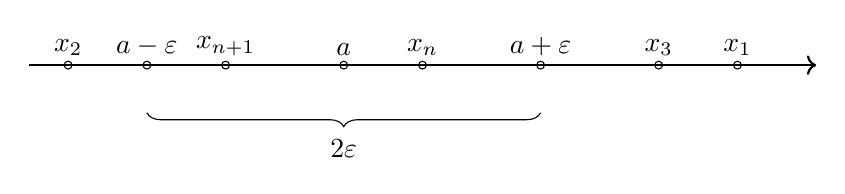
\begin{tikzpicture}
\draw[thick,->] (0,0) -- (10,0);
\draw (0.5,0) node[circle,draw,scale=0.3]{} node[above] {$x_2$};
\draw [decorate,decoration={brace,amplitude=5pt,mirror,raise=4ex}]
  (1.5,0) node[circle,draw,scale=0.3]{} node[above]{$a-\varepsilon$} -- (6.5,0) node[midway,yshift=-3em]{$2 \varepsilon$} node[circle,draw,scale=0.3]{} node[above]{$a+\varepsilon$};
%\draw [Parenthesis-Parenthesis,] (2,0) node[above] {$a-\varepsilon$} -- (7,0) node[above] {$a+\varepsilon$};
\draw (2.5,0) node[circle,draw,scale=0.3]{} node[above] {$x_{n+1}$};
\draw (4,0) node[circle,draw,scale=0.3]{} node[above] {$a$};
\draw (5,0) node[circle,draw,scale=0.3]{} node[above] {$x_n$};
%\draw (7,0) node[circle,draw,scale=0.3]{} node[above] {$a+\varepsilon$};
\draw (8,0) node[circle,draw,scale=0.3]{} node[above] {$x_3$};
\draw (9,0) node[circle,draw,scale=0.3]{} node[above] {$x_1$};
\end{tikzpicture}
\end{center}

以$a$点为中心的线段不论取的多小(其长度为$2\varepsilon$),一切$x_n$点从某点起,必全部落在这线段之内,这样在线段之外一定只有有限长度个点了,表示极限的点$a$表示为数列数值的凝聚中心.

\subsection{数列极限的基本性质}
%局部性
\begin{proposition}
\rm {\color{red} (局部性)} 若$\lim x_n = a$,又$a > p$,那么存在某个正整数$N$,当$n > N$时,一切$x_n$都满足$x_n > p$.
\end{proposition}

%保号性
\begin{proposition}
\rm {\color{red} (保号性)} 若$\lim x_n = a$,有$a > 0$,那么存在某个正整数$N$,当$n > N$时,一切$x_n$都满足$x_n > 0$.
\end{proposition}

%保值性?
\begin{proposition}
\rm {\color{red} (局部性一个推广)} 若$\lim x_n = a$,且$a \neq 0$,则必有充分远的$x_n$值,其绝对值大于某个正数$r$
$$
|x_n| > r > 0 ~ (n > N).
$$
{\color{blue} 性质1的推论}.
\end{proposition}

%有界性
\begin{proposition}
\rm {\color{red} (极限存在必有界)} 若$\lim x_n = a$,则$(x_n)$必有界.
\end{proposition}

\begin{proof}
我们知道任意给定一个$\varepsilon > 0$,可以找到正整数$N$,使得当$n > N$时的一切$x_n$都满足$ a-\varepsilon < x_n < a + \varepsilon$,因此当$n > N$是存在一个界数使得$|x_n| < M$. 接着再考虑$n \leq N$时,注意这时候只有有限个$x_n$,我们把$M$和它们放在一起,取它们里面绝对值最大的数$M'$,即有$|x_n| \leq M'$.
\end{proof} 

%极限唯一
\begin{proposition}
\rm {\color{red} (极限唯一)} 若同时有$\lim x_n = a,\; \lim x_n = b$,则$a = b$.  
\end{proposition}

\begin{proof}
假设$a \neq b$,不是一般性设$a < b$,在它们中间找一个$r$使得$a < r < b$. 由于$\lim x_n = a$,由局部性我们可以知道在从某一项起有$|x_n| < a +\varepsilon < r$; 再由于$\lim x_n = b$,有局部性我们可以知道从某一项起有$r< b- \varepsilon <|x_n|$. 综上就造成矛盾,所以$a = b$.
\end{proof}

\subsection{数列无穷小和无穷大}

\begin{definition}
\rm 若给定数列当$n \rightarrow \infty$的极限为零,则称此数列为$n \rightarrow \infty$时的{\color{red}无穷小量}. 同理若数列当$n \rightarrow \infty $的极限为无穷大,则称此数列为$n \rightarrow \infty$时的{\color{red}无穷大量}.
\end{definition}

\begin{proposition}
\rm {\color{red} (无穷小和无穷大的相互转换)} 若$(x_n)$为无穷小量且$x_n \neq 0$,那么$(\frac{1}{x_n})$为无穷大量. 反之亦然.
\end{proposition}

\begin{proposition}
\rm {\color{red} 常用无穷大},当$n \rightarrow \infty$时
\begin{enumerate}
	\item 
	$$
	\ln^\alpha n \ll n^\beta \ll a^n \ll n! \ll n^n,\; \alpha > 0,\beta > 0 ,a > 1.
	$$
\end{enumerate}
\end{proposition}

\subsection{数列极限运算}

\begin{proposition}
\rm {\color{red} (数列相同则极限相同)} 若$x_n = y_n$,则$\lim x_n = \lim y_n$.
\end{proposition}

\begin{proposition}
\rm {\color{red} (数列比较导出极限关系)} 若恒有$x_n \leq y_n$,且各自趋于有限极限,则$\lim x_n \leq \lim y_n$.
\end{proposition}

\begin{proposition}
\rm {\color{red} 夹闭准则} {\color{blue} 见经典证明}.
\end{proposition}

\begin{proposition}
\rm 任意有限个无穷小的和亦是无穷小.
\end{proposition}

\begin{proposition}
\rm 有界数列$(x_n)$与无穷小${\alpha_n}$的乘积仍是无穷小.
\end{proposition}

\begin{proposition}
\rm 若$\lim x_n = a,\; \lim y_n =b$,则$\lim(x_n\pm y_n) = a \pm b$. 考虑两个极限的尾巴
$$
\lim (x_n \pm y_n) = a+b+ \alpha + \beta.
$$
\end{proposition}

\begin{proposition}
\rm 若$\lim x_n = a,\; \lim y_n =b$,则$\lim(x_ny_n) = ab$. 考虑两个极限的尾巴
$$
\lim x_ny_n = ab + a\beta + b\alpha + \alpha\beta.
$$
\end{proposition}


\begin{proposition}
\rm 若$\lim x_n = a,\; \lim y_n =b$,且$b\neq 0$,则$\lim \frac{x_n}{y_n} = \frac{a}{b}$. 考虑两个极限的尾巴
$$
\begin{array}{ll}
\lim \frac{x_n}{y_n} - \frac{a}{b} &= \frac{a+\alpha}{b+\beta} - \frac{a}{b} \\
&= \frac{b\alpha - a\beta}{b(b+\beta)} \\
&= \frac{1}{b+\beta}(\alpha-\frac{a}{b} \beta) \\
&= \lim \frac{1}{y_n}(\alpha-\frac{a}{b}\beta).
\end{array}
$$
显然{\color{blue}有界数列乘上无穷小还是无穷小}.
\end{proposition}

\subsection{不定式}

\begin{annotation}
$$
\frac{x_n}{y_n} \sim \frac{0}{0}
$$
\end{annotation}

\begin{annotation}
$$
\frac{x_n}{y_n} \sim \frac{\infty}{\infty}
$$
\end{annotation}

\begin{annotation}
$$
x_n y_n \sim  0 \cdot \infty
$$
\end{annotation}

\begin{annotation}
$$
x_n - y_n \sim \infty - \infty
$$
\end{annotation}

\subsection{单调数列的极限}

\begin{theorem}
\rm {\color{red}(单调有界必有极限)} 给定单调增加的数列$(x_n)$,若它有上界
$$
x_n \leq M,\; n = 1,2,\cdots
$$
则它必有一有限极限,此极限为上确界. 同理单调减少的数理$(x_n)$,若它有下界
$$
x_n \geq M, \; n = 1,2,\cdots
$$
则它必有一有限极限,此极限为下确界.
\end{theorem}

\begin{proof}
根据{\color{red}确界原理},有界必有确界. 若$(x_n)$单调增且有上界,用$a =\sup\{x_n\}$表示其上确界,由确界定义有{\color{blue}(1} $x_n \leq a$; {\color{blue}(2} 对任意的$\varepsilon > 0$,都能找到$x_n > a-\varepsilon$,特别地因为这里是$f(x)$单调增,因此对任意的$n'> n$都有$x_n' > x_n$. 综上有
$$
|x_n' -a| < \varepsilon.
$$
\end{proof}

\subsection{收敛原理}

\begin{theorem}
\rm {\color{red} (柯西收敛原理)} 数列$(x_n)$有有限极限的必要且充分条件是: 对于任意的数$\varepsilon > 0$,总存在着整数$N$,使得当$n > N$和$n' > N$时有下面不等式成立
$$
|x_n - x_{n'}| < \varepsilon.
$$
\end{theorem}

\begin{proof}
{\color{red} (必要性)} 若$\lim x_n = a$,即对任意的$\frac{\varepsilon}{2}$,能找到一个整数$N$,使得$n, n' > N$时有
$$
|x_n - a| < \frac{\varepsilon}{2},\; |x_{n'} - a| < \frac{\varepsilon}{2}
$$
成立. 那么
$$
|x_n - x_{n'}| = |(x_n -a ) + (a - x_{n'})| \leq |x_n-a| + |x_{n'}-a| < \varepsilon
$$

{\color{red} (充分性)} 若满足上述定理中的条件,{\color{blue}我们要证明$\lim x_n = a$,我们得想办法把这个$a$表示出来,这里手法将会用戴德金实数划分的结论来把这个$a$弄出来}.

在全体实数域下构造一个划分. 对于任何实数$\alpha$,若$x_n$从某项其满足不等式\[x_n > \alpha,\]则取这种实数$\alpha$归入下组$A$,其余的(即不落在$A$里面的)一起实数归入上组$A'$.

首先我们来说明这样确实产生了一个实数上的划分. 由前提条件,对于任意数$\varepsilon>0$及其对应的$N$. 若$n > N$及$n' > N$,则下面不等式成立\[x_{n'} - \varepsilon < x_n < x_{n'}+\varepsilon.\]现在我们可以看到每一个数$x_{n'} - \varepsilon$都是小于$x_n$的,所以它归入下组$A$. 另一方面$x_{n'}+\varepsilon$都大于$x_n$,所以$x_{n'}+\varepsilon$放不进去$A$,那它只能归入$A'$了,所以$A$和$A'$都是非空的. 我们的划分方式对于每一个数$\alpha$和确定序列$x_n$,要么它属于$A$或者属于$A'$. 同时$A$中实数都小于$A'$的实数. 可以来验证一下,若$\alpha > \alpha', \alpha \in A , \alpha' \in A'$,则$x_n$从某一项其也都大于$\alpha$那么显然也是大于$\alpha'$,那么$\alpha'$也应该在$A$中,这样就产生矛盾了. 因此的确产生了一个实数上的划分.

根据戴德金基本定理,有实数$a$存在它是$A$和$A'$的界数,即\[\alpha \leq a \leq \alpha', \; \alpha \in A,\alpha' \in A'.\]我们注意到当$n > N$时,$x_{n'} - \varepsilon$是一个$\alpha$,而$x_{n'} +\varepsilon$是一个$\alpha'$. 所以我们有\[x_{n'} - \varepsilon \leq a \leq x_{n'} + \varepsilon.\]即$|x_{n'}-a| \leq \varepsilon$,所以$\lim x_n = a$.

{\color{blue} 若是不用实数划分的手法,也可以构造$a_n = \inf\limits_{k \geq n} x_k$和$b_n=\sup\limits_{k \geq n} x_k$,证明$\lim a_n = \lim b_n = c$,再用一下夹逼准则$a_n \leq x_n \leq b_n$.}
\end{proof}

\subsection{上下极限}

\begin{definition}
\rm 若给定数列$(x_n)$,从它里面任选一部分项
$$
x_{n_1},x_{n_2},\cdots,x_{n_k},\cdots,\; n_1 < n_2 < \cdots < n_k < \cdots,
$$
构成一个新的数列$(x_{n_k})$称为$(x_n)$的部分数列.
\end{definition}

\begin{proposition}
\rm 若数列$(x_n)$的极限存在,则其部分数列亦必有相同的极限.
\end{proposition}

\begin{proposition}
\rm 若数列$(x_n)$任一子数列都收敛,则收敛于同于极限.
\end{proposition}

\begin{proof}
反证法,构造不收敛的子数列.
\end{proof}

\begin{theorem}
\rm {\color{red} B.Bolzano-C.Weierstrass定理} 任何有界的数列内总是可以选出可收敛的部分极限.
\end{theorem}

\begin{proof}
区间套.
\end{proof}

%https://en.wikipedia.org/wiki/Limit_inferior_and_limit_superior
\begin{definition}
\rm 序列$(x_n)$的部分极限的最大值和最小值,称为$x_n$的上极限和下极限,各记为
$$
\overline{\lim} x_n~\text{及}~\underline{\lim} x_n.
$$
\end{definition}

\subsection{常用极限}

\begin{proposition}
\rm {\color{red} 常用初等极限}
\begin{enumerate}
	\item 
	$$
		\lim\limits_{n \rightarrow \infty} \sqrt[n]{n} = 1. ~{\color{blue}\text{(取对数证明)}}
	$$
	\item
	$$
		\lim\limits_{n \rightarrow \infty} \sqrt[n]{a} = 1,\; a > 0. ~\text{(取对数证明或者伯努利不等式)}
	$$
\end{enumerate}
\end{proposition}

\subsection{不要求掌握但是极为有用的一些定理}

\begin{theorem}
\rm {\color{red} (O.Stolz定理用于判定$\frac{\infty}{\infty}$有奇效)} 若$\lim y_n = +\infty$,且至少从某一项开始在$n$增大时$y_n$亦增大,即$y_{n+1} > y_n$,则
$$
\lim\frac{x_n}{y_n} = \lim \frac{x_n - x_{n-1}}{y_n - y_{n-1}}.
$$
等式右边极限(有限或者无穷)存在推出左边有相同的极限. {\color{blue} 我们可以先用这个定理把极限确定下,在尝试转换思路求$\lim\limits_{n \rightarrow \infty} (\frac{x_n}{y_n} - A) = 0$,也许会有奇效}.
\end{theorem}

\newpage
\section{函数极限}

\subsection{函数极限的定义}

\begin{definition}
\rm 设定义在区间$\mathcal{X}$上的函数$f(x)$,点$x_0$是其一个聚点,若给定任意的$\varepsilon  > 0$,都能找到$\delta > 0$,使得满足$|x-x_0| < \delta$,都有
$$
|x-A| < \varepsilon,
$$
则称函数$f(x)$在$x_0$处的存在有限极限为$A$.
\end{definition}

\subsection{函数左右极限}
\begin{definition}
\rm 设定义在区间$\mathcal{X}$上的函数$f(x)$,点$x_0$是其一个聚点. 若给定任意的$\varepsilon > 0$,都能找到$\delta > 0$,使得对$x \in (x_0-\delta,x_0)$满足
$$
|f(x_0)-A| < \varepsilon.
$$
则称$f(x)$在$x_0$处有{\color{red}左极限}存在. 同理若使得$x \in (x_0,x_0 +\delta)$也满足上述不等式,则称$f(x)$在$x_0$处有{\color{red}右极限}.
\end{definition}

\begin{proposition}
\rm {\color{red} (极限存在的充要条件) }函数$f(x)$在点$x_0$处极限存在的充分必要条件是在$x_0$处的左极限和右极限都存在且相同.
\end{proposition}

\subsection{用数列的语言来描述函数极限}

\begin{annotation}
\rm  将数列可以视为函数$f : n \to a_n$,即自变量为自然数的函数. 则当$n \to \infty$时$f(n)$的极限,就可以直接用函数极限定义来表示.  
\end{annotation}

\begin{definition}
\rm 数列极限是函数极限的特殊情形. 
\end{definition}

\begin{theorem}\label{func-limit: Heine}
\rm 设定义在区间$\mathcal{X}$上的函数$f(x)$,点$x_0$是其一个聚点. $f(x)$在$x_0$处存在有限极限$A$当且仅当任意选自$\mathcal{X}$上以$x_0$为极限的数列$(x_n)$,其对应函数值的数列$(f(x_n))$极限均存在且等于$A$. {\color{red} 这是一个非常重要的定理,使得我们可以用数列的语言来描述函数极限,因此通常我们选取特殊的数列来描述函数的极限!}
\end{theorem}

\begin{proof}
\rm 首先是如何构造一组趋于$x_0$的极限$(x_n)$. 在给定一趋于零的数列${\delta_n}$之后,由$x_0$是$\mathcal{X}$的聚点,那么恒能选出$x = x_n$使得$|x_n - x_0| < \delta_n$,因此$\lim x_n = x_0$. 

\emph{必要性}\ 若$f(x)$在$x_0$存在有限极限$A$. 则对任意的$\varepsilon > 0$,存在$\delta > 0$,使得当$|x-x_0| < \delta$时满足$|f(x)-A| < \varepsilon$. 在充分大$n$时,亦有$|x_n - x_0| < \delta$,因此也有$|f(x_n)-A| < \varepsilon$,即数列$(f(x_n))$的极限也等于$A$. 

\emph{充分性}\ 若任意选自$\mathcal{X}$上以$x_0$为极限的数列$(x_n)$,其对应函数值的数列$\{f(x_n)\}$极限均存在且等于$A$. 若假设$A$不是$f(x)$在$x_0$处的极限,那么存在$\varepsilon > 0$,使得对任意的$\delta > 0$满足当$|x-x_0| < \delta$时,都有$|f(x)-A| \geq \varepsilon$. 因此取一趋于零的$(\delta_n)$,对任意一$\delta = \delta_n$,我们都可以挑一个$x_n$使得$|x_n' -x_0| < \delta_n$,这样我们就得到的${x_n'}$同样是以$x_0$为极限,但是此刻数列$(f(x_n))$的极限并不等于$A$,因此与前提矛盾. 即$A$是$f(x)$在$x_0$处的极限.  
\end{proof}



\subsection{两个重要极限}

\begin{proposition}
$$
\lim\limits_{x \rightarrow 0} \frac{\sin x}{x} = 1.
$$
\end{proposition}

\begin{proof}
几何证明的手法,或者直接上洛必达.
\end{proof}

\begin{proposition}
\rm {\color{blue}$\lim\limits_{x \rightarrow 0} \frac{\sin x}{x}$延伸的极限}
\begin{enumerate}
	\item $\frac{0}{0}$
	$$
	\lim\limits_{x \rightarrow 0} \frac{\tan x}{x} = \lim\limits_{x \rightarrow 0} \frac{\frac{\sin x}{\cos x}}{x} = 1
	$$
	\item $\frac{0}{0}$
	$$
	\lim\limits_{x \rightarrow 0} \frac{1-\cos x}{x^2} = \lim\limits_{x \rightarrow 0} \frac{2\sin^2\frac{x}{2}}{4(\frac{x}{2})^2} = \frac{1}{2}
	$$
	\item $\frac{0}{0}$
	$$
	\lim\limits_{x \rightarrow 0} \frac{\tan x-\sin x}{x^3} = \lim\limits_{x \rightarrow 0} \frac{1-\cos x}{x^2\cos x}\frac{\sin x}{x} = \frac{1}{2}
	$$
	\item $\infty - \infty$ 通过和差化积是有点麻烦的,但是可以算的,这里用一点小trick,调整一下自变量使得$\alpha = \frac{\pi}{2} - x$
	$$
		\lim\limits_{x \rightarrow \frac{\pi}{2}} \sec x -\tan x = \lim\limits_{\alpha \rightarrow 0} \csc x - \cot x = \lim\limits_{\alpha \rightarrow 0} \frac{1-\cos x}{\sin x} = \lim\limits_{\alpha \rightarrow 0} \frac{1-\cos x}{x^2} \frac{x}{\sin x} x = 0.
	$$
\end{enumerate}
\end{proposition}

\begin{proposition}
$$
\lim\limits_{x \rightarrow +\infty} (1+\frac{1}{x})^x = e.
$$
\end{proposition}

\begin{proof}
单调有界.
\end{proof}

\begin{proposition}
\rm $\lim\limits_{x \rightarrow +\infty} (1+\frac{1}{x})^x = e$延伸出来的极限
\begin{enumerate}
	\item $\frac{0}{0}$
	$$
	\lim\limits_{x \rightarrow 0} \frac{\log_a(1+x)}{x} = \log_a e.
	$$
	\hints\ 直接用对数函数的性质,把分母$x$放到对数函数里面就行,对数函数里面的极限是$e$.当$a=e$时极限的结果就是很漂亮的$1$.
	\item $\frac{0}{0}$
	$$
	\lim\limits_{x \rightarrow 0} \frac{a^x - 1}{x} = \ln a
	$$
	\hints\ 遇到这样略微有些复杂的表达式,直接考虑换元. 让$\beta = a^x -1$,则$\beta \rightarrow 0$. 原式就变成了$\lim\limits_{\beta \rightarrow 0} \frac{\beta}{\log_a(\beta+1)}$. 变成了上面我们熟悉样子.	
	\item $\frac{0}{0}$ 
	$$
	\lim\limits_{x \rightarrow 0} \frac{(1+x)^\mu-1}{x} = \mu
	$$
	\hints\ 还是考虑换元,但是不要换的太彻底,适可而止即可. $\beta = (1+x)^\mu - 1$,其中$\beta \rightarrow 0$. 我们可以得到一个有趣的等式$\mu \ln(1+x) = \ln(1+\beta)$. 到这里就够了,不用把$\beta$把$\alpha$表示出来. 我们把原式现在整理如下\[\frac{(1+x)^\mu-1}{x} = \frac{\beta}{x} = \frac{\beta}{\ln(1+\beta)}\cdot\frac{\ln(1+x)}{x}\cdot \mu,\]又变成了我们熟悉的样子,两边的极限都是$1$,所以最后的整体的极限为$\mu$.	
	\item $1 \cdot \infty$ 若$\lim\alpha(x) = 0,\lim\beta(x) = \infty$,且$\lim\alpha(x)\beta(x) = A$
	$$
	\lim(1+\alpha(x))^{\beta(x)} = e^A.
	$$
	\hints\
	$$
	(1+\alpha(x))^{\beta(x)}  =e^{\beta(x)\ln(1+\alpha(x))} = e^{\alpha(x)\beta(x)}.
	$$
	\item $\frac{0}{0}$ 若$\lim \alpha(x) = 0$,且$\lim\beta(x)\alpha(x) = 0$
	$$
	\lim\frac{(1+\alpha(x))^{\beta(x)}-1}{\alpha(x)\beta(x)} = 1.
	$$
	\hints\ 
	$$
	(1+\alpha(x))^{\beta(x)}-1 = e^{\beta(x)\ln(1+\alpha(x))} - 1
	$$
\end{enumerate}
\end{proposition}

\subsection{常用极限}

\begin{proposition}
\rm {\color{red}常用极限,需熟记}
\begin{enumerate}
	\item 
	$$
	\lim\limits_{x \rightarrow 0} \sqrt[m]{1+x} = 1.
	$$
	\hints\ 函数的连续性.
\end{enumerate}
\end{proposition}

\subsection{函数极限的基本性质}

%局部性
%保号性
%有界性
\begin{proposition}
\rm 若$\lim\limits_{x \rightarrow a} f(x) = A$,则对于充分接近$a$的$x$的函数值是有界的
$$
|f(x)-A| \leq M ,\; |x-a| < \delta.
$$
即在$x_0$某个去心邻域有界. {\color{blue} 注意这里和序列极限$\lim x_n = b$,而导致整个$(x_n)$有界是区别的,因为这里当$x-a < -\delta$或者$x-a > \delta$可能有无限多个函数值的,它们是否有界是无法确定的}. {\color{red} 命题反过来不一定正确,即有界不一定收敛}.
\end{proposition}

\subsection{函数极限运算}

\begin{proposition}
\rm 若$\lim\limits_{x \rightarrow a} f(x) = A$和$\lim\limits_{x \rightarrow a} g(x) = B$,则函数
$$
\begin{array}{ll}
\lim\limits_{x \rightarrow a} (f(x) \pm  g(x)) &= A \pm B,\\
\lim\limits_{x \rightarrow a} f(x) \cdot g(x) & = A\cdot B, \\
\lim\limits_{x \rightarrow a} \frac{f(x)}{g(x)} &= \frac{A}{B}.
\end{array}
$$
\end{proposition}

\subsection{不定式}

\begin{annotation}
$$
\frac{0}{0},\; \frac{\infty}{\infty},\; 0\cdot \infty,\; \infty-\infty.
$$
\end{annotation}

\begin{proposition}
\rm {\color{red}常见$\frac{\infty}{\infty}$极限}.
\begin{enumerate}
	\item
	$$
		\lim \frac{a_nx^{n} + a_{n-1}x^{n-1} + \cdots + a_1x + a_0}{b_mx^{m} + b_{m-1}x^{m-1} + \cdots + b_1x + b_0} = \left\{ \begin{array}{ll}
		\frac{a_n}{b_m} & n=m \\
		\infty & n > m \\
		0 & n < m 
\end{array} \right.
	$$
\end{enumerate}
\end{proposition}

\begin{proposition}
\rm {\color{red}常见$\frac{0}{0}$极限}
\begin{enumerate}
	\item 
	$$
	\lim\limits_{x \rightarrow 0} \frac{\sqrt[m]{1+x}-1}{x} = \frac{1}{m}.
	$$
\end{enumerate}
\end{proposition}

\subsection{单调函数的极限}

\begin{theorem}
\rm \redt{单调有界则收敛} 若单调增大函数$f(x)$在区域$\mathcal{X}$内变动着. 区域$\mathcal{X}$以大于一切$x$值的数$a$(它可以是有限的数,或者等于$+\infty$)作为聚点,若在这时函数$f(x)$在$\mathcal{X}$上有上界
$$
\forall x \in \mathcal{X},\;f(x) \leq M.
$$
则当$x \rightarrow a$时$f(x)$有一有限极限. 
\end{theorem}

\begin{proof}
若$f(x)$上有界,考虑$f$在$\mathcal{X}$上变动构成的集合$\{f(x)\}$,即$\{f(x)\}$是有上界的,那么根据确界原理,$\{f(x)\}$有上确界,设其为$A$,接下来我们证明$A$就是$f(x)$趋向于$a$的极限.

给定任意$\varepsilon > 0$,根据上确界的性质,可以找到一个$x' < a$,使得$f(x') > A-\varepsilon$. 再由于$f(x)$是单调增的,所以当$x > x'$时,都有$f(x) > A -\varepsilon$,其上界也很容易得到$f(x) \leq A < A+\varepsilon$,所以综上当$x > x'$有
$$
A-\varepsilon < f(x) < A+\varepsilon.
$$
这里$\delta$的取值取决于$a$的取值,若$a$是一个有限的数,那么$\delta = a-x'$即可,若$a = +\infty$,则取$\Delta = x'$. 
\end{proof}

\begin{corollary}
\rm \redt{数列的语言应用} 若单调增大函数$f(x)$在区域$\mathcal{X}$内变动着. 区域$\mathcal{X}$以大于一切$x$值的数$a$(它可以是有限的数,或者等于$+\infty$)作为聚点,且在这时函数$f(x)$在$\mathcal{X}$上有上界. 那么任意以取自$\mathcal{X}$上以$a$的单调增大数列$(x_n)$,它的极限等于$f(x)$在$a$点处的极限. 
\end{corollary}


\subsection{函数收敛的判定方法}

\begin{theorem}
\rm \redt{柯西判别} 函数$f(x)$当$x$趋于$a$时有一有限极限的充分必要条件为,对于任意$\varepsilon > 0$必存在着$\delta > 0$,只需要满足
$$
|x-a| < \delta,\; |x'-a| < \delta.
$$
就能使得下面不等式成立
$$
|f(x)-f(x')| < \varepsilon.
$$
\end{theorem}

\begin{proof}
{\color{blue}充分性显然,必要性可以通过用数列描述函数极限的方法,配合数列中有限极限存在的充要来条件来进行证明}.
\end{proof}

\subsection{无穷小及无穷大的分阶}


\begin{definition}
\rm 给定两个无穷小$\alpha$和$\beta$
\begin{enumerate}
	\item 若$\frac{\beta}{\alpha}$有一异于零的有限极限,则称$\alpha$和$\beta$是{\color{red}同阶无穷小};
	\item 若$\frac{\beta}{\alpha}$趋于无穷小,则称$\beta$是$\alpha$的{\color{red} 高阶无穷小},记做$\beta = o(\alpha)$.
	同时$\alpha$是$\beta$的低阶无穷小;
\end{enumerate}
\end{definition}

\begin{definition}
\rm 为了更精确地比较无穷小的性态,需要用数字来表示它们的阶,在这种情形下,我们首先在所研究的无穷小内选出一个作为一种"标准",把它称为{\color{red}基本无穷小}.
\end{definition}

\begin{definition}
\rm 若$\beta$与$\alpha^k$是同阶的无穷小量,选定$\alpha$为基本无穷小,则称$\beta$是基本无穷小$\alpha$的$k$阶无穷小.
\end{definition}

\begin{definition}
\rm 给定两个无穷小$\alpha$和$\beta$,若它们的差$\gamma = \beta - \alpha$是比$\alpha$和$\beta$中任何一个更高阶的无穷小,则称$\alpha$和$\beta$为{\color{red}等价无穷小},记做$\alpha \sim \beta$.
\end{definition}

\begin{proposition}
\rm {\color{red} (等价无穷小的充要条件)} 给定两个无穷小$\alpha$和$\beta$,若它们是等价无穷小当且仅当$\lim \frac{\beta}{\alpha} = 1$.
\end{proposition}

\begin{proof}
经常看见的定义实际是一个充要条件,首先证明{\color{blue}充分性},设$\delta = \frac{\beta}{\alpha} - 1$,所以有$\lim \delta = 0$. 那么其差为
$$
\gamma = \delta \alpha,
$$
很容易得到$\lim \frac{\gamma}{\alpha} =\lim \delta = 0$和$\lim \frac{\gamma}{\beta} = \lim \delta\cdot\frac{\alpha}{\beta} = 0$,即$\gamma$是比$\alpha$和$\beta$更高阶的无穷小.

{\color{blue}必要性} 若$\alpha$和$\beta$是等价无穷小,那么
$$
\lim \frac{\beta-\alpha}{\alpha} = \lim (\frac{\beta}{\alpha} - 1) = 0,
$$
所以$\lim \frac{\beta}{\alpha} = 1$.
\end{proof}


\begin{definition}
\rm 若选定$\alpha$为基本无穷小,则形如$c\cdot \alpha^k$就被称为{\color{red}最简单的无穷小},其中$c$是一个常数,而$k > 0$. 设$\beta$是关于$\alpha$的$k$阶无穷小,即
$$
\lim \frac{\beta}{\alpha^k} = c,
$$
其中$c$是异于零的有限数,则
$$
\lim \frac{\beta}{c\alpha^k} = 1,
$$
因此$\beta$和$c\alpha^k$为等价无穷小. 与给定无穷小$\beta$等价的最简单的无穷小$c\alpha^k$被称为$\beta$的{\color{red}主部}.
\end{definition}

\begin{annotation}
\rm 设$\beta \sim c\alpha^k$,即$\beta = c\alpha^k + \gamma$,其中$\gamma = o(c\alpha^k)$. 可以想象,再从$\gamma$也可以分出主部$\gamma = c'\alpha^{k'} + \delta$,其中$k' > k$,而$\delta = o(c'\alpha^{k'})$,余类推. {\color{blue}是不是感觉你可以把泰勒展开式由此推出来? 但是这种方法太低效了,但是它却能帮你更好的理解等价无穷小的概念}.
\end{annotation}

\begin{proposition}
\rm {\color{red} (等价无穷小的替换) }给定4个$x \rightarrow x_0$时的无穷小量$\alpha_1,\alpha_2,\beta_1,\beta_2$,且$\alpha_1 \sim \beta_1, \alpha_2 \sim \beta_2$. 若极限$\lim\limits_{x \rightarrow x_0} \frac{\alpha_1}{\alpha_2}$存在(有限或者无穷大),则
$$
\lim\limits_{x \rightarrow x_0} \frac{\alpha_1}{\alpha_2} = \lim\limits_{x \rightarrow x_0} \frac{\beta_1}{\beta_2}.
$$
乘法同理. 若极限$\lim\limits_{x \rightarrow x_0} \frac{\beta_1}{\beta_2} = A, \; A \neq -1$,则
$$
\alpha_1 + \alpha_2 \sim \beta_1 + \beta_2.
$$ 
除法同理.
\end{proposition}

\begin{proof}
除法证明
$$
\lim\limits_{x \rightarrow x_0} \frac{\alpha_1}{\alpha_2}= \lim\limits_{x \rightarrow x_0} \frac{\alpha_1}{\beta_1} \cdot \frac{\beta_1}{\beta_2} \cdot \frac{\beta_2}{\alpha_2} = \frac{\beta_1}{\beta_2}. 
$$
加法证明,设$\gamma_1 = \frac{\alpha_1}{\beta_1} - 1,\gamma_2 = \frac{\alpha_2}{\beta_2} - 1$,则
$$
\lim\limits_{x \rightarrow x_0} \frac{\alpha_1+\alpha_2}{\beta_1 + \beta_2} = \lim\limits_{x \rightarrow x_0} \frac{\beta_1(1+\gamma_1) + \beta_2(1+\gamma_2)}{\beta_1 + \beta_2} = \lim\limits_{x \rightarrow x_0} \left( \frac{1+\gamma_1}{1+\frac{\beta_2}{\beta_1}} + \frac{1+\gamma_2}{1+\frac{\beta_1}{\beta_2}} \right) = 1. 
$$
\end{proof}

\begin{proposition}
\rm  {\color{red} 常用无穷大的比较}
\begin{enumerate}
	\item 当$x \rightarrow +\infty$时
	$$
		\ln^\alpha x \ll x^\beta \ll a^x, \;\alpha > 0 ,\beta > 0,a > 1 
	$$
\end{enumerate}
\end{proposition}

\begin{proposition}
\rm 当$x \to 0$时的常用等价无穷小
$$
\begin{array}{ll}
x \sim \sin x \sim \tan x \sim \arcsin x \sim \arctan x \sim e^x-1 \sim \ln(1+x) \\
\end{array}
$$
\end{proposition}

\subsection{洛必达法则}

\begin{definition}
\rm 若real-value函数$f$和$g$都在去心邻域$\tilde{U}(c,\delta)$可导,有
$$
\lim\limits_{x \rightarrow c} f(x) = \lim\limits_{x \rightarrow c} g(x) = 0 ~\text{或者}~ \lim\limits_{x \rightarrow c} g(x) = \infty,
$$
且对任意$x \in \tilde{U}$都有$g'(x) \neq 0$,同时有$\lim\limits_{x \rightarrow c}\frac{f'(x)}{g'(x)}$存在,那么
$$
\lim\limits_{x \rightarrow c} \frac{f(x)}{g(x)} = \lim\limits_{x \rightarrow c} \frac{f'(x)}{g'(x)}.
$$
\end{definition}

\begin{proof}
首先来看一个比较特殊的情况,除满足上述条件之外,若还满足$f(c) = g(c) = 0$,并且$g'(c) \neq 0$,那么
$$
\lim\limits_{x \rightarrow c}  \frac{f(x)}{g(x)} = \lim\limits_{x \rightarrow c} \frac{f(x) - f(c)}{g(x) - g(c)} = \lim\limits_{x \rightarrow c} \frac{ \frac{f(x) - f(c)}{x-c}}{\frac{g(x) - g(c)}{x-c}} = \frac{f'(c)}{g'(c)} = \lim\limits_{x \rightarrow c} \frac{f'(x)}{g'(x)}.
$$
下面来严格证明分两种情况来证明,由于$\tilde{U}$在$c$这里间断,后面需要频繁使用到柯西中值定理,所以自然地在$\title{U}$的两端来分析,取开区间$\mathcal{I}$以$c$点为端点,且$\mathcal{I} \subset \tilde{U}$. {\color{blue}注意到条件满足对任意的$x \in \mathcal{I}$有$g'(x) \neq 0$,并且$g$在$\mathcal{I}$上是连续的,那么是可以在$\mathcal{I}$里面找到一个足够小的区间使得$g(x)\neq 0$,那这个小区间代替$\mathcal{I}$}. 

我们定义$m(x) = \inf\frac{f'(\alpha)}{g'(\alpha)}$和$M(x) = \sup\frac{f'(\alpha)}{g'(\alpha)}$其中$x \in \mathcal{I}$,$\alpha$取遍$x$和$c$之间的数({\color{blue} 为什么确保可以取到确界? 任意$\alpha$处$f$和$g$导数均有意义}). 在确定$x$之后,我们再取定$x$和$c$之间一点$y$,结合柯西中值定理可以保证在它们之间找到一个$c$使得
$$
 m(x) \leq \frac{f(x) - f(y)}{g(x) - g(y)} = \frac{f'(\alpha)}{g'(\alpha)} \leq M(x).
$$
注意为什么这里可以保证$g(x) - g(y) \neq 0$? 假设存在$g(x) = g(y)$, 那么根据罗尔定理,就存在一点$p$使得$g'(p) = 0$,这是和前提条件$\forall x \in \bar{U},\;g'(x) \neq 0$矛盾的.

{\color{blue}情况一}:$\lim\limits_{x \rightarrow c} f(x) = \lim\limits_{x \rightarrow c} g(x) = 0.$

对任意的$x \in \mathcal{I}$, 取$y$位于$x$和$c$之间,为了得到$\frac{f(x)}{g(x)}$,我们让
$$
m(x) \leq \frac{f(x) - f(y)}{g(x) - g(y)} = \frac{\frac{f(x)}{g(x)} - \frac{f(y)}{g(x)}}{1 - \frac{g(y)}{g(x)}} \leq M(x).
$$
当$y \rightarrow c$时,$\frac{f(y)}{g(x)}$和$\frac{g(y)}{g(x)}$都趋向于$0$,所以
$$
m(x) \leq \frac{f(x)}{g(x)} \leq M(x).
$$

{\color{blue}情况二}:$\lim\limits_{x \rightarrow c} g(x) = \infty.$

对任意的$x \in \mathcal{I}$, 取$y$位于$x$和$c$之间. 如果我们还是用上面的分式,直接尝试把$\frac{f(x)}{g(x)}$构造出来,尝试分式对$y \rightarrow c$取极限的时候,显然是无法处理的. {\color{blue}同时你注意到在当前条件下是对$\lim\limits_{x \rightarrow c} f(x)$是没有特别说明的,言下之意它不会对我们的证明产生影响}. 现在我们考虑把前面分式上下都除以$g(y)$,同时上下取负,即
$$
m(x) \leq \frac{f(y) - f(x)}{g(y) - g(x)} = \frac{\frac{f(y)}{g(y)} - \frac{f(x)}{g(y)}}{1 - \frac{g(x)}{g(y)}} \leq M(x).
$$
那么当$y \rightarrow c$时,$\frac{f(x)}{g(y)}$和$\frac{g(x)}{g(y)}$都是趋于$0$,那么此刻关键是我们如何需要考虑$\lim\limits_{y \rightarrow c}\frac{f(y)}{g(y)}$? 让$S_x = \SET{y}{y~\text{位于}~x~\text{和}~c~\text{之间}}$, 我们取遍$y \in S_x$, 我们可以得到得到一个有界数列$\{\frac{f(y)}{g(y)}\}$({\color{red} 为什么有界? $f$和$g$在$[x,c]$上连续}),我们考虑其上下极限
$$
m(x) \leq \lim\limits_{y \rightarrow c }\inf\frac{f(y)}{g(y)} \leq \lim\limits_{y \rightarrow c }\sup\frac{f(y)}{g(y)} \leq M(x).
$$

当对$m(x)$和$M(x)$也取极限$x \rightarrow c$时,有
$$
\lim\limits_{x \rightarrow c} m(x) = \lim\limits_{x \rightarrow c} M(x) = \lim\limits_{x \rightarrow c} \frac{f'(x)}{g'(x)}.
$$
对{\color{blue}情况一}使用{\color{red} 夹逼准则},可以很快得到$\lim\limits_{x \rightarrow c} \frac{f(x)}{g(x)} = \lim\limits_{x \rightarrow c} \frac{f'(x)}{g'(x)}$. 对{\color{blue} 情况二 }也同样使用{\color{red} 夹逼准则},可以得到
$$
\lim\limits_{y \rightarrow c }\inf\frac{f(y)}{g(y)} = \lim\limits_{y \rightarrow c }\sup\frac{f(y)}{g(y)} = \lim\limits_{x \rightarrow c} \frac{f'(x)}{g'(x)},
$$
上下极限相等可以马上得到$\lim\limits_{x \rightarrow c} \frac{f(x)}{g(x)} = \lim\limits_{x \rightarrow c} \frac{f'(x)}{g'(x)}$. 最终证毕.
\end{proof}

\newpage
\section{函数连续及其间断}

\subsection{函数连续的定义}

\begin{annotation}
\rm {\color{red} (motivation)} 在研究$x$趋向于$x_0$的极限时候,即$\lim\limits_{x \rightarrow x_0} f(x)$,并不要求$x$可以取到$x_0$,即使$f(x_0)$有定义,极限也不依赖它. 自然地,现在我们特别地考虑若$f(x_0)$有定义,且$\lim\limits_{x \rightarrow x_0}f(x) = f(x_0)$,这种情形下我们就说$f$在$x_0$处{\color{red}连续},其他情况下则说$f$在$x_0$这里有{\color{red}间断}. {\color{blue} 函数连续是一个局部的性质}.
\end{annotation}


\subsection{函数连续性在计算极限时的应用}

\begin{proposition}
\rm {\color{red} (推进极限符号)} 若函数$f(x)$在$\mathbb{R}$上连续,则
$$
\lim\limits_{x \rightarrow x_0} f(g(x)) = f(\lim\limits_{x \rightarrow x_0}g(x)),
$$
只需要极限$\lim\limits_{x \rightarrow x_0}g(x)$存在.
\end{proposition}

\begin{proof}
\rm 若$\lim\limits_{x \rightarrow x_0}g(x) = t$,由\ref{func-limit: Heine},可知
$$
\lim\limits_{x \rightarrow x_0}g(x) = \lim\limits_{n \to \infty} g(a_n) = t,
$$
其中$\lim\limits_{n \to \infty}a_n = x_0$. $f(x)$在$t$连续,于是
$$
\lim\limits_{x \rightarrow t} f(x) = \lim\limits_{n \to \infty} f(g(a_n)) = f(\lim\limits_{n \to \infty}g(a_n)) = f(\lim\limits_{x \rightarrow x_0}g(x)).
$$
由于$(a_n)$是任意,那么实际上式就保证了$\lim\limits_{x \rightarrow x_0}(f \circ g) (x)$极限存在,且$\lim\limits_{n \to \infty} f(g(a_n)) = \lim\limits_{x \rightarrow x_0}f(g(x))$. 综上证闭.	
\end{proof}

\begin{annotation}
\rm 从函数连续的定义上可知$\lim\limits_{x \rightarrow x_0}f(x) = f(x_0)$,即在某点连续,这点的极限就是其函数值,这个关系对求极限是非常有用. 例如
$$
\lim\limits_{x \rightarrow 1} \sqrt[m]{x} = 1.
$$
其中$\sqrt[m]{x}$是连续的.
\end{annotation}

%严格定义

\subsection{连续函数的算术运算}

\begin{theorem}
\rm 若函数$f(x)$和$g(x)$都在区间$\mathcal{X}$上变动着,且都在点$x_0$处连续,则函数
$$
f(x) \pm g(x),\; f(x)\cdot g(x), \; \frac{f(x)}{g(x)}~(g(x_0) \neq 0)
$$
也在都$x_0$处连续.
\end{theorem}

\begin{proof}
{\color{blue}与相关函数的极限联系起来即可}.
\end{proof}

\subsection{单侧连续和间断分类}

\begin{definition}
\rm {\color{red} (单侧极限) }若$f(x)$在$x_0$处是左(右)连续,只需要满足下面关系式
$$
\begin{array}{ll}
f(x_0^-) = \lim\limits_{x \rightarrow x_0^-} = f(x_0). \\
\left[ f(x_0^+) = \lim\limits_{x \rightarrow x_0^+} = f(x_0) \right]
\end{array}
$$
{\color{blue}用自然语言说就是求极限过程中,我们既可以从左边接近$x_0$,也可以从右边接近$x_0$,于是就有了单侧极限的概念}.
\end{definition}

\begin{theorem}
\rm {\color{red} (连续的充要条件)} 函数$f(x_0)$在点$x_0$处连续当且仅当其左极限和右极限都存在且相等.
\end{theorem}

\begin{definition}
\rm 函数$f(x)$可能在$x_0$处存在两类间断点
\begin{enumerate}
	\item $x_0$处单侧极限存在但是不等于$f(x_0)$,则$f(x)$在$x_0$处有间断点,称其为{\color{red}普通间断点}或者{\color{red}第一类间断点}. 若左右极限存在且相等,则称其为\redt{可去间断点}; 若左右极限存在且不相等,通常说在$f(x)$在$x_0$处有{\color{red}跃度}. 
	\item $x_0$处单侧极限是无穷或者根本不存在,则$f(x)$在$x_0$处有间断点,称其为{\color{red} 第二类间断点}.
\end{enumerate}
\end{definition}

\subsection{单调函数的连续性和间断}

\begin{theorem}
\rm {\color{red} (单调函数上的间断点)} 若单调函数$f(x)$在区间$\mathcal{X}$内有间断点,那么只能是第一类间断点.
\end{theorem}

\begin{proof}
若$f(x)$是单调增的,且在$x_0$处有间断点,那么考虑其左极限,当$x < x_0$时,都有$f(x) < f(x_0)$,即$f(x)$在趋近于$x_0$过程中是有界,那么根据单调函数有界则必有有限极限的定理,则有
$$
\lim\limits_{x \rightarrow x^-} f(x) \leq f(x_0).
$$
若可以取到等号,则$f(x)$在$x_0$处左连续,反之$f(x)$在$x_0$处有跃度,所以是第一类间断点. 同理也可以考虑右极限.
\end{proof}

\begin{theorem}
\rm {\color{red} (单调函数连续性判别)} 若在区间$\mathcal{X}$上的单调函数$f(x)$的函数值都含于区间$\mathcal{Y}$,且把整个$\mathcal{Y}$都填满了,即$\forall y \in \mathcal{Y}$,都存在一个$x \in \mathcal{X}$使得$f(x) = y$,则$f(x)$在$\mathcal{X}$上连续.
\end{theorem}

\begin{proof}
若$f(x)$为单调增的,假设$f(x)$在$\mathcal{X}$在$x_0$处有间断点,即$\lim\limits_{x \rightarrow x_0 ^-} f(x) < f(x_0)$,那么$f(x_0^-)$和$f(x_0)$之间的值,$f(x)$是无法取到的,这和命题是矛盾的,所以$f(x)$在$\mathcal{X}$上连续.
\end{proof}

\subsection{初等函数的连续性}

\subsection{连续函数的复合}

\begin{theorem}
\rm 若函数$\varphi(y)$定义在区间$\mathcal{Y}$上,而函数$f(x)$定义于区间$\mathcal{X}$上,且其对应的函数值含于$\mathcal{Y}$. 若$f(x)$在$\mathcal{X}$中的一点$x_0$连续,又$\varphi(y)$在$y_0 = f(x_0)$这一点也是连续的,则复合函数$\varphi(f(x))$在点$x_0$处亦是连续的.
\end{theorem}

\subsection{一致性连续}

\begin{annotation}
\rm 在函数连续的定义中,$\delta$的选择可能不仅仅依赖$\varepsilon$,可能同样依赖于$x_0$的选择,因为函数在每个某个点上变动情况可能不一样,变动的越剧烈,$\delta$的选择可能更小,那么是否存在一种连续性$\delta$的选择只依赖$\varepsilon$呢?一致连续就运营而生了.
\end{annotation}

\begin{definition}
\rm 若对于任一数$\varepsilon > 0$,都能求出$\delta > 0$使得当满足
$$
|x-x_0| < \delta
$$
时,都有$|f(x)-f(x_0)| < \varepsilon$,不论$x_0$及$x$在定义域区间$\mathcal{X}$怎样选择,我们就称$f(x)$在$\mathcal{X}$上{\color{red}一致连续},即$\delta$是适用于一切的$x_0$.
\end{definition}

\begin{annotation}
\rm 一致性也可以表示为在$\mathcal{X}$上任意两个$x$取值,只要它们足够的近,它们对应的函数值也是相对来说足够的近. 
\end{annotation}

\begin{theorem}
\rm {\color{red} (康托定理) }若函数$f(x)$是在闭区间$[a,b]$内定义着而且连续,则它在这区间上也是一致连续的.
\end{theorem}

\begin{corollary}
\rm 若函数$f(x)$在闭区间$[a,b]$上定义着且连续. 则对任意的$\varepsilon > 0$,能求出$\delta > 0$,使得把$[a,b]$分成若干个长度小于$\delta$小区间,那么在每个小区间上$f(x)$的振幅(最大值和最小值的差)将小于$\varepsilon$.
\end{corollary}

\newpage
\section{函数导数}

\subsection{导数定义}

\begin{definition}
\rm 设函数$y=f(x)$在点$x_0$的某个邻域内有定义,当自变量$x$在$x_0$处取得增量$\Delta x$时,相应地,因变量取得增量$\Delta y = f(x_0 + \Delta x) - f(x_0)$. 如果$\frac{\Delta y}{\Delta x}$当$\Delta x$趋近于$0$时极限存在,那么称函数$y = f(x)$在$x_0$处可导,并称这个极限为函数$y=f(x)$在点$x_0$处的导数,记做$f'(x_0)$,即
$$
f'(x_0) = \lim\limits_{\Delta x \rightarrow 0} \frac{\Delta y}{\Delta x} = \lim\limits_{\Delta x \rightarrow 0} \frac{f(x_0 + \Delta x) - f(x_0)}{\Delta x}.
$$
\end{definition}

\begin{definition}
\rm {\color{red} 导数的记法}
\begin{enumerate}
	\item $\frac{dy}{dx}$或$\frac{df(x_0)}{dx}$ 莱布尼茨(G.W.Leibniz);
	\item $y'$或者$f'(x_0)$ 拉格朗日(J.L.Lagrange);
	\item $Dy$或者$Df(x_0)$ 柯西(A.L.Cauchy).
\end{enumerate}
\end{definition}

\subsection{函数左右导数}

\begin{definition}
\rm 设函数$y=f(x)$在点$x_0$及其某个左邻域内有定义,若左极限
$$
\lim\limits_{\Delta \to 0^{-}} \frac{\Delta}{\Delta x} \lim\limits_{\Delta \to 0^{-}} \frac{f(x_0 + \Delta)-f(x_0)}{\Delta x} = \lim\limits_{x \to 0^{-}} \frac{f(x)-f(x_0)}{x-x_0} 
$$
存在时,则称该极限值为$f(x)$在点$x_0$处的\redt{左导数},记为$f'_{-}(x_0)$. 类似的,函数$y=f(x)$在点$x_0$及其某个右邻域内有定义,若右极限
$$
\lim\limits_{\Delta \to 0^{+}} \frac{\Delta}{\Delta x} \lim\limits_{\Delta \to 0^{+}} \frac{f(x_0 + \Delta)-f(x_0)}{\Delta x} = \lim\limits_{x \to 0^{+}} \frac{f(x)-f(x_0)}{x-x_0} 
$$
存在时,则称该极限值为$f(x)$在点$x_0$处的\redt{右导数},记为$f'_{+}(x_0)$.
\end{definition}

\begin{annotation}
\rm \redt{注意在考察左右导数的时候,第一是要考察是不是左连续或者右连续的}. 
\end{annotation}

\newpage
\subsection{初等函数导数表}

\begin{proposition} \rm 常用初等函数导数表 
\begin{enumerate} 
	\item $(x^a)' = ax^{a-1}$.
	\item $(a^x)' = \ln a\cdot a^x $.
	\item $(e^x)' = e^x$.
	\item $(\log_a x)' = \frac{1}{x\ln a}$.
	\item $(\ln |x|)' = \frac{1}{x}$.
	\item $(\sin x)' = \cos x$.
	\item $(\cos x)' = -\sin x$.
	\item $(\tan x)' = \sec^2 x$.
	\item $(\cot x)' = -\csc^2 x$.
	\item $(\sec x)' = \sec x \tan x$.
	\item $(\csc x)' = -\csc x \cot x$.
	\item $(\arcsin x)' = \frac{1}{\sqrt{1-x^2}}$.
	\item $(\arccos x)' = -\frac{1}{\sqrt{1-x^2}}$.
	\item $(\arctan x)' = \frac{1}{1+x^2}$.
	\item $(\arccot x)' = -\frac{1}{1+x^2}$.
\end{enumerate}
\end{proposition}

\newpage
\subsection{函数增量公式}

\begin{definition}
\rm 若函数$y=f(x)$在$x_0$处有导数$y_x'=f'(x_0)$,则函数的增量可以表示为如下形式
$$
\Delta f(x_0) = f'(x_0) \cdot \Delta x + \alpha \cdot \Delta x,
$$
其中$\Delta x \lessgtr 0$,且$x_0 + \Delta x \in \mathcal{X}$. 或者更简短地
$$
\Delta y = y_x'\cdot \Delta x + \alpha \cdot \Delta x.
$$
式中$\alpha$是依赖于$\Delta x$的量,且随着$\Delta x$一同趋于0,因为由导数定义,在$\Delta \rightarrow 0$时有
$$
\frac{\Delta y}{\Delta x} \rightarrow y_x'
$$
故令
$$
\alpha =  \frac{\Delta y}{\Delta x} - y_x'
$$
自然地$\alpha \Delta x$是比$\Delta x$更高阶无穷小,上式也可以写作
$$
\Delta y = y_x' \cdot \Delta x + o(\Delta x).
$$
\end{definition}

\subsection{导数的基本性质}

\begin{proposition}
\rm {\color{red} (可导必连续)} 若函数$y = f(x)$在点$x_0$处可导,则函数在这点必是连续的.
\end{proposition}

\begin{proof}
由导数的定义,分子$\Delta x \to 0$,若可导即极限存在,那么分子也必须随着$\Delta x \to 0$而趋于零,即$f(x)$在这一点连续. 
\end{proof}

\subsection{求导法则}

\begin{proposition}
\rm 若函数$u=\varphi(x)$和$v=\psi(x)$都在点$x$处有导数,那么它们的和,差,积,商(除分母为$0$的点之外)都在$x$处有导数,即
\begin{enumerate}
	\item 给定常数$c$,那么函数$y = cu$的导数为 
	$$
	y' = (c\cdot u)' = c \cdot u.'
	$$
	\item 函数$y = u \pm v$的导数为
	$$
	y' = (u \pm v)' = u' \pm v'.
	$$
	\item 函数$y = u \cdot v$的导数为
	$$
	y' = (u \cdot v)' = u'v + v'u.
	$$
	\item 函数$y = \frac{u}{v}$的导数为
	$$
	y' = (\frac{u}{v})' = \frac{u'v - uv'}{v^2}.
	$$
\end{enumerate}
\end{proposition}

\begin{proof}
{\color{red}(1)}
$$
\lim\limits_{\Delta x \rightarrow 0} \frac{\Delta y}{\Delta x} = c \cdot \lim\limits_{\Delta x \rightarrow 0} \frac{\Delta u}{\Delta x} = cu'.
$$

{\color{red}(2)}
$$
\lim\limits_{\Delta x \rightarrow 0} \frac{\Delta y}{\Delta x} = \lim\limits_{\Delta x \rightarrow 0} \frac{(u+\Delta u \pm v+\Delta v)-(u+v)}{\Delta x} = \lim\limits_{\Delta x \rightarrow 0} \frac{\Delta u}{\Delta x} \pm \lim\limits_{\Delta x \rightarrow 0} \frac{\Delta v}{\Delta x} = u'+v'.
$$

{\color{red}(3)}
$$
\lim\limits_{\Delta x \rightarrow 0} \frac{\Delta y}{\Delta x} = \lim\limits_{\Delta x \rightarrow 0} \frac{(u+\Delta u)(v+\Delta v)-uv}{\Delta x} = \lim\limits_{\Delta x \rightarrow 0} \frac{\Delta u}{\Delta x}v + u\frac{\Delta v}{\Delta x} + o(\Delta) = u'v + uv'.
$$

{\color{red}(4)}
$$
\lim\limits_{\Delta x \rightarrow 0} \frac{\Delta y}{\Delta x} = \lim\limits_{\Delta x \rightarrow 0} \frac{(\frac{u+\Delta u}{v+\Delta v} - \frac{u}{v})}{\Delta x} = \lim\limits_{\Delta x \rightarrow 0} \frac{\frac{v\Delta u-u\Delta u}{v(v+\Delta v)}}{\Delta x} = \lim\limits_{\Delta x \rightarrow 0} \frac{v\cdot \frac{\Delta u}{\Delta x}- u \cdot \frac{\Delta v}{\Delta x}}{v(v+\Delta v)} = \frac{u'v + uv'}{v^2}.
$$
\end{proof}

\begin{proposition}
\rm {\color{red} $n$个函数相乘求导推广} 若$y = uvw\cdots st$,那么其导数为
$$
y' = u'vw\cdots st + uv'w\cdots st + \cdots uvw\cdots s't + uvw\cdots s t'.
$$
\end{proposition}

\subsection{复合函数求导}

\begin{definition}
\rm 设函数$u=\varphi(x)$在某一点$x_0$处有导数$u_x' = \varphi'(x_0)$. 函数$y=f(u)$在对应点$u_0 = \varphi(x_0)$处也有导数$y_x' = f'(u_0)$. 那么复合函数$f(\varphi(x))$在$x_0$处也有导数,它等于
$$
\left[ f(\varphi(x_0))\right]' =  f'(\varphi(x_0)) \cdot \varphi'(x_0).
$$
或者更简短地
$$
y_x' = y_u' \cdot u_x'
$$
\end{definition}

\begin{proof}
若给定点$x_0$一任意增量$\Delta x$,设$\Delta u$是$\Delta x$引起函数$u=\varphi(x)$的增量,设$\Delta y$又是由$\Delta u$引起函数$y=f(u)$的增量,那么$\Delta y$可以用增量公式来表示
$$
\Delta y = y_u' \Delta u + \alpha \cdot \Delta u,
$$
其中$\alpha$依赖于$\Delta u$的取值并与它一同趋向于$0$. 再用$\Delta x$除以等式两边得到
$$
\frac{\Delta y}{\Delta x} = y_u'\frac{\Delta u}{\Delta x} + \alpha \cdot \frac{\Delta u}{\Delta x}.
$$
若$\Delta x \rightarrow 0$,则$\Delta u$同样也趋向于$0$,由于$\alpha$随着$\Delta u$也趋向于$0$, 因此上述等式的极限存在,即
$$
\lim\limits_{\Delta x \rightarrow 0} \frac{\Delta y}{\Delta x} = y_u' u_x'
$$
\end{proof}

\subsection{反函数的导数}

\begin{definition}
\rm 若$y=f(x)$在某个区间内可导,且$f'(x) \neq 0$,则其反函数$x = \varphi(y)$在对应的区间内也可导,且
$$
\varphi'(y) = \frac{1}{f'(x)},
$$
即
$$
\frac{dx}{dy} = \frac{1}{\frac{dy}{dx}}. 
$$
\end{definition}

\begin{proof}
设$y_0=f(x_0)$,在点$y=y_0$给任意的增量$\Delta y$,则函数$x=\varphi(y)$亦将获得对应的增量$\varphi(y+\Delta)-\varphi(y)$. $f$有反函数则说法$f$是一个双射,当$\Delta y \neq 0$,那么亦有$\Delta x \neq 0$,实际这是单调性决定的. 就有
$$
\frac{\Delta x}{\Delta y} = \frac{1}{\frac{\Delta y}{\Delta x}},
$$
对上式两边取$\Delta y \to 0$的极限,等式左边的极限等于$\frac{1}{f'(x_0)}$,那么等式右边的极限自然存在并等于它. 
\end{proof}

\subsection{导数的几何意义}

\begin{proposition}
\rm 导数$f'(x_0)$在几何上表示曲线$y=f(x)$在点$(x_0,f(x_0))$处切线的斜率. 其切线方程为
$$
y-f(x_0) = f'(x_0)(x-x_0).
$$
法线方程为
$$
y-f(x_0) = -\frac{1}{f'(x_0)}(x-x_0).
$$
\end{proposition}



\newpage
\section{函数微分}

\subsection{微分定义}
\begin{definition}
\rm 设函数$y=f(x)$在某一区间$\mathcal{X}$上定义,并且在$x_0$处是连续的,于是对应于变元的增量$\Delta x$,函数的增量为
$$
\Delta y = \Delta f(x_0) = f(x_0 + \Delta x) - f(x_0).
$$
若{\color{red}存在着一个关于$\Delta x$为线性的无穷小$A \cdot \Delta x$($A$是一个常数),使得它与$\Delta y$的差是较$\Delta x$更高阶的无穷小},{\color{blue}言下之意就是$\Delta y$和$A \cdot \Delta x$是等价无穷小},即
$$
\Delta y = A \cdot \Delta x + o(\Delta x).
$$
则称函数$f(x)$在点$x_0$ {\color{red}可微},表达式$A \cdot \Delta x$称为函数$f(x)$的{\color{red}微分},用记号$dy$或者$df(x_0)$表示.
\end{definition}


\subsection{可微和可导的关系}

\begin{proposition}
\rm 函数$y=f(x)$在点$x_0$可微的充分必要条件是函数$y=f(x)$在点$x_0$可导,且有
$$
dy = y_x' \cdot \Delta x.
$$
若按照微分的定义,来讨论自变量$x$本身,称它的微分就是增量$\Delta x$,即约定
$$
dx = \Delta x.
$$
于是前式可以写作
$$
dy = y_x' \cdot dx.
$$
由此可得
$$
y_x' = \frac{dy}{dx}.
$$
\end{proposition}

\begin{proof}
{\color{blue}从两者的定义里面很容易看出是等价的,实际上上面函数微分表示式中的$A$就是$f(x)$在其这一点的导数}.
\end{proof}



\subsection{初等函数微分公式}


\subsection{微分运算法则}

\begin{proposition}
\rm 基本{\color{red}微分运算法则}如下
\begin{enumerate}
	\item $d(cu) = c\cdot du,$
	\item $d(u\pm v)= du \pm dv,$
	\item $d(uv) = u\cdot dv + v\cdot du,$
	\item $d(\frac{u}{v}) = \frac{v\cdot du - u \cdot dv}{v^2}.$
\end{enumerate}
\end{proposition}

\begin{proof}
{\color{blue}根据对应的导数运算法则可以很快的推导}. 举个例子3的证明
$$
d(uv) = (uv)'\Delta x = (uv'+vu')\Delta x = udv + vdu.
$$
\end{proof}

\subsection{微分不变性}

\begin{definition}
\rm 给定两个函数$y = f(x)$和$x = \varphi(t)$,可以它们组成复合函数$y = f(\varphi(t))$. 若导数$y_x'$和$x_t'$存在,则复合函数亦存在着导数
$$
y_t' = y_x' \cdot x_t'
$$
若把$x$当做自变量,则微分$dy = y_x'dx$. 现在改用$t$当做自变量,那么微分另一表达式如下
$$
dy = {\color{red}y_t' \cdot dt} = y_x' \cdot x_t' \cdot dt = {\color{red}y_x' \cdot dx}
$$
又回到原来的微分形式. 这种微分形式即使在原来的自变量换成新的自变量以后仍可以保持着的性质称为{\color{red}微分形式不变性}. {\color{blue}要注意的是上面式子中$dx$并不是表示$\Delta x$,而是$x=\varphi(t)$关于$t$的微分}.
\end{definition}

\begin{example}
\rm \redt{参数方程求导} 当$y$对于$x$的关系不是直接给定,而是由$x$及$y$两者对于第三方辅助变量(参变量)的关系所给定时
$$
x = \varphi(t), \; y=\psi(t).
$$
现在要来求$y_x'$,假定这两函数都有导数,而且$x=\varphi(t)$又存在反函数$t = \theta(x)$,那么$y$关于$x$的函数可以写作
$$
y = \psi(\theta(x)).
$$
它也有导数存在. 我们可以不必重新建立上面这个关系来求$y_x'$,可以通过下面方法来完成
$$
y_x' = \frac{dy}{dx} = \frac{y_t' \cdot dt}{x_t' \cdot dt} = \frac{y_t'}{x_t'} = \frac{\varphi'(t)
}{\psi'(t)}. 
$$
特别地,若$\varphi(t)$和$\psi(t)$二阶可导,则有
$$
y_x'' = \frac{d^2y}{dx^2}  = \frac{d\left(\frac{y_t'}{x_t'}\right)}{dx} = \frac{\left(\frac{\varphi'(t)
}{\psi'(t)}\right)'dt}{\psi(t)'dt} = \frac{\varphi''(t)\psi'(t)-\psi''(t)\varphi'(t)}{[\psi(t)']^3}.
$$
\end{example}



\subsection{近似计算}


\subsection{微分基本定理}

\begin{annotation}
\rm 均在经典证明中
\begin{enumerate}
	\item 费马定理
	\item 达布定理
	\item 拉格朗日中值定理
	\item 柯西中值定理
\end{enumerate}
\end{annotation}

\newpage
\section{高阶导数及微分}

\subsection{高阶导数定义}
\begin{definition}
\rm 函数$f(x)$的{\color{red}二阶导数}记为
$$
\frac{d^2y}{dx^2}~\text{或}~ y^{''}
$$
推广至$n$阶导数,记为
$$
\frac{d^ny}{dx^n}~\text{或}~ y^{(n)}
$$
\end{definition}

\newpage
\subsection{初等函数的$n$阶导数公式}

\begin{proposition} \rm 常用初等函数$n$阶导通项,{\color{blue}其推导菲砖p193}
\begin{enumerate} 
	\item $(x^a)^{(n)} = a(a-1)\cdots(a-n+1)x^{a-n}$.
	\item $\left(\frac{1}{x}\right)^{(n)} = (-1)(-2)\cdots(-n)x^{-1-n} = \frac{(-1)^n n!}{x^{n+1}}$.
	\item $\left[(b+cx)^a\right]^{(n)} = a(a-1)\cdots(a-n+1)b!(bx+c)^{a-n}$.
	\item $\left(\frac{1}{a+bx}\right)^{(n)} = \frac{(-1)^n n!b!}{(ax+b)^{n+1}}$.
	\item $(\ln x)^{(x)} = \frac{(-1)^{n-1}(n-1)!}{x^n}$.
	\item $(a^x)^{(n)} = a^x\cdot (\ln a)^n$.
	\item $(\sin x)^{(n)} = \sin (x+n\cdot\frac{\pi}{2})$.
	\item $(\cos x)^{(n)} = \cos (x+n\cdot\frac{\pi}{2})$.
	\item $(\arctan x)^{(n)} = (n-1)!\cos^n y\cdot\sin n(y+\frac{\pi}{2})$,其中$y = \arctan x$.
	\item $\left[ x^{n-1}e^\frac{1}{x}\right]^{(n)} = (-1)^n \frac{e^\frac{1}{x}}{x^{n+1}}$.
\end{enumerate}
\end{proposition}

\newpage
\subsection{莱布尼茨公式}

\begin{proposition}
\rm 给定两个关于$x$的函数$u,v$,均在其定义域上有$n$阶导数,那么它们乘积$y=uv$的$n$阶导数公式为
$$
y^{(n)} =(uv)^{(n)} = \sum\limits_{i=0}^n C^i_n u^{(n-i)}v^{(i)}.
$$
\end{proposition}

\begin{proof}
采用数学归纳法,考虑$n+1$阶导数的情况
$$
\begin{array}{ll}
y^{(n+1)} &= \sum\limits_{i=0}^n C^i_n \left[u^{(n-i)}v^{(i)}\right]' \\
	&= \sum\limits_{i=0}^n C^i_n u^{(n-i+1)}v^{(i)} + \sum\limits_{i=0}^n C^i_n u^{(n-i)}v^{(i+1)}.
\end{array} 
$$
考虑两个和式中相同未知数的项,设第一个和式中某一项$C^k_n u^{(n-k+1)}v^{k}$,那么对应第二个和式中的项就是
$$
C^{k-1}_n u^{(n-(k-1))}v^{((k-1)+1)}.
$$
二者的系数相加
$$
C^k_n + C^{k-1}_n = C^k_{n+1}.
$$
注意这里需要$k\geq 1$,因此二者还各自存在两个独立的项$u^{(n+1)}v$和$uv^{(n+1)}$,那么上述整体和式可以写作
$$
\begin{array}{ll}
y^{(n+1)} &= u^{(n+1)}v + \sum\limits_{i=i}^{n} C^i_{n+1} u^{(n-i)}v^{(i)} + uv^{(n+1)} \\
& = \sum\limits_{i=0}^{n+1} C^i_{n+1} u^{(n-i)}v^{(i)}.
\end{array}
$$
\end{proof}

\subsection{高阶微分定义}

\begin{definition}
\rm 函数$f(x)$的二阶微分记为
$$
d^2y = d(dy).
$$
推广至$n$阶微分,记为
$$
d^ny = d(d^{n-1}y).
$$
\end{definition}

\subsection{参变量微分法}

\newpage
\subsection{泰勒公式}

\begin{annotation}
\rm 几种泰勒公式的推导思路
\begin{enumerate}
	\item 积分推导泰勒公式 \\
	\url{https://math.stackexchange.com/questions/481661/simplest-proof-of-taylors-theorem} 
	\item 部分积分推导泰勒公式 \\ 
	\url{https://proofwiki.org/wiki/Taylor's_Theorem/One_Variable}
	\item 洛必达推导泰勒公式 \\
	\url{https://zhuanlan.zhihu.com/p/88855321}
\end{enumerate} 
\end{annotation}
%https://math.stackexchange.com/questions/481661/simplest-proof-of-taylors-theorem 积分推导泰勒公式
%https://proofwiki.org/wiki/Taylor's_Theorem/One_Variable 部分积分推导泰勒公式
%https://zhuanlan.zhihu.com/p/88855321 洛必达推导泰勒公式

\begin{theorem}
\rm 若函数$f(x)$在某$x_0$的邻域定义着,$f(x)$在此邻域上有直至$(n-1)$的各阶导数,并且特别地在点$x_0$上有$n$阶导数,则对于该邻域内的任一$x$,有
$$
f(x) = f(x_0) + f'(x_0)(x-x_0) + \frac{f^{''}(x_0)}{2!}(x-x_0)^2 + \cdots + \frac{f^{(n)}}{n!}(x-x_0)^n + R_n(x),
$$
其中$R_n = o((x-x_0)^n)$. 上述等式称为{\color{red}带佩亚诺余项的泰勒公式}.
\end{theorem}

\begin{proof}
把$f(x_0) + f'(x_0)(x-x_0) + \frac{f^{''}(x_0)}{2!}(x-x_0)^2 + \cdots + \frac{f^{(n)}}{n!}(x-x_0)^n$记为$p_n$,所以$R_n = f(x) - p(x)$. 注意到$f(x)$和$p(x)$在$x_0$处,它们两个的函数值和各阶导数直到$n$都是相等. 我们需要证明的是当$f(x)$被展开成上述多项式形式之后余项$R_n$当$x \rightarrow x_0$时是比$(x-x_0)^n$的高阶的无穷小,也就是来探究这个这个余项的形式. 

对$R_n(x) = f(x) - p(x)$两边都取$n$次导数之后,很快可以得到
$$
R_n(x_0) = R_n'(x_0) = \cdots = R_n^{(n)}(x_0) = 0.
$$
所以我们的需要来证明来$R_n(x)$满足上述条件时,有$o((x-x_0)^n)$.
 
接下来的证明手法有两种,{\color{red}第一种是高数书上的对$\lim\limits_{x \rightarrow x_0} \frac{R_n}{(x-x_0)^n}$使用$n-1$次洛必达};{\color{blue}第二种用数学归纳法}. 这里使用我选择用数学归纳法来证明若$R_n(x)$满足上述条件则它是$(x-x_0)^n$的高阶无穷小.

当$n=1$时,即满足
$$
R_n(x_0) = R_n'(x) = 0
$$
由于
$$
\lim\limits_{x \rightarrow x_0} \frac{R_n(x)}{x-x_0}= \frac{R_n(x) - R_n(x_0)}{x-x_0} = R_n'(x_0) = 0
$$
所以$R_n(x) = o((x-x_0))$. 假设$n=k$时成立($k =1,2,3,\cdots$),那么考虑$n=k+1$时,即满足条件
$$
R_{n+1}(x_0) = R_{n+1}'(x_0) = \cdots = R_{n+1}^{(n)}(x_0) = R_{n+1}^{(n+1)}(x_0)  = 0.
$$
按照假设有$R_{n+1}'(x) = o((x-x_0)^n)$,根据拉格朗日中值定理,$x$和$x_0$之间存在一点$c$使得
$$
R_{n+1}(x) = R_{n+1}(x) - R_{n+1}(x_0) =R_{n+1}'(c)(x-x_0). 
$$
因为$|c-x_0| < |x-x_0|$,于是
$$
R_{n+1}'(c) = o((c-x_0)^n) = o((x-x_0)^n),
$$
由此$R_{n+1}(x) = o((x-x_0)^{n+1})$. 主要这里为什么可以用拉格朗日中值,因为我们特别说明$f(x)$在某个邻域上是可导的.
\end{proof}

\begin{proposition}
\rm {\color{red} (泰勒展开的唯一性)} 函数$f(x)$的泰勒展开式唯一.
\end{proposition}

\begin{proof}
设$f(x)$的泰勒展开为
$$
f(x) = A_0 + A_1(x-x_0) + \cdots + A_n(x-x_0)^n + R_n(x).
$$
若还存在另外一个多项式
$$
f(x) = A_0' + A_1'(x-x_0) + \cdots + A_n'(x-x_0)^n + R_n(x).
$$
那么必有$A_0 = A_0',\; A_1 = A_1',\;\cdots \; A_n = A_n'$. 这是因为,分别比较未知数指数相同的项,首先可以马上得到$A_0 = A_0'$,约去这两项之后,再求导. 接着又可以类似的得到$A_1 = A_1'$,余类推,因此系数都相同.
\end{proof}

\begin{definition}
\rm 取$x_0 = 0$时,函数$f(x)$的带佩亚诺余项的泰勒公式被称为{\color{red}麦克劳林}公式,即
$$
f(x) = f(0)+\frac{f'(0)}{1!}x + \frac{f^{''}(0)}{2!}x^2 + \cdots + \frac{f^{(n)}}{n!}x^n + o(x^n).
$$
\end{definition}

\begin{proposition}
\rm {\color{red}各初等函数在$x_0 = 0$处的泰勒公式}
\begin{enumerate}
	\item {\color{red}若$f(x) = e^x$},则$f^{(k)} = e^x(k=1,2,3,\cdots)$
	$$
	e^x = 1 + x + \frac{1}{2}x^2 + \cdots + \frac{1}{n!}x^n + o(x^n). 
	$$
	特别地,如果把余项继续展开,即$e^x =\sum\limits_{k=0}^{\infty}\frac{x^k}{k!}$,则这个展开式在对所有的$x$都收敛,换句话说这个展开式对任意$x$都适用.
	\item {\color{red}若$f(x) = \sin x$},则$f^{(k)} = \sin (x+ k\cdot \frac{\pi}{2})$,令$n=2m, m = 1,2,3,\cdots$
	$$
	\sin x = x - \frac{1}{3!}x^3 + \frac{1}{5!}x^5 + \cdots + (-1)^{m-1}\frac{1}{(2m-1)!}x^{2m-1}+o(x^{2m}).
	$$
	\item {\color{red}若$f(x) = \cos x$},则$f^{(k)} = \cos (x+k\cdot \frac{\pi}{2})$,令$n=2m+1,\; m = 1,2,3\cdots$
	$$
	\cos x = 1 - \frac{1}{2!}x^2 + \frac{1}{4!}x^4 + \cdots + (-1)^{m} \frac{1}{(2m!)}x^{2m} + o(x^{2m+1}).
	$$
	\item {\color{red}若$f(x)=x^m$},其中$m$为任意非零实数,这里需要先考虑一些小细节,当$x \rightarrow 0$,$x^m$或者其$n$阶导数($n > m$)可能趋于无穷大,此处取$x_0$做泰勒展开出来的结果可能没有意义. 所以应该取$x_0 = 1$,即用$(x-x_0)$来展开$x^m$,这就相对于我们在$x_0 = 0$时,用$x$展开$(1+x)^m$. 因此这里我们略微调整一下来展开$f(x) = (1+x)^m$
	$$
	(1+x)^m = 1 + mx + \frac{m(m-1)}{2!}x^2 \cdots \frac{m(m-1)\cdots(m-n+1)}{n!}x^n + o(x^{n+1}).
	$$
	\item {\color{red}若$f(x) = \ln x$},它在$x \rightarrow 0$时其函数值趋于无穷大,所以仿照前面,只考虑$f(x) = \ln (1+x)$,则$f^{(k)} = \frac{(-1)^{k-1}(k-1)!}{(1+x)^k}$
	$$
	\ln (1+x) = x - \frac{1}{2} x^2 + \frac{1}{3}x^3 +\cdots + (-1)^{n-1}\frac{1}{n}x^n + o(x^{n}).
	$$
	\item {\color{red}若$f(x) = \arctan x$},则$f^{(2m)}(0) = 0,f^{(2m-1)}(0) = (-1)^{m-1}(2m-2)!$
	$$
	\arctan x = x-\frac{x^3}{3} + \frac{x^5}{5} - \cdots + (-1)^{m-1}\frac{x^{2m-1}}{2m-1} + o(x^{2m}).
	$$
	\item 若{\color{red}$f(x) = \tan x$},
	$$
	\tan x =x + \frac{x^3}{3} + o(x^3).
	$$
	\item 若{\color{red}$f(x) = \arcsin x$},
	$$
	\arcsin x = x + \frac{x^3}{6} + o(x^3).
	$$
	\item 若{\color{red}$f(x) = \arccos x$},
	$$
	\arccos x = \frac{\pi}{2} - \arcsin x = \frac{\pi}{2} - x -\frac{x^3}{6} + o(x^3). 
	$$
\end{enumerate}
\end{proposition}


\begin{theorem}
\rm 设函数$f(x)$在区间$[x_0, x_0 + H]$上定义着,且$f(x)$在$(x_0,H_0)$上均存在$(n+1)$阶有限的导数,则对于任意$x \in [x_0,x_0+H]$均有
$$
f(x) = f(x_0) + f'(x_0)(x-x_0) + \frac{f^{''}(x_0)}{2!}(x-x_0)^2 + \cdots + \frac{f^{(n)}}{n!}(x-x_0)^n + R_n(x),
$$
其中$R_n = \frac{\psi(x) -\psi(x_0)}{\psi'(c)}\cdot \frac{f^{(n+1)}(c)}{n!}(x-c)^n$,$\psi(x)$是定义在$=[x_0,x]$上连续的函数且在$(x_0,x)$上都存在不为零的有限导数,而$x_0 < c < x$. 

当$\psi(z)$取定$(x-z)^p$时,有
$$
r_n = \frac{f^{n+1}(c)}{n!p}(x-c)^{n+1-p}(x-x_0)^p.
$$
该表达式称为{\color{red}施勒米尔希(Schlomilch-Roche)余式}. 若令上式$p=n+1$,就可以得到{\color{red}拉格朗日余项}.
$$
r_n(x) = \frac{f^{n+1}(c)}{(n+1)!}(x-x_0)^{n+1}.
$$
\end{theorem}

\begin{proof}
$$
R_n(x) = f(x) - f(x_0) + f'(x_0)(x-x_0) + \frac{f^{''}(x_0)}{2!}(x-x_0)^2 + \cdots + \frac{f^{(n)}}{n!}(x-x_0)^n.
$$
实际上$R_n(x)$也可以写作$R_n(x,x_0)$,这个定理的动机就是为了推导具体的余项,使得我们根据展开式计算某个函数值$f(x)$时,可以知道我们结果误差的程度,当前我们粗略的认为误差的程度与$x$和$x_0$的取定有所关系. 

不想推了,去看菲砖上构造证明,没怎么弄懂...
\end{proof}

\begin{annotation}
\rm {\color{red} 近似公式} 以拉格朗日余项为主$r_n = \frac{f^{n+1}(c)}{(n+1)!}(x-x_0)^{n+1}$,其中$c$位于$x_0$和$x$中间. 那么讨论近似程度的时候就可以使用
$$
|r_n| \leq \frac{M(x-x_0)^{n+1}}{(n+1)!},
$$
这个$M$表示$f^{n+1}(x)$的变量在$x_0$和$x$之间变动时的最大值. 
\end{annotation}

\subsection{插值法}

\begin{definition}
\rm 设定义在$[a,b]$上的某函数$f(x)$,若给定$x_0,x_1,\cdots,x_m$处的$m+1$个函数值. 若存在某个近似函数$L(x)$,使得$L(x_i) = f(x_i)$,这个表达式叫做{\color{red}插值公式}. 特别地若
$$
L(x) = \sum\limits_{k=0}^m f(x_k)l_k(x).
$$
其中$l_k = \frac{(x-x_0)\cdots(x-x_{k-1})(x-x_{k+1})\cdots(x-x_m)}{(x_k-x_0)\cdots(x_k-x_{k-1})(x_k-x_{k+1})\cdots(x_k-x_m)},$ 显然地有$l_k(x_k) = 1$和$l_k(x_i) = 0,\;i \neq k$.
\end{definition}


\newpage
\section{利用导数研究函数}

\subsection{基本性质的判定}

\begin{theorem}
\rm {\color{red} (常函数的判定)} 设函数$f(x)$在区间$\mathcal{X}$上定义着且连续可导. $f(x)$在$\mathcal{X}$上是常数当且仅当对任意的$x \in \mathcal{X}$都有$f'(x)=0$. {\color{blue} 在做理论研究时,若所给函数不能从定义看出它是一个常函数,这个定理的威力就显现出来了.}
\end{theorem}

\begin{proof}
\rm 必要性是显然的. 若$f'(x)=0$,固定一点$x_0 \in \mathcal{X}$,任取$x$,考虑区间$[x_0,x]$或者$[x,x_0]$,根据拉格朗日中值定理则有
$$
f(x)-f(x_0) =f'(c)(x-x_0) = 0,
$$
其中$c$位于$x$和$x_0$中间.由于$x$是任意的,因此$f(x)=f(x_0)=C$. 
\end{proof}

\begin{corollary}
\rm 给定在区间$\mathcal{X}$上的两个连续可导函数$f(x)$和$g(x)$,并且
$$
\forall x \in \mathcal{X},\;f'(x) = g'(x).
$$
则$f(x) = g(x) + C$,其中$C$是一个常数. {\color{red} $h(x) = f(x) - g(x)$还原到前述定理}
\end{corollary}


\begin{theorem}
\rm {\color{red} (函数单调性判定)} 设函数$f(x)$在区间$\mathcal{X}$上定义着且连续可导. $f(x)$在$\mathcal{X}$上单调增大(减少)当且仅当对任意的$x \in \mathcal{X}$都有$f'(x) \geq 0(\leq 0)$.
\end{theorem}

\begin{theorem}
\rm {\color{red} (函数严格单调性判定)} 设函数$f(x)$在区间$\mathcal{X}$上定义着且连续可导. $f(x)$在$\mathcal{X}$上{\color{red}严格单调}增大(减少)的充要条件为
\begin{enumerate}
	\item 任意$x \in \mathcal{X}$,都有$f'(x) \geq 0(\leq 0)$;
	\item 任意$\mathcal{X}$的子区间内$f'(x)$不恒为0.
\end{enumerate}
\end{theorem}

\begin{proof}
{\color{blue}第一个条件保证了$f(x)$单调,第二个条件保证了$f(x)$在$\mathcal{X}$上没有常数段. 为什么还可以允许$f(x)=0$,如果存在这样的点,那么这个点是一个拐点}.
\end{proof}

\begin{definition}
\rm 给定连续函数$f(x)$,若函数$f(x_0)$在$x_0$的某个邻域上取得最大值(最小值),则称$f(x)$在$x_0$处有{\color{red}极大值(极小值)}.
\end{definition}

\begin{proposition}
\rm {\color{red} (极值判定充分条件-第一法则)} \rm 给定连续函数$f(x)$,若$f(x)$在$x_0$处导数为零或者不存在有限导数,且$f(x)$在$x_0$的某一个去心邻域上可导,那么存在下面三种情况
\begin{enumerate}
	\item 若$x < x_0$时$f'(x) > 0$,而在$x > x_0$时有$f'(x) < 0$,则在$x_0$处有极大值;
	\item 若$x < x_0$时$f'(x) < 0$,而在$x > x_0$时有$f'(x) > 0$,则在$x_0$处有极小值;
	\item 若$x < x_0$和$x > x_0$都有$f'(x) > 0$或者$f'(x) < 0$,则在$x_0$处无极值.
\end{enumerate}
\end{proposition}


\begin{proposition}
\rm {\color{red} (极值判定充分条件-第二法则)} \rm 给定连续函数$f(x)$,若$f(x)$在$x_0$某个邻域上可导,并且在$x_0$处有二阶导数. 那么当$f'(x_0) = 0$,考虑两种情况
\begin{enumerate}
	\item 若$f^{''}(x_0) > 0$,则在$x_0$处有极小值;
	\item 若$f^{''}(x_0) < 0$,则在$x_0$处有极大值.
\end{enumerate}
\end{proposition}

\begin{proof}
配合证明费马引理的小lemma. 
\end{proof}

\begin{proposition}
\rm {\color{red} (当$f'(x_0) = 0,\; f^{''}(x_0) = 0$时极值判定推广)} 给定给定函数$f(x)$,$f(x)$在$x_0$处$n$阶可导,且一阶导数到$(n-1)$阶导数全为$0$,即
$$
f'(x_0) = f^{''}(x_0) = \cdots = f^{(n-1)}(x_0) = 0,
$$
同时也有$f^{(n)} \neq 0$. 则当$n$为奇数时,在$x_0$处没有极值; 当$n$为偶数时,若$f^{(n)} > 0$,在$x_0$处有极小值,若$f^{(n)} < 0$,在$x_0$处有极大值.
\end{proposition}

\begin{proof}
在$x_0$处用带peano余项泰勒公式展开即有
$$
f(x) - f(x_0) = \frac{f^{(n)(x_0)}}{n!}(x-x_0)^n + \alpha\cdot( x-x_0)^n,
$$
前$n-1$阶导均为0. 当$x \rightarrow x_0$时,$\alpha$也是趋向于零. 在$x$充分接近$x_0$条件下,考虑两种情况
\begin{enumerate}
\item 若$n$是一个奇数,在$x < x_0$时,$(x-x_0)^n < 0$,而$f^{(n)}(x_0)+\alpha$的符号和$f^{(n)}(x_0)$是相同,因此等式左边的符号是$-f^{(n)}(x_0)$相同,方便证明假设$f^{(n)}(x_0) < 0$,那么$f(x) > f(x_0)$,当$x > x_0$时,$(x-x_0)^n > 0$,因此等式左边符号是和$f^{(n)}(x_0)$,那么$f(x) < f(x_0)$,所以在$f(x_0)$左右两边都可以取它小或者大的数,因此在$x_0$这里没有极值,同理假设$f^{(n)}(x_0) > 0$也会得到类似的结果;

\item 若$n$是一个偶数,那么$(x-x_0)^n$的值恒大于零,即等式左边的符号和$f^{(n)}(x_0)$保持一致,假设$f^{(n)}(x_0) > 0$,那么$x_0$两边均有$f(x) > f(x_0)$,所以在$x_0$处取极小值,同理当$f^{(n)}(x_0) < 0$时,在$x_0$处取得极大值.
\end{enumerate}
\end{proof}

\begin{definition}
\rm 给定有限闭区间$[a,b]$上函数$f(x)$,其上所有极大值中最大值(极小值中的最小值)为$f(x)$在$[a,b]$上的{\color{red}最大值(最小值)}.
\end{definition}

r3\subsection{凹凸性}

\begin{definition}
\rm 给定在区间$\mathcal{X}$上定义着的连续函数$f(x)$,若对$\mathcal{X}$上任意两点$x_1,x_2$均满足不等式
$$
f((1-\alpha)x_1 + \alpha x_2) \geq (1-\alpha)f(x_1) + \alpha f(x_2),
$$
其中$\alpha \in [0,1]$,则$f(x)$被称为{\color{red}凹函数}. 前述给定条件不定,若满足不等式
$$
f((1-\alpha)x_1 + \alpha x_2) \leq (1-\alpha)f(x_1) + \alpha f(x_2),
$$
则$f(x)$被称为{\color{red}凸函数}.
\end{definition}

\begin{annotation}
\rm {\color{blue}特别的标注一下上面$\alpha$是如何推导而来的},下面是一个凹函数的图像,我们需要描述性质是$f(x) \leq y$,先把$y$表示出来
$$
\begin{array}{ll}
y &= f(x_1) + (f(x_2) - f(x_1))\frac{x-x_1}{x_2-x_1} \\
&=  \frac{x_2 - x}{x_2-x_1}f(x_1) + \frac{x-x_1}{x_2-x_1}f(x_2).
\end{array}
$$
我们让$\alpha = \frac{x-x_1}{x_2-x_1}$,那么$y = (1-\alpha) f(x_1) + \alpha f(x_2)$. 同样$x$也可以变换为
$$
x = x_1 - \alpha(x_1-x_2) = (1-\alpha) x_1 + \alpha x_2.
$$
于是就有了上面定义的形式.
\begin{center}
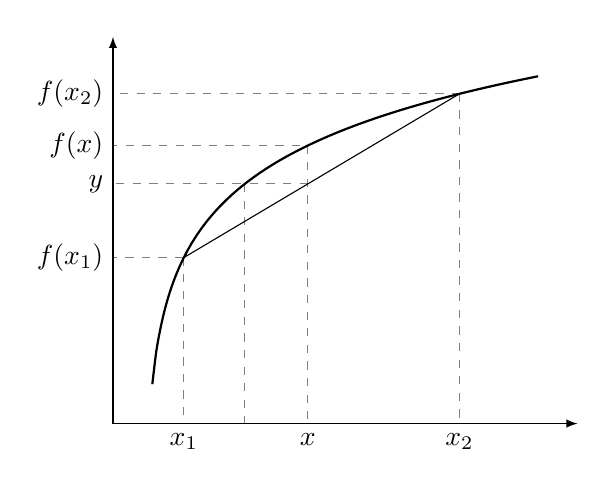
\begin{tikzpicture}[my plot/.style={
                        thick,
                        smooth,
                        samples=100,
                        domain=0.1:5},
                    my grid/.style={dashed,opacity=0.5, every node/.style={black,opacity=1}},
                    my axis/.style={latex-latex}]
\draw[my plot] (0,0) plot (\x,{ln(\x)});
\coordinate (start plot) at (0.1,{ln(0.1)}); % domain start
\coordinate (end plot) at (5,{ln(5)}); % domain end
\draw[my axis] ([shift={(-0.5cm,0.5cm)}]start plot |- end plot) node[left] {} |- node[coordinate](origin){} ([shift={(0.5cm,-0.5cm)}]start plot -| end plot) node[below] {}; %creates the axis a little bigger than the plot and also sepatared
\def\x{0.5}\def\y{4}\def\p{0.55} % define the x, y and p values
\coordinate (Ux) at (\x,{ln(\x)}); % set the u(x) coordinate
\coordinate (Uy) at (\y,{ln(\y)}); % set the u(y) coordinate
\coordinate (Up) at ({\p*\x+(1-\p)*\y},{ln(\p*\x+(1-\p)*\y)}); % set the u(p*x+(1-p)*y) coordinate
\draw (Ux) -- coordinate[pos=1-\p] (Up-mid) (Uy); % set the coordinate on the linear curve
\path let \p1=(Up-mid), \n1={pow(e,\y1*0.03514)} in (28.4576*\n1,\y1) coordinate (Up-mid2); %this is the most tricky part explained in the answer
% with everything set, just draw the lines:
\draw[my grid] (Ux) |- node[below]{$x_1$} (origin) |- node[left]{$f(x_1)$} cycle;
\draw[my grid] (Uy) |- node[below]{$x_2$} (origin) |- node[left]{$f(x_2)$} cycle;
\draw[my grid] (Up) |- node[below]{$x$} (origin) |- node[left]{$f(x)$} cycle;
\draw[my grid] (Up-mid2) |- node[below]{} (origin) |- node[left]{$y$} cycle;
\draw[my grid] (Up-mid) -- (Up-mid2);
\end{tikzpicture}
\end{center}
\end{annotation}


\begin{annotation}
\rm 我们这里使用的凹凸性都是描述函数性质的,并不是用来描述函数图像的,{\color{red}高数书使用的是对图像的凹凸性描述的},这里有几种记忆函数凹凸性质的方法.
\begin{enumerate}
	\item 从几何性质上,凹函数的曲线在两点确定的弦之上,凸函数的曲线在两点确定的弦之下.
\end{enumerate}	
\end{annotation}

\begin{theorem}
\rm {\color{red} (凹凸性判定1)} 给定在区间$\mathcal{X}$上定义着的连续可导函数$f(x)$,它是凸函数(凹函数)当且仅当它导数$f'(x)$是单调增的(单调减的). 
\end{theorem}

\begin{proof}
前面我们知道凸函数的性质可以用
$$
f(x) \leq \frac{x_2 - x}{x_2-x_1}f(x_1) + \frac{x-x_1}{x_2-x_1}f(x_2),\; x \in [x_1,x_2]
$$
来描述,来略微整理一下
$$
\begin{array}{ll}
&(x_2-x)f(x_1) + (x_1-x_2)f(x) + (x-x_1)f(x_2) \geq 0 \\ \\
\Rightarrow & (x_2 - x)(f(x_1)-f(x)) + (x_1 -x)(f(x)-f(x_2)) \leq  0 \\ \\
\Rightarrow & \frac{f(x) - f(x_1)}{x -x_1} \leq \frac{f(x_2) - f(x)}{x_2 - x} \\
\end{array}
$$
不等式两边在必要性证明中可以让$x$分别趋向$x_1$或者$x_2$求得
$$
f'(x_1) \leq \frac{f(x_2) - f(x_1)}{x_2 - x_1}
$$
和 
$$
f'(x_2) \geq \frac{f(x_2) - f(x_1)}{x_2 - x_1} 
$$
即有$f'(x_2) \geq f(x_1)$.

在充分证明中可以使用拉格朗日中值定理让等式两边分别等于$f(\xi_1)$和$f(\xi_2)$,其中$x_1 < \xi_1 < x < \xi_2 < x_2$.
\end{proof}


\begin{theorem}
\rm {\color{red} (凹凸性判定2)} 给定在区间$\mathcal{X}$上定义着的连续且二阶可导函数$f(x)$,它是凸函数(凹函数)当且仅当$f^{''}(x) \geq 0(\leq 0)$.
\end{theorem}

\begin{proof}
由单调性判定定理,回到前一个定理中的$f'(x)$的性质即可.
\end{proof}

\begin{theorem}
\rm {\color{red} (凹凸性判定3)} 给定在区间$\mathcal{X}$上定义着的连续可导函数$f(x)$,它是凸函数(凹函数)当且仅当它的曲线在它任意切线上面(切线下面).
\end{theorem}

\begin{proof}
{\color{blue}充分性} 任意点$x_0 \in \mathcal{X}$处切线方程$y = f(x_0) + f'(x)(x-x_0)$,那么只需要证明
$$
f(x) \leq f(x_0) + f'(x)(x-x_0) 
$$
当$x > x_0$时有
$$
f'(x_0) \geq \frac{f(x)-f(x_0)}{x-x_0}.
$$
当$x < x_0$时有
$$
f'(x_0) \leq \frac{f(x)-f(x_0)}{x-x_0}.
$$
那么根据拉格朗日中值定理可以找到$\xi_1 <x_0 < \xi_2$,使得
$$
f'(x_0) \leq f'(\xi_2),\; f'(x_0) \leq f'(\xi_1).
$$
即$f'(\xi_1) \leq f'(\xi_2)$,回到第一个判别定理.
\end{proof}

\begin{proposition}
\rm {\color{red} (琴生不等式)} 凸函数满足 
$$
f(q_1x_1 + q_2x_2 + \cdots + q_nx_n) \leq q_1f(x_1) +q_2f(x_2) + \cdots + q_nf(x_n),
$$
其中$q_1 + q_2 + \cdots + q_n = 1,\; q_1,q_2,\cdots,q_n > 0$.
\end{proposition}

\begin{definition}
\rm 若曲线$f(x)$在经过$(x_0,f(x_0))$时,曲线的凹凸性改变了,则这一点称为{\color{red}拐点}.
\end{definition}

\begin{proposition}
\rm {\color{red}判别拐点的存在方法}
\begin{enumerate}
	\item 若$f(x)$的二阶导存在,且$f(x)$在$x_0$处$f^{''}(x)=0$变号,则在$x_0$处有拐点.
	\item 若$f(x)$的$n$阶导数存在,如果点$x_0$处第一个不为零的导数(大于二阶导)是奇数阶导数,那么在$x_0$处有拐点,如果是偶数阶导数,则没有拐点.
\end{enumerate}
\end{proposition}

\newpage
\section{不定积分}

\subsection{不定积分定义}
\begin{definition}
\rm 若在给定的整个区间上,$f(x)$是函数$F(x)$的导数,或$f(x)dx$是$F(x)$的微分,即
$$
F'(x) = f(x)~\text{或}~dF(x) = f(x)dx,
$$
那么,在所给定的区间上,函数$F(x)$叫做$f(x)$的{\color{red}原函数}或者$f(x)$的{\color{red}积分}.
\end{definition}

\begin{theorem}
\rm {\color{red} (不定积分表达式) }若在某一个区间$\mathcal{X}$上,函数$F(x)$是$f(x)$的一个原函数,那么$F(x)+C$也是$f(x)$的原函数,其中$C$是任意常数. 反过来说,在区间$\mathcal{X}$上$f(x)$的每一个原函数都可表示这种形式.
\end{theorem}

\begin{proof}
记$\Phi(x)$是$f(x)$另一个原函数,则考虑辅助函数$\varphi(x) = \Phi(x) - F(x)$的导数
$$
(\Phi(x)-F(x))' = f(x)-f(x) = 0.
$$
由常函数判定定理,可以知道$\varphi(x) = C$,所以$\Phi(x) = F(x) + C$.
\end{proof}

\begin{definition}
\rm 在区间$\mathcal{X}$,函数$f(x)$的带任意常数项的原函数称为$f(x)$在$\mathcal{X}$上的{\color{red}不定积分},记做
$$
\int f(x)dx
$$
来表示,其中$f(x)$表示{\color{red}被积函数},乘积$f(x)dx$被称为{\color{red}被积表达式}.
\end{definition}

\begin{proposition}
\rm 从不定积分的定义可以很容易直接推导下面一些性质
\begin{enumerate}
	\item $d\int f(x)dx = f(x)dx,$
	\item $\int F'(x)dx = F(x)+C~\text{或}~\int dF(x) = F(x)+C.$
\end{enumerate}
\end{proposition}

\begin{theorem}
\rm \redt{原函数的存在性} 在给定区间上的每个连续函数$f(x)$都有在这区间上的原函数.
\end{theorem}

\begin{theorem}
\rm 若$f(x)$在给定区间上有第一类间断点,则$f(x)$没有原函数. 若有第二类间断点,可能有原函数也可能没有.  
\end{theorem}

\begin{proof}
有第一类间断点意味着在那一点左右导数不一样的,这个地方就是不可导的. 
\end{proof}

\newpage
\subsection{基本积分表}

\begin{proposition}
\rm \
\begin{enumerate}
	\item $\int 0dx = C$
 	\item $\int x^{\alpha}dx = \frac{1}{\alpha+1}x^{\alpha+1}~(\alpha \neq 0)$ 
	\item $\int \frac{1}{x} dx = \ln |x| + C$
	\item $\int a^{x}dx = \frac{a^x}{\ln a} + C$
	\item $\int e^x dx = e^x + C$
	\item $\int \sin x dx = -\cos x + C$
	\item $\int \cos x dx = \sin x + C$
	\item $\int \sec^2 x dx = \tan x +C$
	\item $\int \csc^2 x dx = -\cot x + C$
	\item $\int \sec x\tan x dx = \sec x +C$
	\item $\int \csc x\cot x dx = -\csc x + C$
	\item $\int \frac{1}{\sqrt{1-x^2}}dx = \arcsin x+C$
	\item $\int \frac{1}{1+x^2}dx = \arctan x + C$
	\item $\int \frac{1}{\sqrt{a^2 -x^2}} = \arcsin \frac{x}{a} + C$
	\item $\int \frac{1}{a^2 + x^2}dx = \frac{1}{a}\arctan \frac{x}{a} + C$
	\item $\int \frac{1}{x^2 - a^2} =\frac{1}{2a} \ln \left| \frac{x-a}{x+a}\right|+C$
	\item $\int \frac{1}{\sqrt{x^2 + a^2}}dx = \ln(x+\sqrt{x^2 + a^2})+C$
	\item $\int \frac{1}{\sqrt{x^2 - a^2}}dx = \ln \left| x+ \sqrt{x^2 - a^2}\right|+C$
	\item $\int \sec x dx = \ln |\sec x + \tan x|+C$
	\item $\int \csc x dx = -\ln|\csc x + \cot x|+C$
\end{enumerate}
\end{proposition}

\subsection{高次积分}

\begin{proposition}
\rm 常用的高次积分降次公式
\begin{enumerate}
	\item $\int \cos ^{n}(x)\,dx={\frac  {1}{n}}\cos ^{{n-1}}(x)\sin(x)+{\frac  {n-1}{n}}\int \cos ^{{n-2}}(x)\,dx$;
	\item $\int \sin ^{n}(x)\,dx=-{\frac  {1}{n}}\sin ^{{n-1}}(x)\cos(x)+{\frac  {n-1}{n}}\int \sin ^{{n-2}}(x)\,dx$;
	\item $\int \tan ^{n}(x)\,dx={\frac  {1}{n-1}}\tan ^{{n-1}}(x)-\int \tan ^{{n-2}}(x)\,dx$;
	\item $\int (\ln(x))^{n}\,dx=x(\ln(x))^{n}-n\int (\ln(x))^{{n-1}}\,dx$.
\end{enumerate}
\end{proposition}

\subsection{简单积分法则}

\begin{proposition}
\rm 简单法则
\begin{enumerate}
	\item 若$a$是常数且不等于0,则
	$$
	\int a\cdot f(x)dx = a \int f(x)dx,
	$$
	\item 
	$$
	\int \left[ f(x) \pm  g(x) \right]dx = \int f(x)dx + \int g(x)dx,
	$$
	\item 若$\int f(t)dt = F(t)+C$,则
	$$
	\int f(ax+b)dx = \frac{1}{a}\cdot F(ax+b)+C'
	$$
	{\color{red} 换元法则中极为特别的情形}
\end{enumerate}
\end{proposition}

\begin{proof}
{\color{blue}证明手法通常对右边取微分}.
\end{proof}


\subsection{换元积分法}
\begin{proposition}
\rm 如果已知
$$
\int g(t)dt = G(t)+C,
$$
即有
$$
\int g(\omega(x))\omega'(x)dx = G(\omega(x)) + C'.
$$
其中$\omega(x)$有连续的导函数. 
\end{proposition}

\begin{proof}
$$
\frac{d}{dx}G(\omega(x)) = G'(\omega(x))\omega'(x) = g(\omega(x))\omega'(x).
$$
\end{proof}

\begin{annotation}
\rm {\color{red} (换元积分法使用的直觉)} 要理解上述方法的先决条件,只需要关系式$dG(t)=g(t)dt$成立,就有上述换元之后的关系式存在. 现在换个思路,若先要计算积分
$$
\int f(x)dx,
$$
但是这个$f(x)$并不好直接利用现有的一些手法求出其原函数,若被积部分可以表示成前面第二个关系式的左边
$$
f(x)dx = g(\omega(x))\omega'(x)dx,
$$
那么说明其原函数可以表示$G(\omega(x))$,这样我们尝试先求出$G(t)$,现在我们让$t=\omega(x)$,上式就变成了$\int g(t)dt$,{\color{blue}最重要是需要它是可以稍微容易求解原函数的$g(t)$形式,不然换元就没什么意义}. 那么把它积出来之后等于$G(t)+C$,之后我们只需要把$t$用$\omega(x)$替换即可.
\end{annotation}

\begin{example}
\rm 求积分
$$
\int \sin^3\cos xdx.
$$
设$t=\sin x$,那么原式为
$$
\int \sin^3x\cos xdx = \int \sin^3xd\sin x = \int t^3 dt = \frac{t^4}{t}+C.
$$
最后$t$替换为$\sin x$即可.
\end{example}

\begin{proposition}
\rm 已知$f(x)$的原函数凑微分常用手法
\begin{enumerate}
	\item $\int f(ax+b)dx = \frac{1}{a} \int f(ax+b)d(ax+b)$
	\item $\int x^m f(ax^{m+1}+b)dx = \frac{1}{(m+1)a}\int f(ax^{m+1}+b)d(ax^{m+1}+b)$
	\item $\int \frac{f(\sqrt{x})}{\sqrt{x}}dx = 2 \int f(\sqrt{x})d\sqrt{x}$
	\item $\int f(e^x)e^xdx = \int f(e^x)de^x$
	\item $\int \frac{f(\ln x)}{x}dx = \int f(\ln x)d\ln x$
	\item $\int f(\sin x)\cos x dx = \int f(\sin x)d\sin x$
	\item $\int f(\cos x)\sin x dx = -\int f(\cos x)d\cos x$
	\item $\int \frac{f(\tan x)}{\cos^2 x}dx = \int f(\tan x)d \tan x$
	\item $\int \frac{\arcsin x}{\sqrt{1-x^2}}dx = \int f(\arcsin x)d\arcsin x$
	\item $\int \frac{\arctan x}{1+x^2}dx = \int f(\arctan x) d\arctan $
\end{enumerate}
\end{proposition}

\begin{proposition}
\rm \redt{第二类换元法} 设$x = \varphi(t)$是单调的,可导的函数,并且$\varphi'(t) \neq 0$. 若
$$
\int f[\varphi(t)]\varphi'(t)dt = F(t)+C,
$$
则
$$
\int f(x)dx = \int f[\varphi(t)]\varphi'(t)dt = F(t) + C = F[\varphi^{-1}(x)]+C,
$$
其中$\varphi^{-1}(x)$是$x=\varphi(t)$的反函数. 
\end{proposition}

\begin{example}
\rm 求积分
$$
\int \frac{1}{\sqrt{x}(1+\sqrt[3]{x})}dx
$$
这里令$x=t^3$,那么原式就变成了
$$
\int \frac{6t^5}{t^3(1+t^2)}dt = 6\int \left[ 1-\frac{1}{1+t^2} \right] = 6t-6\arctan t + C = 6\sqrt[6]{x}-6\arctan \sqrt[6]{x} + C
$$
\end{example}

\begin{proposition}
\rm 常见$x$用$\varphi(t)$做变量代换
\begin{enumerate}
	\item 被积函数含有$\sqrt{a^2-x^2}$,令$x=a\sin t$或者$x=a\cos t$.
	\item 被积函数含有$\sqrt{a^2 + x^2}$,令$x=a\tan t$.
	\item 被积函数含有$\sqrt{x^2-a^2}$,令$x=a\sec t$. 
\end{enumerate}
\end{proposition}

\subsection{分部积分法}

\begin{proposition}
\rm 设$u=f(x)$和$v=g(x)$都是两个关于$x$的连续可导的函数,则
$$
\int udv  = uv - \int vdu.
$$
\end{proposition}

\begin{proof}
根据微分乘法法则
$$
d(uv) = udv + udv,
$$
两边取积分得到原式.
\end{proof}

\begin{annotation}
\rm {\color{red} (分部积分使用注意)} 它进行如下转换
$$
f(x)dx = uv'dx = udv = uv-vdu = vu'dx.
$$
在应用分部积分的时候,需要注意以下几点
\begin{enumerate}
	\item 被积表达式$f(x)$要被分成两个因式$u$和$dv=v'dx$.
	\item 微分$vu'dx$要比原式更容易积分.
\end{enumerate}
\end{annotation}


\begin{example}
\rm 求积分
$$
\int x\cos xdx.
$$
设$u=x,\; v= \sin x$,那么原式变为
$$
\int xd\sin x = x\sin x - \int \sin x dx = x\sin x +\cos x + C.
$$
\end{example}

\begin{proposition}
\rm 常用部分积分法中$u,v$的选取
\begin{enumerate}
	\item 把多项式以外的函数凑集微分符号里面
	$$
	\int p_n(x)e^{ax}dx, \int p_n(x)\sin \alpha xdx,\int p_n\cos xdx.
	$$
	\item 把指数函数凑进微分符号
	$$
	\int e^{\alpha x}\sin\beta x dx, \int e^{\alpha x}\cos \beta x dx.
	$$
	\item 把多项式凑进微分符号
	$$
	\int p_n(x)\ln x dx, \int p_n(x)\arctan x dx, \int p_n(x)\arcsin x dx. 
	$$
\end{enumerate}
\end{proposition}

\begin{proposition}
\rm {\color{red} (分部积分的推广公式)} 若$u$和$v$在所考虑的区间上有直到$(n+1)$阶的各阶连续导数,那么可以用$v^{(n)}$替换前式中的$v$,则
$$
\int uv^{(n+1)}dx = \int udv^{(n)} = uv^{(n)} - \int v^{(n)}du = uv^{(n)} - \int u'v^{(n)}dx.
$$
类似的
$$
\begin{array}{ll}
\int u'v^{(n)}dx &= u'v^{(n-1)} - \int u^{''}v^{(n-1)}dx, \\
\int u^{''}v^{(n-1)}dx &= u^{''}v^{(n-2)} - \int u^{'''}v^{(n-2)}dx, \\
&\vdots \\
\int u^{(n)}v'dx &= u^{(n)}v - \int u^{(n+1)}vdx, \\
\end{array}
$$
因此最终可以得到
$$
\int uv^{(n+1)}dx = uv^{(n)} - u'v^{(n-1)} + u^{''}v^{(n-2)} -\cdots + (-1)^{n} u^{(n)}v +  (-1)^{n+1} \int u^{(n+1)}vdx.
$$
\end{proposition}

\begin{annotation}
\rm {\color{red} (推广式中的特殊情况) }特别地,如果$u$是$n$元多项式,那么在$n+1$次求导之后就变成零了,上式子的尾巴就消失了.
\end{annotation}

\begin{example}
\rm 求积分
$$
J_n = \int \frac{1}{(x^2+a^2)^n}dx,\; n =1,2,3,\cdots.
$$
令$u=\frac{1}{(x^2+a^2)^n},\; v = x$,即
$$
J_n = \int \frac{1}{(x^2+a^2)^n}dx = \frac{x}{(x^2+a^2)^n} + 2n \int \frac{x^2}{(x^2+a^2)^{n+1}}dx. 
$$
考虑右式最后一项
$$
\int \frac{x^2}{(x^2+a^2)^{n+1}}dx =\int \frac{(x^2+a^2) - a^2}{(x^2+a^2)^{n+1}}dx = J_n - a^2 J_{n+1}.
$$
带入原式
$$
J_n = \frac{x}{(x^2+a^2)^n}+2nJ_n - 2a^2nJ_{n+1},
$$
整理得到{\color{red}递归式}
$$
J_{n+1} = \frac{1}{a^2}\frac{2n-1}{2n}J_n + \frac{1}{2a^2}\frac{1}{n}\frac{x}{(x^2+a^2)^n}.
$$
易得$J_1 = \frac{1}{a} \arctan \frac{x}{a}.$ 
\end{example}

\subsection{有理式积分}

\begin{annotation}
\rm 在各类函数的积分中使我们{\color{red}最感兴趣的是什么},要根据什么样的{\color{red}法则},才能得到它们的积分,是这一节我们主要关注的问题. 积佬养成)
\end{annotation}

\begin{definition}
\rm 形如
$$
f(x)=\frac{P(x)}{Q(x)}
$$
的函数,其中$P(x),Q(x)$均为多项式. 这样的函数被称为{\color{red}有理函数}.
\end{definition}

\begin{proposition}
\rm 两种{\color{red}简单真分式}积分方法
\begin{enumerate}
	\item $\frac{A}{x-a}$
	$$
	A\int \frac{1}{x-a}dx = A \ln(x-a) + C.
	$$
	\item $\frac{A}{(x-a)^k},\; k = 2,3,\cdots$
	$$
	A\int \frac{1}{(x-a)^k}dx = -\frac{A}{k-1}\frac{1}{(x-a)^{k-1}} + C
	$$
\end{enumerate}
\end{proposition}

\begin{annotation}
\rm {\color{red}(部分分式)}求积分
$$
\int \frac{Mx+N}{(x^2+px+q)^m}dx,\; m = 2,3,4,\cdots.
$$
同时假定$x^2+px+q$没有实根,即$p^2 - 4q < 0$.

先对分母括号中的二次多项式进行配方
$$
\begin{array}{ll}
\int \frac{Mx+N}{(x^2+px+q)^m}dx &= \int \frac{Mx+N}{(x^2+2\frac{p}{2}x+\frac{p^2}{4}-\frac{p^2}{4}+q)^m}dx\\
&= \int \frac{Mx+N}{\left[(x+\frac{p}{2})^2+(q-\frac{p^2}{4})\right]^m}dx
\end{array}
$$
设$x+\frac{p}{2} = t, a = + \sqrt{q-\frac{p^2}{4}}$,现在$dt=dx$,那么原式变为
$$
\int \frac{M(t-\frac{p}{2})+N}{\left(t^2+a^2\right)^m}dt = M\int \frac{t}{\left(t^2+a^2\right)^m}dt + (N-\frac{Mp}{2})\int \frac{1}{\left(t^2+a^2\right)^m}dt,
$$
等式右边第一个积分,设$t^2+a^2 = u$,那么其积分变为
$$
M\int \frac{t}{\left(t^2+a^2\right)^m}dt = \frac{M}{2} \int  \frac{du}{u^m} = \frac{M}{2} \frac{-1}{m-1}\frac{1}{u^{m-1}} + C = \frac{-M}{2(m-1)}\frac{1}{(t^2+a)^{m-1}}+C.
$$
右边第二个积分使用我们在分部积分里面提到的{\color{blue}递归式求解}即可. 
\end{annotation}

\begin{theorem}
\rm 每个真分式
$$
\frac{P(x)}{Q(x)}
$$
可被表示成{\color{red}有限个部分分式的代数和}的形状. {\color{blue}总感觉有点环上PID性质在里面??????}
\end{theorem}

\begin{proof}
首先我们需要知道任意一个多项式的分解可以写成下述形式
$$
Q(x) = (x-a)^k \cdots (x^2+px+q)^m \cdots,\; k,m \in \mathbb{N},\; a,p,q \in \mathbb{R},
$$
其中$x^2+px+q$没有实根,相当于在实数环上做因式分解. 下面分两种情况来讨论$\frac{P(x)}{Q(x)}$的部分分式. 

{\color{blue}(1)} 若所给真分式为
$$
\frac{P(x)}{Q(x)} = \frac{P(x)}{(x-a)^kQ_1(x)}.
$$
则可以表示成下述两个真分式的和
$$
\frac{P(x)}{(x-a)^kQ_1(x)} = \frac{A}{(x-a)^k} + \frac{P_1(x)}{(x-a)^{k-1}Q_1(x)},
$$
其中$A$是一个常量,接下来就是确定$A$和$P_1(x)$,即这里有一个恒等式
$$
P(x) = AQ_1(x) + P_1(x)(x-a).
$$
首先我们得确定这里有解才行,{\color{blue}注意这里$(x-a)$和$Q_1(x)$是互素的,但是不能直接用Bezout定理说明这里有解,因为这里限定$A$是一个常量而不是一个关于$x$的多项式}. 那么现在问题变成了要说明其中一个解是常量,是这样的因为Bezont定理,我们得到这样一个等式
$$
u(x)Q_1(x) + v(x)(x-a) = 1.
$$
可以来尝试把所有$Q_1(x)$和$(x-a)$线性组合为$1$的系数用已知的$u(x)$和$v(x)$表示出来,即
$$
U(x) = u(x) - (x-a)t(x),\; V(x) = v(x) + Q_1(x)t(x). 
$$
我们主要关注$U(x)$来说明一定可以取到常数$A$,相当于$U(x)$可以是$u(x)$除$(x-a)$的余数,所以$U(x)$是一定可以取到某个常数$A$.自然地,这里考虑可以取$x = a$消去含$P_1(x)$的项,于是得到$A=\frac{P(a)}{Q_1(a)}$,随之再确定$Q_1(a)$. 记录一个我自己的疑问{\color{red}为什么给定真分式不能分解为}
$$
\frac{A}{(x-a)^k} + \frac{B}{Q_1(x)},\; k=2,3,\cdots,
$$
那么确定的恒等式就变成了
$$
P(x) = AQ_1(x) + B(x-a)^k, 
$$
按照前面的思路这里$U(x) = u(x) - (x-a)^kt(x)$,所以只能保证$U(x)$取到某个$a_{k-1}x^{k-1}+a_{k-2}x^{k-2}+\cdots+a_0$,那么这里$A$可能就不一定是一个常数.

{\color{blue}(2)} 若所给真分式为
$$
\frac{P(x)}{Q(x)} = \frac{P(x)}{(x^2+px+q)^mQ_1(x)}.
$$
则可以表示成下述两个真分式的和
$$
\frac{P(x)}{(x+px+q)^mQ_1(x)} = \frac{Mx+N}{(x^2+px+q)^m} + \frac{P_1(x)}{(x^2+px+q)^{m-1}Q_1(x)}.
$$
其中$M,N,P_1(x)$确定要稍微复杂一点,但是整体思路是明确的,详细参考菲砖对应有理分式积分章节.

上面两种情况的尾巴均可以再依次取类似的部分分式,即
$$
\frac{A_1}{x-a} + \frac{A_2}{(x-a)^2} + \cdots + \frac{A_k}{(x-a)^k}.
$$
和
$$
\frac{M_1x+N_1}{x^2+px+q} + \frac{M_2x+N_1}{(x^2+px+q)^2} + \cdots + \frac{M_{m}x+N_{m}}{(x^2+px+q)^m}.
$$
对其部分分式代数和进行积分将比原始要简单的多! 但是这里只是证明某个真分式可以被表示成有限个部分分式,但是具体相关的系数其实都只是指称,若展开成代数和形式之后,求相关的系数方法,我们称其为{\color{red}待定系数法}.
\end{proof}


\begin{example}
\rm 求下列给定分式的分解式
$$
\frac{2x^2+2x+13}{(x-2)(x^2+1)^2}
$$
原式的分解形式可以先写成如下形式
$$
\frac{A}{x-2} + \frac{Bx+C}{x^2+1} + \frac{Dx+E}{(x^2+1)^2}.
$$
其中$A,B,C$就是待定系数,它和原式关系等式为
$$
\begin{array}{ll}
2x^2 + 2x+ 13 &= A(x^2+1)^2 + (Bx+C)(x-2)(x^2+1) + (Dx+E)(x-2) \\
			  &= (A+B)x^4 + (C-2B)x^3 + (2A+B-2C+D)x^2 + (C-2B-2D+E)x + (A-2C-2E).
\end{array}
$$
这里对应一个含5个方程的方程组
$$
\left\{ 
\begin{array}{ll}
A+B &= 0 \\
C-2B &= 0 \\
2A+B-2C+D &= 2 \\
C-2B-2D+E &= 2 \\
A-2C-2E &= 13  
\end{array}
\right.
$$
解这个方程组可以先利用后三项消去$D,F$得到一个只含$A,B,C$的等式,再配合前两项,先解出$A,B,C$. 由此
$$
A = 1,\;B = -1,\;C = -2,\;D = -3 ,\;E=-4.
$$
最后
$$
\frac{2x^2+2x+13}{(x-2)(x^2+1)^2} = \frac{1}{x-2} + \frac{-x-2}{x^2+1} + \frac{-3x-4}{(x^2+1)^2}.
$$
\end{example}

\subsection{三角有理式}

\begin{proposition}
\rm \redt{万能公式} 令$t = \tan \frac{x}{2}$,
$$
\int R(\sin x , \cos x)dx = \int R\left(\frac{2t}{1+t^2},\frac{1-t^2}{1+t^2}\right)\frac{2}{1+t^2}dt,
$$
其中$R(\sin x , \cos x)$表示自变量为$\sin x,\cos x$的有理函数.
\end{proposition}

\begin{proof}
根据三角函数中的万能公式
$$
\begin{array}{ll}
\sin x = \frac{2\tan \frac{x}{2}}{1+\tan^2\frac{x}{2}} = \frac{2t}{1+t^2} \\
\cos x = \frac{1-\tan^2 \frac{x}{2}}{1+\tan^2\frac{x}{2}} = \frac{1-t^2}{1+t^2} \\
\end{array}
$$
而$x = 2\arctan t$,所以$dx = \frac{2}{1+t^2}dt$. 
\end{proof}

\begin{proposition}
\rm 给定多项式$p_n(x)=a_0 + a_1x^1 + \cdots a_{n}x^n$,若$p_n(x) = p_n(-x)$,则
$$
p_n(x) = p_n^*(x^2).
$$
\end{proposition}

\begin{proof}
若$p_n(x) = p_n(-x)$,则
$$
p_n(x) - p_n(-x) = 2a_1x + \cdots + 2a_{2m-1}x^{2m-1} = 0.
$$
因此
$$
q_{n-m}(x) = a_1x + \cdots + a_{2m-1}x^{2m-1} = 0,
$$
那么
$$
p_n(x) = a_0 + a_2x^{2} + \cdots + a_{2m}x^{2m}  + q_{n-m}(x)
$$
显然$p_n(x) = p_n^*(x^2)$. 
\end{proof}

\begin{proposition}
\rm $p_n(x)=a_0 + a_1x + \cdots a_{n}x^n$,若$p_n(x) = -p_n(-x)$,则
$$
p_n(x) = p_n^{**}(x^2)x.
$$
\end{proposition}

\begin{proof}
若$p_n(x) = -p_n(-x)$,那么
$$
p_n(x) + p_n(-x) = 2a_0 + 2a_2x^{2} +\cdots + 2a_{2m}x^{2m} = 0.
$$
因此
$$
q_{n-m-1}(x) = a_0 + a_2x^2 + \cdots +a_{2m}x^{2m}=0.
$$
于是
$$
p_n(x) = a_1x + \cdots + a_{2m-1}x^{2m-1} + q_{n-m-1}(x).  
$$
显然
$$
p_n(x) = p_n^{**}(x^2)x
$$
\end{proof}

\begin{corollary}
\rm 如果
$$
R(-u,v) = R(u,v),
$$
则这个有理函数可以化为只含$u$的偶次幂的形状
$$
R(u,v) = R_1(u^2,v).
$$
如果
$$
R(-u,v) = -R(u,v),
$$
则这个有理函数可以化为
$$
R(u,v) = R_2(u^2,v)u.
$$
\end{corollary}

\begin{corollary}
\rm 如果
$$
R(-u,-v) = R(u,v),
$$
则
$$
R(u,v) = R_3(\frac{u}{v},v^2).
$$
\end{corollary}

\begin{proposition}
\rm 特殊凑微分方法
\begin{enumerate}
	\item 若$R(-\sin x,\cos x) = - R(\sin x, \cos x)$,此时
	$$
	R(\sin x,\cos x)dx = R_2(\sin^2 x, \cos x)\sin x dx = -R_0(1-\cos^2x,\cos x)d\cos x.
	$$
	\item 若$R(\sin x,-\cos x) = - R(\sin x, -\cos x)$,此时
	$$
	R(\sin x,\cos x)dx = R_2^*(\sin x, \cos^2x )\cos x dx = -R_0^*(\sin x , 1-\sin^2 x)dsinx.
	$$
	\item 若$R(-\sin x, -\cos x) = R(\sin x ,\cos x)$ 
	$$
	R(\sin x, \cos x)dx = R_3(\tan x,\cos^2 x)dx = R_3(\tan x, \frac{1}{1+\tan^2 x})dx,
	$$
	令$t = \tan x$,则有
	$$
	R(\sin x, \cos x)dx = R\left(t,\frac{1}{1+t^2}\right)\frac{1}{1+t^2}dt. 
	$$
\end{enumerate}
\end{proposition}

\subsection{根式有理式}

\begin{proposition}
\rm \redt{根式有理化} 形如
$$
\int R(x,\sqrt[n]{\frac{ax+b}{cx+d}})
$$
的积分,令$t = \sqrt[n]{\frac{ax+b}{cx+d}}$,那么$x = \varphi(t) = \frac{b-t^nd}{t^nc -a}$,则
$$
\int R(\varphi(t),t)\varphi'(t)dt
$$
就变成了有理函数的形状. 
\end{proposition}

\begin{example}
\rm 求
$$
\int \frac{1}{x} \sqrt{\frac{x+1}{x}}dx.
$$
令$t = \sqrt{\frac{x+1}{x}}$,那么$x=\frac{1}{t^2-1}, dx = \frac{-2t}{(t^2-1)^2}$,于是
$$
\int (t^2 - 1) t \frac{-2t}{(t^2-1)^2} dt = -2\int \frac{t^2}{(t^2-1)}dt = -2 \int 1  + \frac{1}{t^2-1}dt = -2(t  + \frac{1}{2}\ln \left| \frac{t-1}{t+1} \right|) + C. 
$$
\end{example}

\newpage
\section{定积分}

\subsection{定积分定义}

\begin{definition}
\rm 给定定义在区间$[a,b]$上的函数$f(x)$. 在$a$和$b$之间插入若干分点
$$
a = x_0 < x_1 <x_2 < \cdots < x_{n-1} < x_n = b
$$
把$[a,b]$分成$n$个小区间
$$
[x_0,x_1],[x_1,x_2],\cdots,[x_{n-1},x_n].
$$
用$\Delta x_i = x_{i+1}-x_i$第$i$小区间的长度,记$\lambda = \max{\{\Delta x_i\}}$. 从每个小区间$[x_i,x_{i+1}]$上任取一点$x=\xi_i$并做出和
$$
\sigma = \sum\limits_{i=0}^{n-1}f(\xi_i)\Delta x_i.
$$
若$\lambda \rightarrow 0$时$\sigma$有有限极限$I$,用极限的语言描述即对任意的$\varepsilon > 0$,都可以找到数$\delta$,只要$\lambda < \delta$,不等式
$$
|\sigma - I| < \varepsilon
$$
在任意的$\xi_i$选择之下皆成立,把其记做
$$
I = \lim\limits_{\lambda \rightarrow 0} \sigma.
$$
则这极限$I$叫做函数$f(x)$在从$[a,b]$上的{\color{red}定积分},记为
$$
I = \int_a^b f(x)dx.
$$
在这情形下$f(x)$叫做$[a,b]$上的{\color{red}可积函数},数$a$与$b$分别叫做积分的{\color{red}上限}和{\color{red}下限},区间$[a,b]$,叫做{\color{red}积分区间},变量$x$叫做{\color{red}积分变量}. $\sigma$也被称为{\color{red}黎曼和},上述定义本身就是{\color{red}黎曼定义}.
\end{definition}

\subsection{定积分基本性质}

\begin{proposition}
\rm {\color{red} (可积的必要条件)} $f(x)$在$[a,b]$上可积,则$f(x)$在$[a,b]$上有界.
\end{proposition}

\begin{proof}
若$f(x)$在$[a,b]$上可积,假设$f(x)$在$[a,b]$上无界,那么对于黎曼和的求法,无论怎样划分区间,都有一部分区间无界. 于是靠着这个区间的$\xi$的选择,对应$f(\xi)$可以任意大或者任意小,那么$\sigma$也是随之任意大或任意小. 这样导致$\sigma$是不可能存在有限极限的. 
\end{proof}

\begin{definition}
\rm 用$m_i$与$M_i$分别表示函数$f(x)$在第$i$个部分区间$[x_i,x_{i+1}]$上的下确界和上确界,并作和
$$
s = \sum\limits_{i=0}^{n-1}m_i\Delta x_i,\; S = s = \sum\limits_{i=0}^{n-1}M_i\Delta x_i
$$
这两个和分别叫做{\color{red}下积分}和与{\color{red}上积分和},或者{\color{red}达布和}. 当$f(x)$连续时,$f(x)$在每个区间上都能去掉确界,于是
$$
m_i \leq f(\xi_i) \leq M_i,
$$ 
自然地也有
$$
s \leq \sigma \leq S.
$$
这意味着$s$与$S$分别是积分和的下确界与上确界.
\end{definition}


\begin{lemma}
\rm 如果把一些新的点加入到已有的分点中,即插入$x'$位于任意的部分区间$[x_k,x_{k+1}]$有$x_k < x' < x_{k+1}$. 则达布下和只有可能因此增加,而上和只可能减少.
\end{lemma}

\begin{proof}
一个小区间被分成了两个更小的区间,这两个更小区间的积分和加起来是小于原先区间的积分和.
\end{proof}

\begin{lemma}
\rm 任何一个达布下和都不超过任何一个上和,即使是对应于区间的另一个划分的上和,即两个不同的区间划分构造$s_1,S_2$和$s_2,S_2$,也有$s_1 < S_2$.
\end{lemma}

\begin{proof}
通过第一个lemma,通过加点的方式,联合两个构造组成一个新的构造$s_3,S_3$,因此有$s_1 \leq s_3$和$S_2 \geq S_3$,且有$s_3 \leq S_3$,所以$s_1 \leq S_2$.
\end{proof}

\begin{theorem}
\rm {\color{red}定积分存在的充要条件}是
$$
\lim\limits_{\lambda \rightarrow 0} (S-s) = 0.
$$
设$\omega_i$为第$i$区间上的{\color{red}振幅}$M_i - m_i$,那么上述式子也可以表示成
$$
\lim\limits_{\lambda \rightarrow 0} (S-s) = \sum\limits_{i=0}^{n-1} (M_i-m_i) \Delta x_i = \sum\limits_{i=0}^{n-1} \omega_i \Delta x_i = 0.
$$
\end{theorem}

\begin{proof}
{\color{blue} 必要性} 由极限定义
$$
I-\varepsilon \leq s \leq \sigma \leq S \leq I+\varepsilon.
$$
可以马上得到$|S-s| \leq \varepsilon$.

{\color{blue} 充分性} 由前一个lemma,可以知道所有的达布下积分都有上界,取对应的上确界为$I_*$; 下积分都有下界,取对应的下确界为$I^*$. 命题条件说明当$\lambda \rightarrow 0$时,有$I_* = I^*$,设其公共值为$I$,即有
$$
s \leq I \leq S,
$$
同时也有
$$
s \leq \sigma \leq S,
$$
自然地,在$\lim\limits_{\lambda \rightarrow 0} (S-s) = 0$极限意义下,有$|\sigma -I| < \varepsilon$.
\end{proof}


\begin{theorem}
\rm {\color{red} (可积的判别条件1) }如果函数$f(x)$在区间$[a,b]$上是连续的,则函数$f(x)$是可积的.
\end{theorem}

\begin{proof}
由函数在闭区间上连续,可知$f(x)$在$[a,b]$上一致连续,由其推论可知,给定任意$\varepsilon > 0$,能找到$\delta > 0$,使得把$[a,b]$分隔若干长度$\Delta x_i$小于$\delta$的小区间,则小区间上函数值的振幅小于$\varepsilon$,其用语言描述就是
$$
\sum\limits_{i=0}^{n-1} \omega_i \Delta x_i =  \sum\limits_{i=0}^{n-1} \varepsilon \Delta x_i = \varepsilon(b-a).
$$
最后需要回顾极限的定义上,这里只有$\lambda < \delta$,我们再需要说明一下当满足前面条件的同时$\lambda \rightarrow 0$,积分和保持是小于$\sum\limits_{i=0}^{n-1} \varepsilon \Delta x_i$,这是显然的,使用在证明lemma 10.4中的手法说明即可.
\end{proof}

\begin{theorem}
\rm {\color{red} (可积的判别条件2) } 若在区间$[a,b]$上的有界函数$f(x)$只有有限多个间断点,则它是可积的.
\end{theorem}

\begin{proof}
在间断点处划分区间,详细证明见菲砖.
\end{proof}

\begin{theorem}
\rm {\color{red} (可积的判别条件3) } 在$[a,b]$单调有界函数$f(x)$永远可积.
\end{theorem}

\begin{proof}
方便证明设$f(x)$是单调增函数,那么在部分区间$[x_i,x_{i+1}]$上,其振幅为
$$
\omega_i = f(x_{i+1})-f(x_{i}).
$$
对于任意的$\varepsilon > 0$,我们让
$$
\delta = \frac{\varepsilon}{f(b)-f(a)}.
$$
使得$f(b)\neq f(a)$,不然常函数肯定可积. 再让$\lambda < \delta$,即$\Delta x_i < \delta$,那么
$$
\sum\limits_{i=0}^{n-1}\omega_i\Delta x_i < \sum\limits_{i=0}^{n-1}\left[f(x_{i+1})-f(x_{i})\right] \delta = \varepsilon\left[ f(b)-f(a) \right] 
$$
由此可推导$f(x)$可积.
\end{proof}

\begin{proposition}
\rm {\color{red}可积函数的一些性质}
\begin{enumerate}
	\item 若$f(x)$在区间$[a,b]$上可积,则函数$|f(x)|$和$kf(x)$($k$是任意常数)在这区间上也是可积的.
	\item 若$f(x)$和$g(x)$在区间$[a,b]$上是可积的,则它们的和,差与乘积也是可积的.
	\item 若$f(x)$在区间$[a,b]$上可积,则它在这区间上的任意一个部分区间$[\alpha,\beta]$都是可积的. 反之如果区间$[a,b]$被分割成了若干部分区间,并且分别在每个部分区间上$f(x)$是可积,则它在整个区间$[a,b]$也是可积的.
	\item 如果改变可积函数在有限个点上的值,则它的可积性并不会被破坏. {\color{blue} 即使$f(x)$在区间$[a,b]$的有限个点上不确定时,我们也可以谈论积分$\int_a^b f(x)dx$. 同时可以在这些点处给定它们任意的函数值而考虑整个区间上的积分. 如我们已经见到的,无论积分是否存在,或是它的值都不依赖在那些不存在函数的点处我们加上的函数值}.
\end{enumerate}
\end{proposition}

\begin{proof}
特别地说明一下(4), 为什么在{\color{red}改变有限个函数值之后积分结果不变}? 考虑积分定义
$$
\int_a^b f(\xi_i)\Delta x_idx,
$$ 
由于$f(x)$本身的可积性,保证了我们任取$\xi_i$最后极限都是一样的,那么当我们改变了有限个函数值之后,上面和式中的只有有限项会被影响,针对这有限项我们只需要在选择$\xi_i$的时候避开其改变了函数值的那些点,最后还是可以保证极限.
\end{proof}

\begin{proposition}
\rm {\color{red}定积分的一些性质} 若$f(x)$在$[a,b]$上可积
\begin{enumerate}
	\item 
	$$
	\int_a^b f(x)dx = - \int_b^a f(x)dx.
	$$
	\item 若$a<c<b$,则
	$$
	\int_a^b f(x)dx  = \int_a^c f(x)dx + \int_c^b f(x)dx.
	$$
	\item 给定常数$k$,则
	$$
	\int_a^b kf(x)dx = k \int_a^b f(x)dx.
	$$
	\item 若$g(x)$也在$[a,b]$上可积,则
	$$
	\int_a^b f(x)\pm g(x)dx = \int_a^b f(x)dx \pm \int_a^b g(x)dx.
	$$
	\item 若$f(x)$在$[a,b]$非负,则
	$$
	\int_a^b f(x)dx \geq 0.
	$$
	\item 若$g(x)$也在$[a,b]$上可积,且恒有$g(x) \geq f(x)$,则
	$$
	\int_a^b f(x)dx \leq \int_a^b g(x)dx.
	$$
	\item 
	$$
	\left|\int_a^b f(x)dx\right| \leq \int_a^b |f(x)|dx.
	$$
	\item 若在$[a,b]$上有$m \leq f(x) \leq M$,则
	$$
	m(b-a) \leq \int_a^b f(x)dx \leq M(b-a).
	$$
\end{enumerate}
\end{proposition}


\begin{theorem}
\rm {\color{red} (积分中值定理) } 若$f(x)$在$[a,b]$上可积,在整个区间上都有$m \leq f(x) \leq M$,则
$$
\int_a^b f(x)dx = \mu(b-a),
$$
其中$m\leq \mu \leq M$. 特别地当$f(x)$连续时,存在一点$c\in [a,b]$使得$u=f(c)$.  
\end{theorem}

\begin{proof}
根据前面性质(8),有
$$
m \leq \frac{1}{b-a}\int_a^b f(x)dx \leq M \\
$$
令
$$
\frac{1}{b-a}\int_a^b f(x)dx = u,
$$
移项即马上可以得到命题中的结论.
\end{proof}

\begin{theorem}
\rm {\color{red} 推广中值定理} (1)$f(x)$和$g(x)$在区间$[a,b]$上可积;(2)$m\leq f(x) \leq M$;(3) $g(x)$在整个区间上不变号,即$g(x) \leq 0$或者$g(x) \geq 0$. 则
$$
\int_a^b f(x)g(x)dx = u\int_a^b g(x)dx.
$$
特别地当$f(x)$连续时,存在一点$c\in [a,b]$使得$u=f(c)$.  
\end{theorem}

\begin{proof}
由$m \leq f(x) \leq M$和$g(x)$不变号,方便证明我们假设$g(x) \geq 0$,马上可以得到
$$
mg(x) \leq f(x)g(x) \leq Mg(x),
$$
同时取积分,可以得到
$$
m \leq \frac{\int_a^b f(x)g(x)dx}{\int_a^b g(x)dx} \leq M.
$$
即$u = \frac{\int_a^b f(x)g(x)dx}{\int_a^b g(x)dx}$. 自然地若$f(x)$连续,根据介值定理就可以找到一点$c \in [a,b]$使得$f(c) = u$.
\end{proof}

\subsection{积分放缩与凹凸性}

\begin{proposition}
\rm 若$f$是区间$[a,b]$上的凸函数,那么有
$$
f\left(\frac{a+b}{2}\right) \leq \frac{\int_a^b f(x)dx}{b-a} \leq \frac{f(a)+f(b)}{2}.
$$
即\bluet{中点处函数值$\leq$积分平均值$\leq$函数值中点}.
\end{proposition}

\begin{proof}
\rm 先证右侧不等式,若$f$在$[a,b]$上是凸函数,则
$$
f(x) \leq f(x)\leq \frac {x-a}{b-a}f(b)+\frac {b-x}{b-a}f(a),\forall x\in [a,b].
$$
两边同时积分得到
$$
\int_a^b f(x)dx \leq \frac{f(b)}{b-a}(\frac {x^2}{2}-ax)\bigg|_a^b+\frac{f(a)}{b-a}(bx-\frac {x^2}{2})\bigg|_a^b,
$$
即
$$
\int_a^b f(x)dx \leq (b-a)\left(\frac{f(a)+f(b)}2\right).
$$

再证左侧不等式,若$f$在$[a,b]$上是凸函数,则
$$
\frac{1}{2}f\left(\frac{a+b}{2}+h\right) + \frac{1}{2}f\left(\frac{a+b}{2}-h\right) \geq f\left(\frac{a+b}{2}\right). 
$$
两边同时积分得到
$$
\int_{0}^{\frac{b-a}{2}} f\left(\frac{a+b}{2}+h\right) + f\left(\frac{a+b}{2}-h\right) \geq f\left(\frac{a+b}{2}\right)(b-a) 
$$
左边这个积分拆开换元即有
$$
\int_{\frac{a+b}{2}}^{b}f(x)dx + \int_{a}^{\frac{a+b}{2}}f(x)dx  \geq f\left(\frac{a+b}{2}\right)(b-a). 
$$
\end{proof}

\subsection{积分上限函数}

\begin{definition}
\rm 若函数$f(x)$在区间$[a,b]$上可积,则它在区间$[a,x]$上也是可积的,其中$x \in [a,b]$. 用变量$x$替换定积分的积分上限$b$之后,得到表达式
$$
\Phi(x) = \int_a^x f(t)dt.
$$
\end{definition}

\begin{theorem}
\rm 若函数$f(x)$在$[a,b]$上可积,则$\Psi(x)$在这个区间上是$x$的连续函数.
\end{theorem}

\begin{proof}
给$x$一任意增量$\Delta x = h$,考虑其函数值
$$
\Phi(x+h) = \int_a^{x+h} f(t)dt = \int_a^x f(t)dt  + \int_x^{x+h} f(t)dt.
$$
于是
$$
\Phi(x+h) - \Phi(x) = \int_x^{x+h} f(t)dt,
$$
对其应用中值定理有
$$
\Phi(x+h) - \Phi(x)  = \mu h.
$$
其中$m \leq \mu \leq M$,这个确界是$f(x)$在$[x,x+h]$上的,言下之意它更是包含在$[a,b]$的确界之中的,说明$\mu$是bounded,即证明了$\Phi(x+h) - \Phi(x) = 0$.
\end{proof}

\begin{theorem}
\rm {\color{red} (连续即原函数)} 若函数$f(t)$在$t=x$是连续的,则在这点函数$\Phi(x)$有导数,等于$f(x)$.
\end{theorem}

\begin{proof}
由连续性其限定了确界的取值,从上面定理可知其也限定了$\mu$的取值
$$
f(x) - \varepsilon \leq m  \leq u \leq M \leq f(x) + \varepsilon. 
$$
即$|\mu-f(x)| \leq \varepsilon$. 自然地
$$
\Phi'(x) = \lim\limits_{h \rightarrow 0} \frac{\Phi(x+h)-\Phi(x)}{h} = \lim\limits_{h \rightarrow 0} u = f(x).
$$
\end{proof}

\begin{lemma}
\rm {\color{red} (波内公式)}若函数$f(x)$在$[a,b]$上单调减且非负,而$g(x)$是可积的,则
$$
\int_a^b f(x)g(x)dx = f(a) \int_a^\xi g(x)dx,
$$
其中$a \leq \xi \leq b$.
\end{lemma}

\begin{lemma}
\rm 若函数$f(x)$在$[a,b]$上单调增且非负,而$g(x)$是可积的,则
$$
\int_a^b f(x)g(x)dx = f(a) \int_\xi^b g(x)dx,
$$
其中$a \leq \xi \leq b$.
\end{lemma}

\begin{theorem}
\rm {\color{red} (第二中值定理)}若函数$f(x)$在$[a,b]$上单调,而$g(x)$是可积的,则
$$
\int_a^b f(x)g(x)dx = f(a) \int_a^\xi g(x)dx + f(b) \int_\xi^b g(x)dx,
$$
其中$a \leq \xi \leq b$.
\end{theorem}

\begin{proof}
{\color{blue}先回答一个问题为什么$f(x)$可积},因为单调有界必可积. 引入辅助函数
$$
\varphi(x) = f(a)\int_a^x g(t)dt + f(b)\int_x^b g(t)dt,
$$
首先这个函数是连续的(变上下限积分的连续性在前面已经证明了),我们需要证明
$\int_a^b f(x)g(x)dx$在$\varphi(a) = f(b)\int_a^b g(t)dt$和$\varphi(b) = f(a) \int_a^b g(t)dt$之间,然后再用一下介值定理就可以找到对应的$\xi$. 但是我发现这条路并不好走,因为{\color{blue}把$f(x)$提到积分外面来并不是一件很显然的事},所以这里的证明用了比较具有构造性的手法,使得
$$
\begin{array}{ll}
I &= \sum\limits_{i=0}^{n-1}\int_{x_i}^{x_{i+1}} f(x)g(x)dx \\
&= \sum\limits_{i=0}^{n-1}\int_{x_i}^{x_{i+1}}\left[ f(x)-f(x_i)+f(x_i)\right]g(x)dx \\
&= \sum\limits_{i=0}^{n-1} f(x_i) \int_{x_i}^{x_{i+1}}g(x)dx + \sum\limits_{i=0}^{n-1}\int_{x_i}^{x_{i+1}}\left[ f(x)-f(x_i)\right]g(x)dx, \\
\end{array}
$$
其中和式的最后一项因为避免符号带来影响,我们考虑其绝对值
$$
\left|\sum\limits_{i=0}^{n-1}\int_{x_i}^{x_{i+1}}\left[ f(x)-f(x_i)\right]g(x)dx \right| \leq \sum\limits_{i=0}^{n-1}\int_{x_i}^{x_{i+1}}\left| f(x)-f(x_i)\right||g(x)|dx \leq L \sum\limits_{i=0}^{n-1} \omega_i\Delta x_i. 
$$
其中$L$表示$|g(x)|$在$[a,b]$的上确界,$\omega_i$表示$f(x)$在$[x_i,x_{i+1}]$的振幅. 由于$f(x)$可积,所以最后一项等于$0$. 下面来考虑第一项,我们再来引入一个辅助函数$G(x) = \int_a^x g(t)dt$,那么
$$
\int_{x_i}^{x_{i+1}} g(x)dx = G(x_{i+1})-G(x_{i}).
$$
那么第一项我们可以写成
$$
\begin{array}{ll}
\sum\limits_{i=0}^{n-1} f(x_i) \int_{x_i}^{x_{i+1}}g(x)dx &= \sum\limits_{i=0}^{n-1} f(x_i)\left[ G(x_{i+1})-G(x_{i})\right],
\end{array}
$$
我们记上面这个式子为$\sigma$,下一步需要对$\sigma$来进行放缩. 我们对$f(x)$来放缩一下,那么$\sigma$应该位于
$$
f(a)\sum\limits_{i=0}^{n-1} \left[ G(x_{i+1})-G(x_{i})\right]~\text{与}~f(b)\sum\limits_{i=0}^{n-1} \left[ G(x_{i+1})-G(x_{i})\right]
$$之间,注意到它们里面的和式都是可以化简的,最后即$f(a)G(b)$和$f(b)G(b)$. 这样就把$f(x)$提出来了,因此可以找到$\xi \in [a,b]$使得$\varphi(c)=I$. 

下面来证明前面两个小lemma,首先以第一个lemma为例子,即$f(x)$单调减且非负.     这就意味着$f(a)G(b)$和$f(b)G(b)$是同号的,那么这个范围是可以继续放缩的,即$\sigma$位于$f(a)G(b)$和$0$之间的,这个$0$可以写作$f(a)G(a)$,因此考虑新的辅助函数$\varphi_1(x)=f(a)G(x)$,它是连续的,所以根据介值定理我们可以找到一点$\xi_1$使得$\varphi_1(\xi_1) = u$. 同理$f(x)$单调增且非负的时候,$\sigma$位于$f(b)G(b)$和$0$中间,这个$0$可以写做$f(b)\int_b^{b} g(x)dx$,因此考虑新的辅助函数$\varphi_2(x) = f(b)\int_{x}^b g(t)dt$,根据介值定理也可以找到一点$\xi_2$使得$\varphi_2(\xi_2) = \sigma$,第二个lemma得证.
\end{proof}

\subsection{积分学的基本公式}

\begin{theorem}
\rm {\color{red} 微积分基本定理} 如果函数$F(x)$是连续函数$f(x)$在区间$[a,b]$上的一个原函数,那么
$$
\int_a^b f(x)dx = F(b)-F(a).
$$
通常记为$F(x)\rvert_a^b$.
\end{theorem}

\begin{proof}
由于$f(x)$是连续的,所以它的上限积分函数
$$
\Phi(x) =\int_a^x f(t)dt
$$
也是它的一个原函数,即有$\Phi(x) = F(x)+C$. 而
$$
\int_a^b f(x)dx  = \Phi(b) - \Phi(a) = F(b)-F(a).
$$
\end{proof}

\subsection{定积分的分部积分和换元积分}
\begin{proposition}
\rm {\color{red}定积分的分部积分公式}
$$
\int_a^b udv = uv\rvert_a^b + \int_a^b vd u.  
$$
\end{proposition}

\begin{proof}
因为$\int udv = uv + \int vdu$,所以
$$
\int_a^b udv = \left[ uv + \int vdu \right]_a^b = uv\rvert_a^b + \int_a^b vdu.
$$
\end{proof}


\begin{proposition}
\rm {\color{red}定积分的换元积分法}
给定区间$[a,b]$上的连续函数$f(x)$. 令$x = \varphi(t)$,使函数$\varphi(t)$满足下述条件
\begin{enumerate}
	\item $\varphi(t)$在某一区间$[\alpha,\beta]$上定义且连续,当$t$在$[\alpha,\beta]$上变动时不越出$[a,b]$的范围;
	\item $\varphi(\alpha)=a,\varphi(\beta)=b$;
	\item $\varphi(t)$在$[\alpha,\beta]$上存在连续导数.
\end{enumerate}
则等式
$$
\int_a^b f(x)dx = \int_\alpha^{\beta} f(\varphi(t))\varphi'(t)dt
$$
成立.
\end{proposition}

\begin{proof}
设$f(x)$的原函数为$F(x)$,那么$f(\varphi(t))\varphi'(t)$的原函数为$F(\varphi(t))$,自然地
$$
\int_a^b f(x)dx = F(b)-F(a) = F(\varphi(\beta))-F(\varphi(\alpha)) = \int_\alpha^{\beta} f(\varphi(t))\varphi'(t)dt.
$$
\end{proof}

\subsection{参数积分}

\begin{definition}
\rm 设$f(x,y)$定义在一个矩形区域上$[a,b;c,d]$,若对于每一$y \in [c,d]$, $f(x,y)$在区间$[a,b]$上都可积,则积分
$$
I(y) = \int_a^b f(x,y)dx
$$
显然是参数为$y$的函数. 
\end{definition}

\begin{definition}
\rm 设$f(x,y)$定义在一个矩形区域上$[a,b;c,d]$,取$y_0 \in [c,d]$,若对于函数$f(x,y)$当$y \to y_0$时,有极限
$$
\lim\limits_{y \to y_0} f(x,y) = \varphi(x)
$$
存在,及对于任意$\varepsilon > 0$,可以找出一个不依赖于$x$的数$\sigma > 0$,当$|y-y_0|< \sigma$时,满足对于任意的$x \in [a,b]$都有
$$
|f(x,y)-\varphi(x)|\leq \varepsilon,
$$
则称函数$f(x,y)$对于任意$x \in [a,b]$,为\redt{一致趋向于}极限函数$\varphi(x)$. 
\end{definition}

\begin{theorem}
\rm 若函数$f(x,y)$当$y$为一常量时对于$[a,b]$上的$x$值可积,并且在$y \to y_0$时对于$x$一致趋于极限函数$\varphi(x)$,则等式
$$
\lim\limits_{y \to y_0} I(y) = \lim\limits_{y \to y_0}\int_a^{b} f(x,y)dx = \lim\limits_{y \to y_0} \varphi(x)dx 
$$
成立.
\end{theorem}

\begin{theorem}
\rm 若函数$f(x,y)$在矩形$[a,b;c,d]$上是确定,且连续的,则积分
$$
I(y) = \int_a^b f(x,y)dy
$$
在区间$[c,d]$是参数为$y$的连续函数. 
\end{theorem}

\begin{theorem}
\rm \redt{第一类参数积分的求导} 设$f(x,y)$定义在一个矩形区域上$[a,b;c,d]$,当固定$y \in [c,d]$时,$f(x,y)$是连续的. 其次假定在矩形区域上偏导数$f_y'(x,y)$存在,同时把$f_y'(x,y)$看成二元函数是,它是连续的,则当$y$在$[c,d]$上为任意值时,有
$$
I'(y) = \int_a^b f_y'(x,y)dx.
$$
\end{theorem}

\begin{theorem}
\rm \redt{交换积分次序的条件} 若函数$f(x,y)$在矩形区域$[a,b;c,d]$上连续,则有
$$
\int_c^d dy \int_a^b f(x,y)dx = \int_a^b dx \int_c^d f(x,y)dy. 
$$
\end{theorem}

\begin{theorem}
\rm 若函数$f(x,y)$在矩形区域$[a,b;c,d]$上连续,并设曲线
$$
x=\alpha(y),y=\beta(y) ~ [c \leq y \leq d]
$$
是连续的; 而且它没有落在矩形的界限以外,则积分
$$
I(y) = \int_{\alpha(y)}^{\beta(y)} f(x,y)dx
$$
是参数$y$在$[c,d]$的连续函数. 
\end{theorem}

\begin{theorem}
\rm \redt{第二类参数积分的导数} 若函数$f(x,y)$在矩形区域$[a,b;c,d]$上连续,且有连续偏导数$f_y'(x,y)$,同时导数$\alpha'(y)$与$\beta'(y)$都存在,则$I(y) = \int_{\alpha(y)}^{\beta(y)} f(x,y)dx$的导数为
$$
I'(y) = \int_{\alpha(y)}^{\beta(y)} f'_y(x,y)dx + \beta'(y)\cdot f(\beta(y),y)-\alpha'(y)\cdot f(\alpha(y),y). 
$$
\end{theorem}

\subsection{定积分的应用}

\begin{proposition}
\rm \redt{由两条光滑曲线围成区域的面积计算} 若平面区域$D$由曲线$y=f(x),y=g(x)(f(x)\geq g(x)),x=a,x=b(a < b$所围成,则平面区域面积为
$$
S = \int_a^b [f(x)-g(x)]dx.
$$
\end{proposition}

\begin{proposition}
\rm \redt{极坐标下的扇形面积计算} 若平面区域$D$由曲线$\rho=\rho(\theta), \theta=\alpha,\theta = \beta$所围成的,则其面积为
$$
S = \int_a^b \frac{1}{2}\rho^2(\theta)d\theta 
$$
\end{proposition}

\begin{proposition}
\rm \redt{旋转体体积计算} 若区域$D$由曲线$y=f(x)(f(x) \geq 0)$和直线$x=a,x=b$及$x$轴所围成的,则
\begin{enumerate}
	\item 区域$D$绕$x$轴旋转一周所得到的旋转体积为
	$$
	V_x = \int_{a}^b \pi f(x)^2dx.
	$$
	\item 区域$D$绕$y$轴旋转一周所得到的旋转体积为
	$$
	V_y = \int_{a}^b 2\pi xf(x)dx. 
	$$
\end{enumerate}
\end{proposition}

\begin{proposition}
\rm \redt{旋转体侧面积计算} 若区域$D$由曲线$y=f(x)(f(x) \geq 0)$和直线$x=a,x=b$及$x$轴所围成的,区域$D$绕$x$轴旋转所得旋转体的侧面积为
$$
S = \int_a^b 2\pi f(x)ds = \int_a^b 2\pi f(x) \sqrt{1+{f'}^2(x)}dx.
$$
\end{proposition}


\begin{proposition}
\rm 物理知识补充
\begin{enumerate}
	\item 变力做功 $W=Fx$.
	\item 重力做功公式 $W=mgh$;
	\item 压强公式 $P = \rho gh, F = PS$; 液体在容器内对各个方向的压强相同,压强随深度成正比为$P = \rho gh$. 
	\item 引力公式 $F = G \frac{m_1m_2}{r^2}$;	
\end{enumerate}
\end{proposition}


\newpage
\section{反常积分}

\subsection{基本定义}
\begin{definition}
\rm 假定函数$f(x)$定义在区间$[a,+\infty]$上,而且在这区间的任一有限部分$[a,x]$上都是可积的. 若这积分当$x \rightarrow +\infty$时具有一个有限的极限,则称这极限为函数$f(x)$在由$a$到$+\infty$的区间上的积分,记做
$$
\int_a^{+\infty} f(x)dx = \lim\limits_{x \rightarrow +\infty} \int_a^x f(x)dx.
$$
这种情形下我们说上述积分{\color{red}存在}或者{\color{red}收敛},即$f(x)$在{\color{red}无穷区间}$[a,+\infty)$上可积({\color{red}菲砖在这里用区间$[a,+\infty]$表示,我不知道带上后面这个闭是否规范}),并称这个积分定义为{\color{red}反常积分}. 若关于这样的反常积分不存在,我们说它{\color{red}不存在}或者{\color{red}发散}.
\end{definition}

\begin{proposition}
\rm {\color{red} 应用积分基本公式} 设函数$f(x)$在$[a,b]$上连续,若反常积分$\int_a^{+\infty} f(x)dx$存在有限极限,等价于$\lim\limits_{x \rightarrow +\infty}F(x)$存在有限极限,其中$F(x)$是$f(x)$在$[a,+\infty)$上的原函数.
$$
\int_a^{+\infty} f(x)dx = \lim\limits_{x \rightarrow +\infty}F(x) - F(a),
$$ 
\end{proposition}

\subsection{反常积分收敛判定}

\begin{theorem}
\rm {\color{red} (正函数且原函数有界必收敛)} 设函数$f(x)$在区间$[a,+\infty)$上连续. 若$f(x)$在$[a,+\infty)$恒有$f(x)\geq 0$,且$\Phi(x) = \int_a^x f(t)dt$上有界. 则反常积分$\int_a^{+\infty} f(x)dx$收敛.
\end{theorem}

\begin{proof}
当$f(x)\geq 0$时,其原函数$\Phi(x)$是一个增函数,所以当其上有界时必收敛.
\end{proof}

\begin{theorem}
\rm {\color{red} (正函数相互审敛法1)} 设函数$f(x),g(x)$在区间$[a,+\infty)$上连续. 若$0 \leq f(x) \leq g(x)$,则$\int_a^{+\infty} g(x)dx$收敛可推出$\int_a^{+\infty} f(x)dx$收敛,或者$\int_a^{+\infty} f(x)dx$发散可推出$\int_a^{+\infty} g(x)dx$也发散.
\end{theorem}

\begin{proof}
对任意上限数$x$,有
$$
\int_a^x f(t)dt \leq \int_a^x g(t)dt \leq \int_a^{+\infty} g(t)dt,
$$
因此$\int_a^x f(t)dt$上有界,所以其收敛.
\end{proof}

\begin{theorem}
\rm \rm {\color{red} (正函数相互审敛法2)} 设函数$f(x),g(x)$在区间$[a,+\infty)$上连续,且$f(x)\geq 0,\; g(x) \geq 0$. 若极限
$$
\lim\limits_{x \rightarrow + \infty} \frac{f(x)}{g(x)} = K~(0 <  K <  +\infty)
$$
存在,则$\int_a^{+\infty} g(x)dx$和$\int_a^{+\infty} f(x)dx$同时收敛或者同时发散. 
\end{theorem}

\begin{proof}
根据极限的定义,任取$\varepsilon > 0$,存在充分大的$x > \Delta x$,使得
$$
\frac{f(x)}{g(x)} < K + \varepsilon,
$$
故有$f(x) <  (K+\varepsilon)g(x)$. 这里需要知道$\int_a^{+\infty}(K+\varepsilon)g(x)dx$和$\int_a^{+\infty}g(x)dx$收敛性也是相同的,即同时收敛或者同时发散. 当$x$取定之后,$\int_a^{x} f(x)dx$和$\int_a^{x} g(x)dx$都是存在的,这是条件给定的,所以只需要考虑$\int_{x}^{+\infty}f(x)dx$和$\int_{x}^{+\infty}g(x)dx$反常积分存在. 若$\int_{x}^{+\infty}g(x)dx$存在,回归到前面的定理上,$\int_{x}^{+\infty}f(x)dx$也存在; 若$\int_{x}^{+\infty}g(x)dx$不存在,假设$\int_{x}^{+\infty}f(x)dx$存在,那么调整一下上面不等式为
$$
K-\varepsilon < \frac{f(x)}{g(x)},
$$
这样根据上面的证明手法会推得$\int_{x}^{+\infty}g(x)dx$也存在,这就产生矛盾了,因此$\int_{x}^{+\infty}f(x)dx$也不存在. 
\end{proof}

\begin{proposition}
\rm {\color{red} (柯西判别法)} 特别地,当上述定理中的$g(x)$取$\frac{1}{x^\lambda}$时,即若对于充分大的$x$,函数$f(x)$具有如下形式
$$
f(x) = \frac{\varphi(x)}{x^\lambda}~(\lambda > 0),
$$
若$\lambda > 1$,而$\varphi(x) \leq c < + \infty$($c$是一个非负常数),则$\int_a^{+\infty}f(x)dx$收敛; 若$\lambda \leq 1$,而$\varphi(x) \geq c >  0$,则$\int_a^{+\infty}f(x)dx$发散.
\end{proposition}

\begin{proof}
{\color{blue}注意这里的$\varphi(x)$是根据$\lambda$的选定而不同},所以它也是作为一个来比较$f(x)$和$\frac{1}{x^\lambda}$关系的条件. 
\end{proof}

\begin{theorem}
\rm {\color{red} (绝对收敛必收敛)} 设函数$f(x)$在$[a,b]$上连续,若反常积分
$$
\int_a^{+\infty} |f(x)|dx
$$
收敛,则反常积分
$$
\int_a^{+\infty} f(x)dx
$$
也收敛,这种清楚下称反常积分$\int_a^{+\infty} f(x)dx$为{\color{red}绝对收敛}.
\end{theorem}

\begin{proof}
{\color{blue}现在$f(x)$可能是一个变号函数,我们无法使用前面正函数的判定手法,但是我们由它构造一个正函数},即引入辅助函数
$$
\varphi(x) = \frac{1}{2}\left[f(x) + |f(x)|\right],
$$
显然$\varphi(x)$是一个正函数,同时也有$\varphi(x) \leq |f(x)|$,而$\int_a^{+\infty} |f(x)|dx$收敛,则$\int_a^{+\infty} \varphi(x)$也收敛. 此时有$f(x) = 2\varphi(x) - |f(x)|$,于是
$$
\int_a^{+\infty} f(x)dx = \int_a^{+\infty} \left[2\varphi(x) - |f(x)| \right] dx=  \int_a^{+\infty} 2\varphi(x)dx - \int_a^{+\infty} |f(x)|dx,
$$ 
因此反常积分是$\int_a^{+\infty} f(x)dx$是两个收敛反常积分的差,那么它也是一个收敛的反常积分. 
\end{proof}

\begin{theorem}
\rm {\color{red} (绝对可积有界不破坏)} 若函数$f(x)$在区间$[a,+\infty)$上绝对可积,而可积函数$g(x)$有界,则$f(x)\cdot g(x)$在$[a,+\infty)$上绝对可积.
\end{theorem}

\begin{proof}
$$
|f(x)\cdot g(x)| \leq L|f(x)|,
$$
其中$L$表示$|g(x)|$的上界. 
\end{proof}

\subsection{无界函数的反常积分}


\begin{definition}
\rm 设定义在$[a,b)$上的无界函数$f(x)$,其在任一区间$[a,b-\eta](0 < \eta < b-a)$上有界而且可积,而在$[b-\eta,b)$无界,这种情况下称点$b$为$f(x)$的{\color{red}瑕点}或者{\color{red}奇点}.无界函数的反常积分又称为{\color{red}瑕积分},记为
$$
\int_a^b f(x)dx = \lim\limits_{\eta \rightarrow 0} \int_a^{b-\eta} f(x)dx.
$$
若上述极限存在,则说反常积分$\int_a^b f(x)dx$ {\color{red}收敛}. 反之,反常积分$\int_a^b f(x)dx$ {\color{red}发散}. 为了让上述极限形式更简单一些,我们通常取$t \in [a,b)$,使得
$$
\lim\limits_{t \rightarrow b^{-}}\int_a^t f(x)dx.
$$
\end{definition}

\begin{definition}
\rm {\color{red}普遍情况下区间$[a,b]$上可能有若干个奇点},在这些点附近函数$f(x)$都是无界的,但是在不包含这些奇点的每一个区间上,函数都有界且可积. 假定只有三个奇点,其中两个分别是这区间上的两个端点$a$和$b$,第三点$c$位于这个区间之中,那么函数$f(x)$从$a$到$b$的反常积分为
$$
\int_a^b f(x)dx = \lim\limits_{\mbox{\tiny$\begin{array}{ll}
t_1 \rightarrow	 a^+ \\
t_2 \rightarrow  c^- \\
t_3 \rightarrow  c^+ \\
t_4 \rightarrow  b^- \\
\end{array}$}} \left[ \int_{t_1}^{t_2}f(x)dx + \int_{t_3}^{t_4} f(x)dx \right].
$$
若在区间$(a,c),(c,b)$上各取$d,e$两点,则有
$$
\int_a^b f(x)dx  = \int_a^d f(x)dx + \int_d^c f(x)dx + \int_c^e f(x)dx + \int_e^b dx, 
$$
左边反常积分$\int_a^b f(x)dx$存在,则右边这些反常积分都存在,且与$d,e$的选择无关. 
\end{definition}

\begin{proposition}
\rm {\color{red} 应用积分基本公式} 定义在$[a,b)$上无界连续函数$f(x)$({\color{blue}这里表征连续,是需要保证$F(x)$确实是$f(x)$的原函数,换句话说就是$F(x)$在其区间上的导数均为$f(x)$}),其中$b$是奇点. 若反常积分$\int_a^b f(x)dx$存在有限极限,等价于极限$\lim\limits_{t \rightarrow b^-}F(b)$存在,其中$F(x)$是$f(x)$的原函数. 
$$
\int_a^b f(x)dx = \lim\limits_{t \rightarrow b^-}F(b)-F(a).
$$
\end{proposition}

\subsection{无界函数的反常积分收敛判定}

\begin{proposition}
\rm {\color{red} 柯西判别法} 设定义在$[a,b)$上的无界正函数$f(x)$在任一$[a,A]$区间上都可积,点$b$是它一个奇点. 现在使$g(x)=(x-b)^\lambda$,若对于充分大接近$b$,函数$f(x)$具有如下形式
$$
f(x) = \frac{\varphi(x)}{(x-b)^\lambda}~(\lambda > 0).
$$
若$\lambda < 1$,且$\varphi \leq c < +\infty$($c$是一个常数),则积分$\int_a^b f(x)dx$收敛; 若$\lambda \geq 1$,且$\varphi \geq c > 0$,则积分$\int_a^b f(x)dx$发散.
\end{proposition}

\begin{proof}
$$
\int \frac{1}{(x-b)^\lambda} = \left\{ \begin{array}{ll}
\ln(x-b) & \text{if}~\lambda = 1\\
\frac{-1}{\lambda-1}\frac{1}{(x-b)^{\lambda-1}} & \text{if}~\lambda \neq 1
\end{array} \right.
$$
当$\lambda < 1$时,
$$
\lim\limits_{x \rightarrow b} \frac{-1}{\lambda-1}\frac{1}{(x-b)^{\lambda-1}} = \lim\limits_{x \rightarrow b} \frac{-1}{\lambda-1}{(x-b)^{1-\lambda}} = 0. 
$$
当$\lambda \geq 1$时,
$$
\lim\limits_{x \rightarrow b} \frac{-1}{\lambda-1}\left(\frac{1}{x-b}\right)^{\lambda-1} = \infty
$$.
\end{proof}

\subsection{Gamma函数}

\begin{definition}
\rm 对$s > 0$,Gamma函数定义为
$$
\Gamma(s) = \int_0^{+\infty} e^{-x}x^{s-1}dx.
$$
\begin{center}
%an approximation
\begin{tikzpicture}[]
\begin{axis}[
xmin =0, xmax = 5.1, 
%ymin = -3.5, ymax = 3.5,  
restrict y to domain=-6:6,
axis lines = middle,
xlabel={$x$}, 
ylabel={$y$},
enlarge x limits=0.05,
enlarge y limits=0.1,
x label style={at={(ticklabel* cs:1.00)}, inner sep=5pt, anchor=north},
y label style={at={(ticklabel* cs:1.00)}, inner sep=2pt, anchor=south east},
]
\addplot[color=blue, samples=222, smooth, 
domain = 0:5] {sqrt(2*pi)*x^(x-0.5)*exp(-x)*exp(1/(12*x))};
\end{axis}
\end{tikzpicture}
\end{center}
\end{definition}

\begin{proposition}
\rm 积分$\int_0^{+\infty} e^{-x}x^{s-1}dx$对任意的$s > 0$都收敛.
\end{proposition}

\begin{proposition}
\rm 递推公式
$$
\Gamma(s+1) = s\Gamma(s). 
$$
\end{proposition}

\begin{proposition}
\rm 当$s \rightarrow 0^+$时,$\Gamma(s) \rightarrow +\infty$.
\end{proposition}

\begin{proposition}
\rm 对$0<s<1$,有
$$
\Gamma(s)\Gamma(1-s) = \frac{\pi}{\sin \pi s}. 
$$
特别地,$\Gamma(\frac{1}{2})=\sqrt{\pi}$.
\end{proposition}

\begin{proposition}
\rm {\color{red} (高斯积分)}
$$
\int_0^{+\infty} e^{-u^2} du = \frac{\sqrt{\pi}}{2}.
$$
\end{proposition}

\newpage
\section{微分方程和隐函数}

\subsection{雅克比行列式}

\begin{definition}
\rm 设给定$n$个变元的$n$个函数
$$
\left \{
\begin{array}{ll}
y_1 = f_1(x_1,\cdots,x_n)\\
y_2 = f_2(x_1,\cdots,x_n)\\
\cdots \\
y_n = f_n(x_1,\cdots,x_n)\\
\end{array} \right.
$$
它们均定义在某$n$维区域$D$中,且在这区域中有关于一切变元的连续偏导,将行列式
$$
\begin{vmatrix}
\frac{\partial y_1}{\partial x_1} & \frac{\partial y_1}{\partial x_2} &\cdots &\frac{\partial y_1}{\partial x_n} \\
\frac{\partial y_2}{\partial x_1} & \frac{\partial y_2}{\partial x_2} &\cdots & \frac{\partial y_2}{\partial x_n} \\
\vdots &  \vdots & &\vdots \\
\frac{\partial y_n}{\partial x_1} & \frac{\partial y_n}{\partial x_2} &\cdots &\frac{\partial y_n}{\partial x_n} \\
\end{vmatrix}
$$
称为\redt{雅克比行列式}.
\end{definition}

\subsection{隐函数}

\begin{definition}
\rm 若函数$y=f(x)$是由方程
$$
F(x,y) = 0
$$
所给定的,则称$y=f(x)$为一元隐函数. 
\end{definition}

\begin{definition}
\rm \redt{单值隐函数} 在矩形$[a,b;c,d]$内方程$F(x,y)=0$确定$y$为$x$的单值函数,如果对于区间$(a,b)$内的$x$的每一值,在区间$(c,d)$内其方程有且仅有一个根$y$. 
\end{definition}

\begin{theorem}
\rm \redt{单值连续隐函数存在的条件}
\begin{enumerate}
	\item 假定函数$F(x,y)$在以点$(x_0,y_0)$为中心的某一邻域中有定义而且连续; 
	\item $F(x,y)$在这点等于零,即$F(x_0,y_0)=0$;
	\item 当$x$为常数时,函数$F(x,y)$随着$y$的增大而单调增大(或者单调减少).
\end{enumerate}
那么在点$(x_0,y_0)$的某一邻域内,方程$F(x,y)=0$确定$y$为$x$的单值函数$y=f(x)$, 当$x=x_0$时这函数具有数值$y_0 = f(x_0)$,且$f(x)$是连续函数. 
\end{theorem}

\begin{theorem}
\rm \redt{隐函数的可微性} (1若函数$F(x,y)$在以点$(x_0,y_0)$为中心的矩形中有定义且连续; (2 在这个邻域中偏导数$F_x'$及$F_y'$存在且连续; (3 $F(x,y)$在点$(x_0,y_0)$在点$(x_0,y_0)$等于零; (4 导数$F_y'(x_0,y_0)$. 则由方程$F(x,y)=0$确定的隐函数$f(x)$有连续导数,且
$$
f'(x) = -\frac{F_x'}{F_y'}.
$$ 
\end{theorem}

\begin{corollary}
\rm \redt{多元的隐函数} 若函数$F(x,y,z)$在点$P(x_0,y_0,z_0)$的某一邻域内有连续偏导,且$F(x_0,y_0,z_0)=0$,$F_z'(x_0,y_0,z_0)\neq 0$,则方程$F(x,y,z)=0$在点$(x_0,y_0,z_0)$的某邻域可唯一确定一个有连续偏导数的函数$z=f(x,y)$,并有
$$
\frac{\partial z}{\partial x} = -\frac{F_x'}{F_z'}, \frac{\partial z}{\partial y} = -\frac{F_y'}{F_z'}.
$$
\end{corollary}

\begin{annotation}
\rm 求$F(x,y,z)=0$,确定的$z=f(x,y)$的$dz$时,可以等式两边求微分,即左边是$dF$,可以直接解得$dz$. 
\end{annotation}


\begin{proposition}
\rm \redt{方程组确定的多个隐函数} 若函数$F_1(x,y,u,v)$及$F_2(x,y,u,v)$在$P(x_0,y_0,u_0,v_0)$的某一个邻域内有连续偏导,且满足方程组
$$
\left \{
\begin{array}{ll}
F_1(x_0,y_0,u_0,v_0) = 0 \\
F_2(x_0,y_0,u_0,v_0) = 0
\end{array} \right.
$$
并且满足下列行列式不为零
$$
\begin{vmatrix}
\frac{\partial F_1}{\partial u} & \frac{\partial F_1}{\partial v} \\
\frac{\partial F_2}{\partial u} & \frac{\partial F_2}{\partial v}
\end{vmatrix}
$$
则方程组
$$
\left \{
\begin{array}{ll}
F_1(x,y,u,v) = 0 \\
F_2(x,y,u,v) = 0
\end{array} \right.
$$
在点$(x_0,y_0,u_0,v_0)$的某邻域内唯一确定两个有连续偏导的函数$u = u(x,y)$和$v=v(x,y)$. 

欲求$\frac{\partial u}{\partial x},\frac{\partial u}{\partial y},\frac{\partial v}{\partial x},\frac{\partial v}{\partial y}$,可以将每个方程分别对$x$求偏导,得出以$\frac{\partial u}{\partial x},\frac{\partial v}{\partial x}$为变量的方程,可解得$\frac{\partial u}{\partial x},\frac{\partial v}{\partial x}$; 同样,将每个方程分别对$y$求偏导数,可以得出$\frac{\partial u}{\partial y},\frac{\partial v}{\partial y}$为变量的方程组,解之可得$\frac{\partial u}{\partial y},\frac{\partial v}{\partial y}$.  
\end{proposition}


\subsection{微分方程基本概念}

\begin{definition}
\rm 含有未知函数的导数或者微分的方程称为\redt{微分方程},简称方程.
\end{definition}

\begin{definition}
\rm 微分方程中所出现的未知函数最高阶导数的阶数,称为微分方程的\redt{阶}.
\end{definition}

\begin{definition}
\rm 满足微分方程的函数,称为该方程的\redt{解}.
\end{definition}

\begin{definition}
\rm 如果微分方程的解中含有任意常数,且任意常数的个数与微分方程的阶数相同,则称之为微分方程的\redt{通解}. 
\end{definition}

\begin{definition}
\rm 微分方程的不含任意常数的解,称之为\redt{特解}.
\end{definition}

\begin{definition}
\rm 用于确定特解的一组常数称为\redt{初始条件}. 
\end{definition}

\begin{definition}
\rm 方程的一个解在平面上对应一条曲线,称为该微分方程的\redt{积分曲线}. 
\end{definition}

\subsection{一阶微分方程}

\begin{definition}
\rm 形如
$$
y'=f(x,y)
$$
的微分方程,称为一阶微分方程. 也可以写作
$$
\frac{dy}{dx} = f(x,y).
$$
\end{definition}

\begin{definition}
\rm \redt{可分离变量的方程} 若一阶方程可以写作
$$
g(y)dy = f(x)dx,
$$
则原方程称为可分离变量的微分方程. 若$g(y),f(x)$,此时两边同时积分,原方程的解与$G(Y)=F(x)+C$同解,这个方程对应的隐函数就是原方程的解.
\end{definition}

\begin{definition}
\rm \redt{齐次方程} 形如
$$
\frac{dy}{dx} = \varphi\left(\frac{y}{x}\right)
$$
的微分方程,称为齐次微分方程. 此时令$u = \frac{y}{x}$,则$y' = u+xu'$,从而原方程化为
$$
xu' = \varphi(u) - u,
$$
此方程为可分离变量的方程. 
\end{definition}

\begin{definition}
\rm \redt{一阶线性方程} 形如
$$
y'+P(x)y = Q(x)
$$
的微分方程,称为一阶线性微分方程. 其通解为
$$
y= Ce^{-\int P(x)dx } + e^{-\int P(x)dx }\int Q(x)e^{\int P(x)dx}dx. 
$$
其中$Ce^{-\int P(x)dx }$是齐次线性方程$y'+P(x)y=0$的通解,而$e^{-\int P(x)dx }\int Q(x)e^{\int P(x)dx}$是$y'+P(x)y=Q(x)$的一个特解. \bluet{使用通解时需要注意确定$P(x)$和$Q(x)$!}
\end{definition}

\begin{annotation}
\rm \redt{一阶线性方程通项绝对值是否去掉} 若$-\int P(x)dx = |g(x,y)|$,这里能否去掉绝对值取决于$P(x)$中的常数系数$a$. 若$a$是无理数,或者$a$是$\pm \frac{1}{2},\pm \frac{1}{4},\cdots$等偶分母分数时,绝对值是不可以去掉的. 反之其余情况可以去掉. 
\end{annotation}


\begin{definition}
\rm \redt{伯努利方程} 形如
$$
y' +p(x)y=Q(x)y^n
$$
的微分方程,称为伯努利微分方程. 将方程两端除以$y^n$,有
$$
y^{-n} \frac{dy}{dx} + P(x)y^{1-n} = Q(x).
$$
此时令$u = y^{1-n}$,则有
$$
\frac{du}{dx} + (1-n)P(x)u = (1-n)Q(x).
$$
从而化为一阶线性方程. 
\end{definition}

\begin{definition}
\rm 如果方程
$$
P(x,y)dx + Q(x,y)dy = 0
$$
的左端是某个函数$u(x,y)$的全微分
$$
du(x,y) = P(x,y)dx + Q(x,y)dy,
$$
则称该方程为\redt{全微分方程}. 此方程的通解为
$$
u(x,y) = C. 
$$
\end{definition}

\begin{annotation}
\rm \redt{一般情况下常微分方程是否加绝对值} 例如方程$\frac{dy}{dx} = \frac{y}{x}$, 我们有
$$
\int \frac{dy}{y} = \int \frac{dx}{x} \Rightarrow \ln |y| = \ln |x| + C_1. 
$$
我们可以来分情况讨论$x$和$y$的取值,即
\begin{enumerate}
	\item 当$x > 0, y > 0$时,我们有
	$$
	\ln y = \ln x + C_1 \Rightarrow y = C_2 x.
	$$
	\item 当$x < 0, y > 0$时,我们有
	$$
	\ln y = \ln -x + C_1 \Rightarrow y = C_3 x.
	$$
	\item 当$x > 0 , y < 0$时,我们有
	$$
	\ln -y = \ln x + C_1 \Rightarrow y= C_4 x.
	$$
	\item 当$x < 0, y < 0$时,我们有
	$$
	\ln -y = \ln -1x + C_1 \Rightarrow y = C_5 x.
	$$
	\item 当$y = 0$时,我们有
	$$
	y = 0 \Rightarrow y = 0 \cdot x.
	$$
\end{enumerate}
因此所有情况的解函数都可以写成$y = Cx$,相当于这个常数$C$把绝对值抵消掉了. 

例如$2\frac{dy}{dx} = \frac{y}{x}$,其可以化为
$$
y^2 = C|X|,
$$
当$x > 0, y > 0$时,有$y = C_1\sqrt{X}$; 当$x < 0, y >0$时,有$y=C_1\sqrt{-X}$. 显然两者的区别并不是一个常数因子. 
\end{annotation}

\subsection{高阶微分方程}


\begin{proposition}
\rm \redt{可降阶的高阶微分方程} 形如
$$
y^{(n)}=f(x)
$$
的微分方程,将$y^{(n-1)}$作为未知函数,就化为了一阶微分方程. 此时只需要两边同时$n$次积分,即可得带有$n$个任意常数的通解.  
\end{proposition}

\begin{proposition}
\rm \redt{可降阶的高阶微分方程} 形如
$$
y'' = f(x,y')
$$
的微分方程. 此时令$p=y'$,则有
$$
p' = f(x,p),
$$
就化为了一个一阶微分方程. 
\end{proposition}

\begin{proposition}
\rm \redt{可降阶的高阶微分方程} 形如
$$
y'' = f(y,y')
$$
的微分方程,此时令$p = y', p \frac{dp}{dy} = y''$ ,则有
$$
p \frac{dp}{dy} = f(y,p),
$$
这是一个关于$y,p$的一阶微方程. 
\end{proposition}

\subsection{线性方程解的结构}

\begin{definition}
\rm 形如
$$
y''+P(x)y'+Q(x)y = 0
$$
的微分方程,则称为\redt{二阶齐次线性微分方程}.
\end{definition}

\begin{proposition}
\rm 若函数$y_1(x)$与$y_2(x)$是二阶齐次线性微分方程的两个解,那么
$$
y = C_1y_1(x) + C_2y_2(x)
$$
也是方程的解,其中$C_1,C_2$是任意常数. 
\end{proposition}

\begin{definition}
\rm 设$y_1(x),y_2(x),\cdots,y_n(x)$为定义在区间$I$上的$n$个函数,如果存在$n$个不全为零的常数$k_1,k_2,\cdots,k_n$,使得当$x \in I$时恒有
$$
k_1 y_1 + k_2y_2 +\cdots + k_ny_n \equiv 0
$$
成立,那么称这$n$个函数在区间$I$上\redt{线性相关}; 否则\redt{线性无关}. 
\end{definition}

\begin{proposition}
\rm 两个函数之比不为常数则它们是线性无关的. 
\end{proposition}

\begin{proposition}
\rm 如果$y_1(x)$与$y_2(x)$是二阶齐次线性微分方程的两个线性无关的特解,那么
$$
y = C_1y_1(x) + C_2y_2(x)
$$
就是方程的通解. 
\end{proposition}

\begin{corollary}
\rm \redt{齐次线性方程的通解} 如果$y_1(x),y_2(x),\cdots,y_n(x)$是$n$阶齐次线性方程
$$
y^{(n)} + a_1(x)y^{(n-1)} + \cdots + a_{n-1}y' + a_n(x)y = 0
$$
的$n$个线性无关的解,那么,此方程的通解为
$$
y = C_1y_1(x) + C_2y_2(x) + \cdots + C_ny_n(x),
$$
其中$C_1,C_2,\cdots,C_n$为任意常数. 
\end{corollary}

\begin{proposition}
\rm \redt{非齐次线性方程的通解} 设$y^*(x)$是二阶非齐次线性方程组
$$
y'' + P(x)y' + Q(x)y = f(x)
$$
的一个特解. $Y(x)$是其导出二阶齐次线性方程组的通解,则
$$
y = Y(x) + y^*(x)
$$
是二阶非齐次线性微分方程的通解. 
\end{proposition}


\begin{proposition}
\rm \redt{叠加原理} 设非齐次线性方程的右端$f(x)$是两个函数之和,即
$$
y'' + P(x)y' + Q(x)y = f_1(x) + f_2(x),
$$
而$y^*_1(x)$与$y^*_2(x)$分别是方程
$$
y'' + P(x)y' + Q(x)y = f_1(x)
$$
与
$$
y'' + P(x)y' + Q(x)y = f_2(x) 
$$
的特解,则$y^*_1(x)+y^*_2(x)$就是原方程的特解. 
\end{proposition}

\begin{definition}
\rm 在二阶齐次线性微分方程
$$
y'' + P(x)y' + Q(x)y = 0
$$
中,如果$y',y$的系数$P(x),Q(x)$均为常数,即
$$
y'' + py' + qy =0,
$$
其中$p,q$均为常数,那么称为\redt{二阶常系数齐次微分方程}. 如果$p,q$不全为常数,称为\redt{二阶变系数齐次线性微分方程}.   
\end{definition}

\begin{definition}
\rm 设$y=e^{rx}$,其中$r$为常数. 将$y$带入二阶常系数齐次微分方程,有
$$
(r^2+pr+q)e^{rx} = 0.
$$
若$r$满足方程$r^2+pr+q$,则$e^{rx}$就是微分方程的解,我们称方程$r^2+pr+q$叫做原微分方程的\redt{特征方程}.
\end{definition}

\begin{proposition}
\rm \redt{特征方程的解与原微分方程通解的关系}如下
\begin{enumerate}
	\item 若$r_1 \neq r_2$,则通解为$y = C_1e^{r_1x}+C_2e^{r_2x}$.
	\item 若$r_1 = r_2$,则通解为$y = (C_1 + C_2x)e^{r_1x}$.
	\item 若$r_1 = \alpha + \beta i , r_2 = \alpha - \beta i$,则通解为$y = e^{\alpha x}(C_1\cos\beta x + C_2\sin\beta x)$.
\end{enumerate}
\end{proposition}

\begin{corollary}
\rm $n$阶常系数齐次线性微分方程,不同根对应的解如下
\begin{enumerate}
	\item 单个实根$r$ : 给出一项$Ce^{rx}$;
	\item 一对单复根$r_{1,2} = \alpha \pm \beta i$ : 给出两项$e^{\alpha x}(C_1\cos \beta x + C_2\sin \beta x)$;
	\item $k$重实根$r$ : 给出$k$项$e^{rx}(C_1 + C_2x + \cdots + C_kx^{k-1})$;
	\item 一对$k$重复根$r_{1,2} = \alpha \pm \beta i$ : 给出$2k$项$e^{\alpha x}[(C_1+C_2 +\cdots +C_kx^{k-1})\cos \beta x + (D_1+D_2 +\cdots +D_kx^{k-1})\sin \beta x]$
\end{enumerate}
\end{corollary}

\begin{definition}
\rm \redt{二阶常系数非齐次线性微分方程}的一般形式是
$$
y''+py' +qy = f(x),
$$
其中$p,q$均为常数. 
\end{definition}

\begin{proposition}
\rm \redt{待定系数法} 形如
$$
y''+py' +qy = e^{\lambda x}P_m(x)
$$
的方程,其中$\lambda$为常数. 设$y^* = R(x)e^{\lambda x}$,求${y^*}'$及${y^*}''$带入原方程,则有
$$
R''(X) + (2\lambda + p)R'(x) + (\lambda^2 + p\lambda +q)R(x) = P_m(x).
$$
分三种情况讨论
\begin{enumerate}
	\item 若$\lambda$不是特征方程$r^2+pr+q$的根,要是两端相等则$R(x) = R_m(x)$,即
	$$
	R_m(x) = b_0 x^{m} + \cdots + b_{m-1}x+ b_m,
	$$ 
	带入上式,比较等式两端相同幂系数的项系数,就可以得到一个$m+1$个方程组,从而求得一个特解$y^* = R_m(x)e^{\lambda x}$. 
	\item 若$\lambda$是特征方程$r^2 + pr+ q$的单根,即$\lambda^2 + p\lambda +q =0$,但$2\lambda+p \neq 0$,此时要使原方程两端相等,则$R'(x)$必须是$m$次多项式,此时有
	$$
	R(x) = xR_m(x).
	$$
	\item 若$\lambda$是特征方程$r^2 + pr + q$的重根,此时要使原方程两端相等,则$R''(x)$必须是$m$次多项式,此时有
	$$
	R(x) = x^2R_m(x).
	$$
\end{enumerate}
综上原方程具有形如
$$
y^* = x^kR_m(x)e^{\lambda x}.
$$
的特解,其中$k$是按$\lambda$不是特征方程的根,是特征方程的单根或者特征方程的重根依次取$0,1,2$. 
\end{proposition}


\begin{proposition}
\rm \redt{待定系数法} 形如
$$
y''+py' +qy = e^{\lambda x}[P_l(x)\cos \omega x + Q_n(x)\sin \omega x]
$$
的方程,其中$\lambda,\omega$均为常数,$\omega \neq 0$,且$P_l(x),Q_n(x)$不全为零. 则原方程的特解可设为
$$
y^* = x^ke^{\lambda x}[R_m^{(1)}(x)\cos\omega x + R_m^{(2)}(x)\sin\omega x],
$$
其中$R_m^{(1)}(x),R_m^{(2)}(x)$是$m$次多项式,$m=\max\{l,n\}$,而$k$按$\lambda + i\omega$(或者$\lambda-i\omega$)不是特征方程的根,或是特征的单根依次取$0$和$1$. 
\end{proposition}

\begin{definition}
\rm 形如
$$
x^ny^{(n)} + p_1x^{(n-1)}y^{(n-1)} + \cdots + p_{n-1}xy' + p_ny =f(x).
$$
的方程,其中$p_1,p_2,\cdots,p_n$均为常数,叫做\redt{欧拉方程}. 
\end{definition}

\begin{annotation}
\rm 作变换$x=e^t$或者$t = ln x$(与$x < 0$时所得结果一致),则有
$$
\begin{array}{ll}
\frac{dy}{dx} = \frac{dy}{dt}\frac{dt}{dx} = \frac{1}{x} \frac{dy}{dt} \\
\frac{d^2y}{dx^2} = \frac{d}{dx}\left(\frac{1}{x}\frac{dy}{dt}\right) =  -\frac{1}{x^2} \frac{dy}{dt} + \frac{1}{x}\frac{d(\frac{dy}{dx})}{dt} \frac{dt}{dx} = \frac{1}{x^2}(\frac{d^2y}{dx^2}-\frac{dy}{dt}). \\
\frac{d^3y}{dx^3} = \frac{1}{x^3}(\frac{d^3y}{dt^3} - 3 \frac{d^2y}{dt^2} + 2\frac{dy}{dt}).
\end{array}
$$
采用记号$D$表示对$t$求导的运算$\frac{d}{dt}$,于是有
$$
\begin{array}{ll}
xy' = Dy \\
xy'' = D^2y - Dy = D(D-1)y \\
xy''' = D^3y - 3D^2y + 2Dy  = D(D-1)(D-2)y \\
\cdots \\
x^ky^{(k)} = D(D-1)\cdots D(D-k+1)y.
\end{array}
$$
将它们带入欧拉方程,便得到一个以$t$为自变量的常系数线性微分方程. 在求出一个方程的解后,把$t$换成$\ln x$,即可得到原方程的解. 
\end{annotation}


\newpage
\section{多元函数微分}

\subsection{多元函数的极限}

\begin{definition}
\rm 设函数$f(x_1,\cdots,x_n)$是在具有聚点$M_0(a_1,a_2,\cdots,a_n)$的某一点集$\mathcal{M}$内定义着. 如果对任意一数$\varepsilon > 0$,存在$\xi > 0$,只要满足
$$
|x_1 - a_1| < \xi,\cdots,|x_n - a_n| < \xi,
$$
就能使得
$$
|f(x_1,\cdots,x_n) - A| < \varepsilon. 
$$
那么就称$f(x_1,x_2,\cdots,x_n)$的变量$x_1,x_2,\cdots,x_n$依次趋于$a_1,a_2,\cdots,a_n$的极限为常数$A$. 记为
$$
\lim\limits_{(x_1,x_2,\cdots,x_n) \to (a_1,a_2,\cdots,a_n)}f(x_1,x_2,\cdots,x_n) = A.
$$
\end{definition}

\begin{example}
\rm 讨论极限:
$$
\lim\limits_{x \rightarrow 0 \atop y \rightarrow 0 } \frac{xy}{x^2+y^2}
$$

直接构造两个收敛到$0$的点列$\{M_k(\frac{1}{k}, \frac{1}{k})\}$和$\{M_k(\frac{2}{k}, \frac{1}{k})\}$,显然它们的对于一切$k$都有定值$\frac{1}{2}$和$\frac{2}{5}$.
\end{example}

\begin{theorem}
\rm \redt{用数列极限表示函数极限的推广} 设函数$f(x_1,\cdots,x_n)$是在具有聚点$M_0(a_1,a_2,\cdots,a_n)$的某一点集$\mathcal{M}$内定义着. 函数$f(x_1,\cdots,x_n)$在$M_0$这一点极限$A$存在的充要条件: 若在$\mathcal{M}$内选出异于$M_0$而收敛于$M_0$的点列$(M_k)$,则由其对应的函数值所组成的数列$(f(M_k))$恒收敛于$A$. 
\end{theorem}

\subsection{累次极限}

\begin{annotation}
\rm 前面在讨论多元函数极限的时候,都是自变量同时趋于各自的极限所得到的,这样的极限我们称为{\color{red}$n$重极限}. 除此之外,还有一种极限,它是由各自变量以某种次序相继地趋于各自极限而得到的.
\end{annotation}

\begin{definition}
\rm 为简单起见,以讨论二元函数$f(x,y)$为限. 假设变量$x,y$的变动趋于是这样的: $x$可以(与$y$无关)取数集$X$内的所有数值,$y$可以(与$x$无关)取数集$Y$内所有的数值. 其中$X$有一个不属于它的聚点$a$, $Y$有一个不属于它的聚点$b$. 若固定$Y$内任意一$y$,函数$f(x,y)$在$x \rightarrow a$时极限存在,则这极限,一般地说,与预先固定$y$值有关:
$$
\lim\limits_{x \rightarrow a} f(x,y) = \varphi(y).
$$
然后讨论函数$\varphi(y)$在$y \rightarrow b$时的极限:
$$
\lim\limits_{y \rightarrow b} \varphi(y) = \lim\limits_{y \rightarrow b}\lim\limits_{x \rightarrow a} f(x,y).
$$
特别地,我们称这样的极限为{\color{red} 累次极限}. 若将上述自变量取极限次序交换,就可以得到另外一个累次极限.
\end{definition}

\begin{example}
\rm $$
	f(x,y) = \frac{x-y + x^2 + y^2}{x + y},
$$
其中$x,y$都在$(0,+\infty)$上变动,并取聚点$a,b$都为$0$. 那么
$$
\begin{array}{l}
\varphi(y) = \lim\limits_{x \rightarrow 0} = y -1, \\
\lim\limits_{y \rightarrow 0} \varphi(y) = -1.
\end{array}
$$
再交换取极限的次序
$$
\begin{array}{l}
\varphi(x) = \lim\limits_{y \rightarrow 0} = x+1, \\
\lim\limits_{x \rightarrow 0} \varphi(x) = 1.
\end{array}
$$
{\color{red} 这个结果告诉我们取极限次序不同,它们结果可能是不一样的}.
\end{example}

\begin{example}
\rm 特别地
$$
f(x,y) = \frac{x\sin\frac{1}{x} + {y}}{x+y},~\text{或}~f(x,y)= x \cdot \sin\frac{1}{y}.
$$
它们都是极限$\lim\limits_{y \rightarrow 0}\lim\limits_{x \rightarrow 0}f$存在,而极限$\lim\limits_{x \rightarrow 0}\lim\limits_{y \rightarrow 0}f$不存在的情况. 甚至在后一种情况中单重极限$\lim\limits_{y \rightarrow 0}f$就是不存在的.
\end{example}

\begin{theorem}
\rm 若二重极限
$$
A = \lim\limits_{x \rightarrow a \atop y \rightarrow b}f(x,y)
$$
存在,且对$Y$内任意一$y$有单重极限
$$
\varphi(y) = \lim\limits_{x \rightarrow a}f(x,y)
$$
存在,那么累次极限
$$
\lim\limits_{y \rightarrow b}\varphi(y) = \lim\limits_{y \rightarrow b}\lim\limits_{x \rightarrow a}f(x,y)
$$
必存在,且就等于二重极限.
\end{theorem}

%TODO
\begin{proof}
在二重极限$\lim\limits_{(x,y) \to (a,b)}$存在的情况,按照定义给定$\varepsilon >0$,必能找到$\delta > 0$,只要满足$|x - a| < \delta$和$|y-b| < \delta$,就能使得
\begin{equation}
|f(x,y) - A| < \varepsilon.
\end{equation}
现在固定$y$,使其依然满足$|y-b| < \xi$,再对(1)式求关于$x \to a$的极限. 因单侧极限存在,故得
\begin{equation}
|\varphi(y)-A| = \lim\limits_{x \to a}|f(x,y) - A|  \leq \varepsilon.
\end{equation}
此处$y$仅受$|y-b| < \xi$的限制,因此
$$
\lim\limits_{y \to b}\varphi(y) = \lim\limits_{y \to b}\lim\limits_{x \to a}f(x,y) = A.
$$

这里有一个问题一直困扰的着我,如果(1)式求$\lim\limits_{x \rightarrow a}$,那你首先要保证这个不等式成立才行,所以要添加条件$|x -a | < \delta$,我认为实际上放缩$x$的定义域对取$x \rightarrow a$的极限没有影响,都保证了$a$是其聚点. {\color{blue}但是有一点值得说明的是,上面得到的不等式(2)为什么有等号?} 是因为你在对$x$取极限的过程中是有可能reach upperbound,举个例子$1-\frac{1}{n} < 1$是对任意的$\mathbb{N}$严格成立的,但是$\lim\limits_{n \rightarrow \infty} 1-\frac{1}{n} = 1$. 
\end{proof}

\subsection{多元函数连续性}

\begin{definition}
\rm 设函数$f(x_1,\cdots,x_n)$定义于$n$维空间的某一点集$\mathcal{M}$,又设$(a_1,\cdots,a_n)$是$\mathcal{M}$的一个聚点. 若等式
$$
\lim\limits_{(x_1,x_2,\cdots,x_n) \to (a_1,a_2,\cdots,a_n)}f(x_1,x_2,\cdots,x_n) = f(a_1,\cdots,a_n)
$$
成立,就说函数$f(x_1,\cdots,x_n)$在点$(a_1,\cdots,a_n)$处是连续的; 否则,就说函数就这点间断. 
\end{definition}

\begin{corollary}
\rm 若函数$f(x_1,\cdots,x_n)$在$(a_1,\cdots,a_n)$处连续,那么同时有
$$
\begin{array}{ll}
\lim\limits_{x_1 \to a_1}f(x_1,a_2,\cdots,a_n) = f(a_1,\cdots,a_n) \\
\lim\limits_{(x_1,x_2) \to (a_1,a_2)}f(x_1,x_2,a_3,\cdots,a_n) = f(a_1,\cdots,a_n)
\end{array}
$$
\end{corollary}

\begin{definition}
\rm 若函数$f(x_1,\cdots,x_n)$定义于$n$维空间的某一点集$\mathcal{M}$且$\mathcal{M}$的每一个聚点都是连续的,我们就说,函数$f$在$\mathcal{M}$中是连续的. 
\end{definition}


\subsection{多元函数的复合}

\begin{definition}
\rm 设定义在$n$维点集$\mathcal{M}$上的函数$u = f(x_1,\cdots,x_n)$. 若给定$m$维点集$\mathcal{P}$内上$n$个函数使得
$$
x_1 = \varphi_1(t_1,t_2,\cdots,t_m), \cdots, x_n =\varphi_n(t_1,t_2,\cdots,t_m),
$$
其中$(t_1,t_2,\cdots,t_m) \in \mathcal{P}$. 于是$u$可以看做以自变量$t_1,t_2,\cdots,t_m$的\redt{复合函数}
$$
u = f(\varphi_1(t_1,t_2,\cdots,t_m),\cdots,\varphi_n(t_1,t_2,\cdots,t_m)).
$$
\end{definition}


\begin{theorem}
\rm \redt{复合函数连续性} 若一切函数$\varphi_i(t_1,t_2,\cdots,t_m)(i=1,2,\cdots)$在$\mathcal{P}$内一点$(t_1',t_2',\cdots,t_m')$是连续的. 而函数$f(x_1, \cdots,x_n)$在点$(\varphi_1(t_1',t_2',\cdots,t_m'),\cdots,\varphi_n(t_1',t_2',\cdots,t_m')$处也是连续的,则复合函数
$$
u = f((\varphi_1(t_1',t_2',\cdots,t_m'),\cdots,\varphi_n(t_1',t_2',\cdots,t_m'))
$$
在$(t_1',t_2',\cdots,t_m')$处也是连续的. 
\end{theorem}

\subsection{多元连续函数的性质}

\begin{definition}
\rm 若点集$\mathcal{M}$的聚点均含于$\mathcal{M}$则,称$\mathcal{M}$为\redt{闭集}.
\end{definition}

\begin{definition}
\rm 若给定$n$维点集$\mathcal{M}$,若它可以被更大的某个$n$维点集$M'$盖住,则称$\mathcal{M}$是\redt{有界点集}. 
\end{definition}

\begin{definition}
\rm 若点集$\mathcal{M}$中任意两点都能被一条折线连接起来,且这条折线上的所有点均在$\mathcal{M}$中,则称$\mathcal{M}$为一个\redt{连通集}. 特别地,连通域和它所有的聚点组成的新的域叫做\redt{闭连通集}.  
\end{definition}

\begin{theorem}
\rm \redt{零点定理的推广} 设函数$f(x,y)$在某一连通集$\mathcal{D}$中有定义而且连续. 若在这域中的两点$M_0(x_0,y_0)$及$M_1(x_1,y_1)$的函数值异号
$$
f(x_0,y_0)f(x_1,y_1) < 0,
$$
那么在这域中就能找到一点$(x',y')$,使得$f(x',y') = 0$.
\end{theorem}

\begin{proof}
我们使其变成一元函数的情形来证明. 由于$M_0$和$M_1$处于连通域$D$中,所以可以用一条$D$中的折线把它们连接起来,折线是由多个直线端组成. 我们假设$f(x_0,y_0) > 0,f(x_1,y_1) < 0$,我们从$M_0$出发,我们来依次考虑这些直线段的端点,设$M_0M_2$为第一个直线段,其中$M_2=(x_2,y_2)$. 分三种情况: 若$f(x_2,y_2) = 0$,那么我们证明就直接结束了; 若$f(x_2,y_2) < 0$,那么在直线段$M_0M_2$就可以用方程
$$
x = x_0  + t(x_2 - x_0), y = y + t(y_2-y_0)
$$
表示. 若点$M(x,y)$沿着$M_0M_2$一定,则我们原来的函数$f(x,y)$就变成了一个变量$t$的复合函数
$$
F(t) = f(x_0  + t(x_2 - x_0),y + t(y_2-y_0)), \, 0 \leq t \leq 1.
$$
它显然是连续函数,这是因为连续函数$f(x,y)$和线性函数的复合还是连续的. 于是对于$F(t)$我们有
$$
F(0) = f(x_0,y_0) > 0, F(1) = f(x_2,y_2) < 1,
$$
那么根据一元函数的零点定理,存在$t' [0,1]$使得$F(t') = 0$,这就证明当前命题; 若$f(x_2,y_2) > 0$,那么我们接着考虑从$M_2$开始的直线段$M_2M_3$,对$M_3=(x_3,y_3)$也像前面对$M_2$的考察一样. 同时由于$M_1$的存在,我们一定是可以找到一直线段的两个端点的函数值是异号的,于是对这段直线段做情况2的分析. 综上命题证毕.   
\end{proof}

\begin{lemma}\label{point-sequence: bounded-then-coverage}
\rm \redt{有界数列的推广-点列} 任一有界点列
$$
M_1(x_1,y_1), M_2(x_2,y_2), \cdots , M_n(x_n,y_n),\cdots
$$
中恒能选出收敛于极限点的部分点列
$$
M_{n_1}(x_{n_1},y_{n-1}),M_{n_2}(x_{n_2},y_{n-2}),\cdots,M_{n_k}(x_{n_k},y_{n_k}),\cdots, n_1 < n_2 < \cdots < n_k <\cdots
$$
\end{lemma}

\begin{proof}
因为$(M_n)$有界,所以可以用一个大的矩形区域$S$把它们盖住. 通过不断切$S$出更小的包含$(M_n)$中无穷多个点的矩形. 每次都从这个矩形里面挑一个点出来,那么其组成的点列闭收敛. 
\end{proof}

\begin{theorem}
\rm  若函数$f(x,y)$是在有界闭集$\mathcal{D}$中定义着而且连续的,则它必是有界的,即对于任意的$(x,y) \in \mathcal{D}$有
$$
m \leq f(x,y) \leq M,
$$
其中$m,M$为常数.
\end{theorem}

\begin{proof}
\rm 这里使用反证法. 假设$f(x,y)$在$\mathcal{D}$上无界,那么我们可以构造出一个有界点列$(M_n)$使得
$$
|f(x_n,y_n)| > n , n =1,2,\cdots.
$$
那么由theorem \ref{point-sequence: bounded-then-coverage},我们可以挑出收敛于$\bar{M}(\bar{x},\bar{y})$部分点列$(M_{n_k})$. 因为$\mathcal{D}$是闭集,所以其上的所有的收敛子列的极限都是含于$\mathcal{D}$,即$\bar{M} \in \mathcal{D}$,且$\bar{M}$是$\mathcal{D}$的一个聚点. 因为$f(x,y)$在$\mathcal{D}$上连续,根据极限存在的充要条件,所以必有$\{f(M_{nk})\}$收敛,这就产生矛盾了. 故$f(x,y)$在$\mathcal{D}$上是有界的. 
\end{proof}

\begin{definition}
\rm \redt{多元函数的一致连续} 
\end{definition}

\begin{theorem}
\rm \redt{康托定理的推广} 若函数$f(x,y)$在有界闭集$\mathcal{D}$上连续,则它在$\mathcal{D}$中也一致连续的. 
\end{theorem}

\newpage
\subsection{偏导数和偏微分}

\begin{definition}
\rm 设函数$f(x,y)$在点$P_0(x_0,y_0)$的某一邻域内有定义,如果极限
$$
\lim\limits_{\Delta x \to 0} \frac{f(x_0 + \Delta x,y_0)}{\Delta x}
$$
存在,则称这个极限值为函数$z = f(x,y)$在点$P_0(x_0,y_0)$处对$x$的\redt{偏导数},记为
$$
\left.\frac{\partial z}{\partial x}\right|_{x=x_0,y=y_0} ~\text{或}~ f_x'(x_0,y_0).
$$
类似地,也有$z=f(x,y)$在$P_0$处对$y$的\redt{偏导数}
$$
\left.\frac{\partial z}{\partial y}\right|_{x=x_0,y=y_0} ~\text{或}~ f_y'(x_0,y_0).
$$
\end{definition}

\begin{definition}
\rm 偏导数$\frac{\partial z}{\partial x}$乘以任意增量$\Delta x$的积称为函数$z$关于$x$的\redt{偏微分},记为
$$
d_x z =\frac{\partial z}{\partial x}\Delta x.
$$
若在此处把自变量$x$的微分理解为$dx$,则前面公式可以写作
$$
d_xz=\frac{\partial z}{\partial x}dx.
$$
\end{definition}

\newpage
\subsection{全微分}

\begin{definition}
\rm 设函数$z=f(x,y)$在点$P_0(x_0,y_0)$的某一邻域内有定义,则函数$z$增量
$$
\Delta z = \Delta f(x_0,y_0) = f(x_0+\Delta x, y_0+\Delta y)
$$
称为\redt{全增量}.
\end{definition}

\begin{theorem}\label{total-derivative: sufficient-cond}
\rm \redt{一元函数的增量推广} 若偏导数$f_x'(x,y),f_y'(x,y)$不仅在点$(x_0,y_0)$处存在且连续,并在它的某一个邻域内也存在,则
\begin{equation}
\Delta z = \Delta f(x_0,y_0) = f_x'(x_0,y_0)\cdot \Delta x + f_y'(x_0,y_0) \cdot \Delta y + \alpha\cdot\Delta x + \beta \cdot \Delta y.
\end{equation} 
其中$\alpha,\beta$随着$\Delta x, \Delta y$而变,且与它们同时趋于0. \bluet{前述条件也可以推出$f(x,y)$在$(x_0,y_0)$连续}. 
\end{theorem}

\begin{proof}
可以将全增量$\Delta z$改写为
$$
\Delta z = \left[f(x_0 + \Delta x, y_0 + \Delta y) - f(x_0,y_0 + \Delta y) \right]+ \left[f(x_0, y_0 + \Delta y) - f(x_0,y_0) \right]. 
$$
其中每个方括号里面的都是关于一个变元的增量. 因为$f(x,y)$的偏导数在$(x_0,y_0)$的一个邻域都是存在,所以当$\Delta x,\Delta y$充分小的时候,我们应用一下一元函数的中值定理,即有
$$
\Delta u = f_x'(x_0 + \theta\Delta x, y_0 + \Delta y)\Delta x + f_y'(x_0,y_0 + \theta_1 \Delta y)\Delta y,\, 0\leq \theta \leq 1,0\leq \theta_1 \leq 1
$$
在此处令
$$
\begin{array}{rl}
f_x'(x_0 + \theta\Delta x, y_0 + \Delta y) &=  f_x'(x_0, y_0) + \alpha \\
f_y'(x_0, y_0 + \theta_1\Delta y) &= f_y'(x_0, y_0)+\beta
\end{array}
$$
便得到了$(1)$. 当$\Delta x \to 0,\Delta y \to 0$,上述等式左端的导数的变元趋于$x_0,y_0$. 因此,这些导数本身,由于假定它们在$(x_0,y_0)$处连续,就趋于右端导数,而$\alpha,\beta$则都趋于零. 最终证毕. 
\end{proof}

\begin{annotation}
\rm \redt{若引入两点距离的表示},对于$(x_0,y_0,z_0)$和$(x_0+\Delta x,y_0 +\Delta y, z_0 + \Delta z)$它们距离为
$$
\rho = \sqrt{\Delta x^2 + \Delta y^2 +\Delta z^2}.
$$
于是
$$
\alpha\cdot\Delta x + \beta \cdot \Delta y = (\alpha\cdot\frac{\Delta x}{\rho} + \beta\cdot\frac{\Delta y}{\rho})\cdot \rho.
$$
记$\varepsilon = \alpha\cdot\frac{\Delta x}{\rho} + \beta\cdot\frac{\Delta y}{\rho}$,当$\rho \to 0$($\Delta x \to 0, \Delta y \to 0$)时$\varepsilon$也是趋于0. 因此(1)式可以写作
\begin{equation}
\Delta z = \Delta f(x_0,y_0) = f_x'(x_0,y_0)\cdot \Delta x + f_y'(x_0,y_0) \cdot \Delta y + \varepsilon \rho.
\end{equation}
\end{annotation}

\begin{definition}
\rm 如果函数$z=f(x,y)$在$(x_0,y_0)$处的全增量可以表示为
$$
\Delta z = A\Delta x + B\Delta y + o(\rho).
$$
其中$A,B$是两个常数与$\Delta x,\Delta y$无关,$\rho=\sqrt{\Delta x^2 + \Delta y^2}$. 则我们就称函数$z=f(x,y)$在$(x_0,y_0)$\redt{可微},而$A\Delta x + B\Delta x$称为函数$z=f(x,y)$在$(x_0,y_0)$处的\redt{全微分}.
\end{definition}

\begin{proposition}
\rm \redt{全微分存在的必要条件} 若$f(x,y)$在$(x_0,y_0)$处全微分存在,即有
$$
\Delta f(x_0,y_0) = A\Delta x + B \Delta y + o(\rho).
$$
那么$A = f_x'(x_0,y_0),B = f_y'(x_0,y_0)$.
\end{proposition}

\begin{proof}
显然我们让$\Delta y = 0$时,上式即有
$$
\frac{f(x_0+\Delta x,y_0)-f(x_0,y_0)}{\Delta x} = A + \frac{o(|\Delta x|)}{\Delta}.
$$
由此必有
$$
f_x(x_0,y_0) = \lim\limits_{\Delta x \to 0} \frac{f(x_0+\Delta x,y_0)-f(x_0,y_0)}{\Delta x} = A.
$$
同理也可推出$f_y(x_0,y_0) = \lim\limits_{\Delta y \to 0} \frac{f(x_0,y_0+\Delta y)-f(x_0,y_0)}{\Delta y} = B $
\end{proof}

\begin{proposition}
\rm \redt{全微分存在的充分条件} Theorem \ref{total-derivative: sufficient-cond}.
\end{proposition}


\begin{annotation}
\rm 用定义判定$z=f(x,y)$在点$(x_0,y_0)$的可微性
\begin{enumerate}
	\item 判断$f_x'(x_0,y_0)$和$f_y'(x_0,y_0)$是否存在;
	\item 判断
	$$
	\lim\limits_{\Delta x \rightarrow 0 \atop \Delta y \rightarrow 0 } \frac{\Delta z-f_x'(x_0,y_0)\Delta x -f_y'(x_0,y_0)\Delta y}{\sqrt{(\Delta x)^2 + (\Delta y)^2}} = 0,
	$$
	其中$\Delta z = f(x_0 + \Delta x,y_0 + \Delta y)-f(x_0,y_0)$. 
\end{enumerate}
\end{annotation}

\subsection{复合函数的导数}

\begin{definition}
\rm 设函数$z = f(x,y)$定义在区域$\mathcal{D}$内,而且每一个变元$x,y$又各位变动于某一区域关于$t,v$的函数
$$
x = \varphi(t,v),\, y = \psi(t,v).
$$
此外,设在$t$变动时点$(x,y)$不越出$\mathcal{D}$的范围. 则得到复合函数$z=f(\varphi(t,v),\psi(t,v))$. 同时我们假定$z$有关于$x,y$的连续偏导数$z_x',z_y'$,且$\varphi(t,v)$及$\psi(t,v)$关于$t$及$v$的偏导数都存在. 那么复合函数$z=f(\varphi(t,v),\psi(t,v))$关于$t$及$V$的偏导数存在,为
$$
\begin{array}{ll}
\frac{\partial z}{\partial t} = \frac{\partial z}{\partial x}\frac{\partial x}{\partial t} + \frac{\partial z}{\partial y}\frac{\partial y}{\partial t} \\
\frac{\partial z}{\partial v} = \frac{\partial z}{\partial x}\frac{\partial x}{\partial v} + \frac{\partial z}{\partial y}\frac{\partial y}{\partial v}
\end{array}
$$
\end{definition}

\subsection{全微分的性质}

\begin{theorem}
\rm \redt{中值定理的推广} 设函数$f(x,y)$在凸集$\mathcal{D}$上连续,并在这区域内部上可微. 给定$\mathcal{D}$中两点
$$
M_0 = (x_0,y_0), M_1(x_0+\Delta x,y_0 + \Delta y).
$$
则有
$$
\Delta f(x_0,y_0) = f(x_0+\Delta x, y_0 + \Delta y) - f(x_0,y_0) = f_x'(x_0+\theta\Delta x, y_0 + \theta\Delta y)\Delta x + f_x'(x_0+\theta\Delta x, y_0 + \theta\Delta y)\Delta y.
$$
\end{theorem}

\begin{proof}
还是将其尽可能变成一元函数的情形. 令
$$
x = x_0 + t\Delta x, y = y_0 + t\Delta y ,\, 0 \leq t \leq 1 .
$$
于是关于$t$的复合函数为
$$
F(t) = F(x_0 + t\Delta x,y_0 + t\Delta y).
$$
我们来考虑$F(t)$,实际上就是在直线$M_0M_1$考虑$f(x,y)$($\mathcal{D}$是凸的就已经给出了这条直线的存在性). 显然$F(t)$是连续的,且它也是可微的. 于是$F(t)$的导数为
$$
F'(t) = f_x(x_0 + t\Delta x,y_0 + t\Delta y)\frac{dx}{dt} + f_y(x_0 + t\Delta x,y_0 + t\Delta y)\frac{dx}{dt}. 
$$
按照一元函数的中值定理,我们有
$$
F(1)-F(0) = F'(\theta), 0 \leq \theta \leq 1.
$$
最后按照$F(t)$的定义,我们有
$$
F(1)-F(0) = f(x_0+\Delta x, y_0 + \Delta y) - f(x_0,y_0) = f_x(x_0 + \theta\Delta x,y_0 + t\Delta y)\Delta x + f_y(x_0 + \theta\Delta x,y_0 + t\Delta y)\Delta y,
$$
其中$\frac{dx}{dt} = \Delta x, \frac{dy}{dt} = \Delta y$. 
\end{proof}

\begin{proposition}
\rm \redt{一阶微分形式不变性的推广} 设$z= f(x,z)$可微,且有
$$
x = \varphi(t,v),\, y = \psi(t,v).
$$
它们也都是可微的,则有复合函数$z=f(\varphi(t,v),\psi(t,v))$全微分为
$$
dz= z_x'(x_t'dt + x_v'dv) + z_y'(y_t'dt+y_v'dv) = z_x'dx = z_y'dy, 
$$
其中$dx = x_t'dt + x_v'dv,dy = y_t'dt+y_v'dv$
\end{proposition}

\begin{proposition}
\rm 当$x$及$y$是任意个变元的函数时,也有下面公式成立
\begin{enumerate}
	\item $d(cx)=c\cdot dx$;
	\item $d(x\pm y)=dx \pm dy$;
	\item $d(xy) = y\cdot dx + x\cdot dy$;
	\item $d(\frac{x}{y}) = \frac{y\cdot dx - x\cdot dy}{y^2}$.
\end{enumerate}
\end{proposition}

\begin{proof}
上述公式都是由于一阶微分形式不变性导致的. 例如把$y,x$均当做自变量,计算
$$
d(\frac{x}{y}) = \frac{1}{y}dx - \frac{-x}{y^2}dy = \frac{y\cdot dx - x\cdot dy}{y^2}.
$$
\end{proof}

\subsection{方向梯度}

\begin{definition}
\rm 设函数$f(x,y,z)$定义在区域$D$上,给定过区域$D$上点$M_0(x_0,y_0,z_0)$的有向直线$l$,设$M(x,y,z)$是这直线上的一点,$M_0M$是$M_0$与$M$之间的线段的长,这个长度是带符号的,即$M_0M$的方向与直线$l$的方向一致,就带正号,在相反的情形下就带负号. 当$M$从沿直线$l$趋近于$M_0$,极限
$$
\lim\limits_{M \to M_0} \frac{f(M)-f(M_0)}{M_0M}
$$
就称为函数$f(x_0,y_0,z_0)$沿方向$l$的导数,记为
$$
\frac{\partial f(x_0,y_0,z_0)}{\partial l}.
$$
\bluet{这导数就表征着函数在点$M_0$沿方向$l$的变化率}.
\end{definition}

\begin{theorem}
\rm 设函数$f(x,y,z)$在区域$D$有上连续的偏导数,并设过$M_0(x_0,y_0,z_0)$有向直线和xyz轴所成的夹角为$\alpha,\beta,\gamma$. 则沿方向$l$的导数存在且为
\begin{equation}
\frac{\partial f(x_0,y_0,z_0)}{\partial l} = \frac{\partial f}{\partial x}\cdot\cos \alpha + \frac{\partial f}{\partial y}\cdot\cos \beta + \frac{\partial f}{\partial z}\cdot\cos \gamma. 
\end{equation}
\end{theorem}

\begin{proof}
\rm 令$M_0M=t$,则有
$$
x-x_0 = t\cos \alpha, ~y-y_0 = t\cos \beta , ~z-z_0 = t\cos\gamma.
$$
那么这里就有
$$
\lim\limits_{t \to 0} \frac{f(x_0+t\cos\alpha,y_0+t\cos\beta, z_0 + t\cos\gamma)-f(x_0,y_0,z_0)}{t} = \frac{df(x_0+t\cos\alpha,y_0+t\cos\beta, z_0 + t\cos\gamma)}{dt}
$$
因此看成以自变量为$t$的复合函数求导,即
$$
\frac{df(x_0+t\cos\alpha,y_0+t\cos\beta, z_0 + t\cos\gamma)}{dt} = \frac{\partial f}{\partial x}\cdot\cos \alpha + \frac{\partial f}{\partial y}\cdot\cos \beta + \frac{\partial f}{\partial z}\cdot\cos \gamma. 
$$
\end{proof}

\begin{annotation}
\rm \redt{函数在一给定点沿什么方向增大的最快?} 换句话说开始在什么方向下可以取到最大的导数? 设
$$
a = \frac{\partial f}{\partial x},\,b = \frac{\partial f}{\partial y},\,a = \frac{\partial f}{\partial z}.
$$ 
那么(1)式可以改写为
$$
a\cos\alpha + b\cos\beta + c\cos\gamma  = \sqrt{a^2+b^2+c^2}\left(\frac{a}{\sqrt{a^2+b^2+c^2}}\cos\alpha + \frac{b}{\sqrt{a^2+b^2+c^2}}\cos\beta + \frac{c}{\sqrt{a^2+b^2+c^2}}\cos\gamma \right). 
$$
括号里面的分数刚好又可以看做一方向的直线$g$,即
$$
\frac{a}{\sqrt{a^2+b^2+c^2}}\cos\alpha = \cos \lambda, \frac{b}{\sqrt{a^2+b^2+c^2}}\cos\beta = \cos \mu,
\frac{c}{\sqrt{a^2+b^2+c^2}}\cos\gamma = \cos v.
$$
于是我们有
$$
\sqrt{a^2+b^2+c^2}(\cos\lambda\cos\alpha+\cos\mu\cos\beta+\cos v\cos\gamma).
$$
上面括号里面里面内容实际上就是$l$和$g$夹角的余弦值,即得
\begin{equation}
\frac{\partial f}{\partial l} = \sqrt{a^2+b^2+c^2}\cdot \cos(l,g).
\end{equation}
那么现在就很显然了,只有当$l$和$g$共线时,这导数有最大值
$$
\frac{\partial f}{\partial g} = \sqrt{a^2+b^2+c^2} = \sqrt{\left(\frac{\partial f}{\partial x}\right)^2 +\left(\frac{\partial f}{\partial y}\right)^2  + \left(\frac{\partial f}{\partial z}\right)^2 }.
$$
\end{annotation}

\begin{definition}
\rm 设函数$f(x,y,z)$在区域$D$上有一阶连续偏导,给定$D$上任意一点$(x,y,z)$. 设$\vec{e_1},\vec{e_2},\vec{e_3}$表示$xyz$轴方向上的单位向量,则向量
$$
f_x'\vec{e_1} + f_y' \vec{e_2} +f_z'\vec{e_3},
$$
表示函数$f(x,y,z)$的\redt{梯度}. 将上述向量记为$\vec{g}$,则(2)式可以改写为
$$
\frac{\partial f}{\partial l} = |\vec{g}|\cos(\vec{g},l).
$$
\end{definition}

\subsection{高阶导数}

\begin{definition}
\rm 若函数$z=f(x,y)$在区域$\mathcal{D}$上的偏导数$\frac{\partial z}{\partial x},\frac{\partial z}{\partial y}$仍然存在偏导数,则称之为$f(x,y)$的\redt{二阶偏导}. 若一阶导数是关于$x$取的,则它二阶导关于$x,y$的导数分别记为
$$
\frac{\partial^2z}{\partial^2 x} = \frac{\partial^2 f(x,y)}{\partial^2 x},\, \frac{\partial^2z}{\partial x \partial y} = \frac{\partial^2 f(x,y)}{\partial x \partial y}.  
$$
其中关于不同变元的高阶导数称为\redt{混合偏导}.
\end{definition}

\begin{theorem}\label{mixed-derivatives: exchange-order}
\rm 设函数$f(x,y)$定义于区域$D$中. 若二阶偏导$f_{xy}''$及$f_{yx}''$存在且在$(x_0,y_0)$处连续,那么在一点
$$
f_{xy}''(x_0,y_0) = f_{yx}''(x_0,y_0).
$$
\end{theorem}

\begin{theorem}
\rm \redt{\ref{mixed-derivatives: exchange-order}加强版} 若$f(x)$一阶偏导都存在,二阶偏导$f_{xy}''(x,y)$存在. 其次,存在着有限极限
$$
\lim\limits_{x \rightarrow x_0 \atop y \rightarrow x_0} = A.
$$
则在$(x_0,y_0)$这点的两个二阶混合导数存在且相等.
\end{theorem}

\begin{theorem}
\rm \redt{更一般的情况} 在需要用到的各偏导数都连续的条件下,关于不同变元的微分步骤的次序是可以交换的. 
\end{theorem}


\subsection{高阶微分}

\begin{definition}
\rm 设函数$z=f(x,y)$在区域$\mathcal{D}$上. 若函数$z$有二阶连续偏导,则一阶微分的全微分称为$u$的二阶微分,记为$d^2 u = d(du)$,即
$$
d^2 u = d(du) = d(\frac{\partial u}{\partial x}dx + \frac{\partial u}{\partial y}dy) = d\left(\frac{\partial u}{\partial x}\right)\cdot dx + d\left(\frac{\partial u}{\partial y}\right)\cdot dy.
$$
其中$dx,dy$被看成一个常数与$x,y$无关. 
\end{definition}

\subsection{多元函数的泰勒公式}

\begin{theorem}
\rm 若$f(x,y)$在$(x_0,y_0)$的邻域内有直到$(n+1)$阶为止的一切阶的连续偏导数. 分别给定$x_0$及$y_0$以增量$\Delta x$及$\Delta y$,且两端为$(x_0,y_0)$和$(x_0+\Delta x , y_0 + \Delta y)$的直线段不越处前述邻域之外. 则有下面等式成立
$$
\begin{array}{ll}
\Delta f(x_0,y_0) &= f(x_0 + \Delta x, y_0 + \Delta y)-f(x_0,y_0) \\
&= df(x_0,y_0) + \frac{1}{2!}d^2f(x_0,y_0) + \cdots + \frac{1}{n!}d^nf(x_0,y_0) + \frac{1}{(n+1)!}d^{n+1}f(x_0+\theta\Delta x, y_0 + \theta\Delta y),
\end{array}
$$
其中$0 \leq \theta \leq 1$. 
\end{theorem}

\begin{proposition}
\rm \redt{条件极值} 可微函数$z=f(x,y)$在$\varphi(x,y)=0$(确定的隐函数可微)下的条件极值与函数
$$
L(x,y,r) = f(x,y)+r\varphi(x,y)
$$
的极值点等价. 
\end{proposition}

\begin{proof}
\rm 函数$L(x,y)$的全微分为
$$
dL = [f_x'(x,y) + r\varphi_x'(x,y)]dx + [f_y'(x,y) + r\varphi_y'(x,y)]dy + \varphi(x,y)dr.
$$
因此它极值点必要条件是
$$
\left \{
\begin{array}{ll}
f_x'(x,y) + r\varphi_x'(x,y) = 0 \\
f_y'(x,y) + r\varphi_y'(x,y) = 0 \\
\varphi(x,y) = 0
\end{array} \right.
$$
在$\varphi(x,y)=0$的条件下,有$L=f$. 因此$L$的极值点就是$f$的极值点. 
\end{proof}

\begin{corollary}
\rm \redt{多条件极值} 对于$n$元函数$f(x_1,\cdots,x_n)$在$m$个约束条件$\varphi_1(x_1,\cdots,x_n) = 0,\cdots,\varphi_m(x_1,\cdots,x_n) = 0$的极值点与函数
$$
L(x_1,\cdots,x_n,r_1,\cdots,r_m) = f + r_1\varphi_1 + \cdots + r_m\varphi_m
$$
的极值点等价. 
\end{corollary}

\subsection{多元函数的极值}

\begin{definition}
\rm 设函数$z=f(x,y)$定义在$P(x_0,y_0)$的某个邻域上,使对于其中一切点都有不等式
$$
f(x,y) \leq (\geq) f(x_0,y_0)
$$
成立,则称$f(x_0,y_0)$在点$(x_0,y_0)$处有\redt{极大值}(\redt{极小值}).
\end{definition}

\begin{proposition}
\rm \redt{极值存在的必要条件} 若$f(x,y)$在$(x_0,y_0)$处有极值,且其在这点偏导数存在,则
$$
f_x(x_0,y_0) = 0, \, f_y(x_0,y_0) = 0.
$$
\end{proposition}

\begin{proof}
分别固定一变元,让另外一个变元变动,退化到一元的情况,则和证明费马定理一样.
\end{proof}

\begin{proposition}
\rm \redt{极值存在的充分条件} 若$z=f(x,y)$在$P(x_0,y_0)$的邻域上有二阶连续偏导数,且有$f_x(x_0,y_0) = 0 ,\,f_y(x_0,y_0) = 0$. 记
$$
a_{11} = f_{xx}''(x_0,y_0)\,, a_{12}'' = f_{xy}''(x_0,y_0)\, , a_{22} = f_{yy}''(x_0,y_0).
$$
则有以下结论
\begin{enumerate}
	\item 若$a_{11}a_{22} - a_{12}^2 > 0$. 此时若$a_{11} > 0$,则$f(x,y)$在$(x_0,y_0)$有极小值; 若$a_{11} < 0$,则$f(x,y)$在$(x_0,y_0)$处有极大值.
	\item 若$a_{11}a_{22} - a_{12}^2 < 0$. 此时$f(x,y)$在$(x_0,y_0)$处没有极值.
	\item 若$a_{11}a_{22} - a_{12}^2 = 0$. 此时$f(x,y)$可能在$(x_0,y_0)$处有极值,也可能没有极值. 
\end{enumerate}
\end{proposition}


\begin{proof}
\rm 
\end{proof}

%http://www.fen.bilkent.edu.tr/~otekman/calc2/2nddertest.pdf AC=B^2 时如何判定

\begin{annotation}
\rm \bluet{需要注意的几点}
\begin{enumerate}
	\item 二元函数$z=f(x,y)$在偏导数不存在的点也可能取到极值(如$f(x,y)=\sqrt{x^2 + y^2}$),这种点一般需要用极值的定义来判定.
	\item 二元函数$z=f(x,y)$可能取得极值的点就两种,驻点和偏导数不存在的点.
\end{enumerate} 
\end{annotation}


\newpage
\section{向量和空间解析几何}

\subsection{向量代数}

\begin{definition}
\rm \redt{数量积}(内积)的相关定义和概念.
\begin{enumerate}
	\item 几何表示 $\mbf{a} \cdot \mbf{b} = |\mbf{a}| |\mbf{b}| \cos \alpha$.
	\item 代数表示 $\mbf{a} \cdot \mbf{b} = a_xb_x + a_yb_y + a_xb_z$.
	\item 运算性质 $\mbf{a} \cdot \mbf{b} = \mbf{b} \cdot \mbf{a},~~ \mbf{a}(\mbf{b} + \mbf{c}) = \mbf{a} \cdot \mbf{b} + \mbf{a}\mbf{c}$. 
	\item 几何应用 模长公式 $|\mbf{a}| = \sqrt{\mbf{a}\cdot\mbf{a}}$; 夹角公式 $\cos \alpha = \frac{\mbf{a}\cdot\mbf{b}}{|\mbf{a}||\mbf{b}|}$; 正交 $\mbf{a} \perp \mbf{b} \Leftrightarrow \mbf{a}\cdot\mbf{b} = 0$. 
\end{enumerate}
\end{definition}

\begin{definition}
\rm \redt{向量积}(外积)$\mbf{a}\times \mbf{b}$表示与向量$\mbf{a}$和$\mbf{b}$都垂直的向量$\mbf{c}$. 其方向由右手定则决定,模长等于以向量$\mbf{a}$和$\mbf{b}$为边长的平行四边形的面积,即
$$
|\mbf{a} \times \mbf{b}| = |\mbf{a}||\mbf{b}|\sin\alpha. 
$$
向量积的代数表示为
$$
\mbf{a}\times\mbf{b} = \begin{vmatrix}
\mbf{i} & \mbf{j} & \mbf{k} \\
a_x & a_y & a_z \\
b_x & b_y & b_z 
\end{vmatrix}
$$
向量积满足$\mbf{a} \times \mbf{b} = - (\mbf{b} \times \mbf{a})$和分配律$\mbf{a} \times (\mbf{b}+\mbf{c}) = \mbf{a}\times\mbf{b} \mbf{a}\times\mbf{c}$
\end{definition}

\begin{proposition}
\rm 若两向量平行则满足
$$
\mbf{a} \times \mbf{b} = \mbf{0}.
$$
\end{proposition}

\begin{definition}
\rm 设$\mbf{a},\mbf{b},\mbf{c}$三个向量,则\redt{混合积}(三重向量积)为
$$
(\mbf{a}\mbf{b}\mbf{c}) = (\mbf{a} \times \mbf{b}) \cdot \mbf{c}. 
$$
混合积的代数表示为
$$
(\mbf{a}\mbf{b}\mbf{c}) = \begin{vmatrix}
a_x & a_y & a_z \\
b_x & b_y & b_z \\
c_x & c_y & c_z 
\end{vmatrix}
$$
根据行列式的形式其显然满足$(\mbf{a}\mbf{b}\mbf{c}) = -(\mbf{a}\mbf{c}\mbf{b})$. 
\end{definition}

\begin{proposition}
\rm 设$\mbf{a},\mbf{b},\mbf{c}$三个向量,它们构成的平行六面体的体积为
$$
V = |(\mbf{a}\mbf{b}\mbf{c})|.
$$
若$\mbf{a},\mbf{b},\mbf{c}$共面,则有$(\mbf{a}\mbf{b}\mbf{c})=0$.  
\end{proposition}

\subsection{空间平面与直线}

\begin{definition}
\rm 常见的平面方程有
\begin{enumerate}
	\item 一般式 $Ax+By+Cz+D = 0$,其中向量$(A,B,C)$为平面的法线;
	\item 点法式 $A(x-x_0) + B(y-y_0) + C(z-z_0) = 0$;
	\item 截距式 $\frac{x}{a} + \frac{y}{b} + \frac{z}{c} = 1$,其中$a,b,c$分别表示平面与坐标轴的交点;
	\item 法线式 $\cos\alpha x + \cos\beta y + \cos\gamma z = d$,其中$(\alpha,\beta,\gamma)$表示平面的单位法线,$d$表示平面到原点的距离. 
\end{enumerate}
\end{definition}

\begin{proposition}
\rm 穿过三点$P_1 = (x_1,y_1,z_1),P_2 = (x_1,y_1,z_1),P_3 = (x_1,y_1,z_1)$的平面方程为
$$
{\begin{vmatrix}
x-x_{1} & y-y_{1} & z-z_{1}\\
x_{2}-x_{1} & y_{2}-y_{1} & z_{2}-z_{1}\\
x_{3}-x_{1} & y_{3}-y_{1} & z_{3}-z_{1}
\end{vmatrix}}=0
$$
\end{proposition}

\begin{definition}
\rm 常见的直线方程有
\begin{enumerate}
	\item 一般式
		$$
			\left\{
			\begin{array}{ll}
			A_1x+B_1y+C_1z+D_1 = 0 \\
			A_2x+B_2y+C_2z+D_2 = 0
			\end{array} \right.
		$$
	\item 对称式 $\frac{x-x_0}{l} = \frac{y-y_0}{m} = \frac{z-z_0}{n}$,其中向量$(l,m,n)$为与平面平行的向量.
	\item 参数式 $x = x_0 + lt,y = y_0 + mt,x = z_0 + nt$. 	
\end{enumerate}
\end{definition}

\begin{proposition}
\rm \redt{点到平面的距离} 点$(x_0,y_0,z_0)$到平面$Ax + By + Cy + D =0$的距离为
$$
d = \frac{|Ax_0 + By_0 + Cz_0 + D|}{\sqrt{A^2 + B^2 + C^2}}.
$$
\end{proposition}

\begin{proof}
设平面上一点$Q=(x_1,y_1,z_1)$,则点$P=(x_0,y_0,z_0)$到平面的距离就是$\vert{PQ}$在法向量上的投影的绝对值,即
$$
d = \frac{|A(x_0-y_1) + B(y_0-y_1) + C(z_0-z_1)|}{\sqrt{A^2 + B^2 + C^2}}
$$
\end{proof}

\begin{proposition}
\rm \redt{点到直线的距离} 点$(x_0,y_0,z_0)$到直线$\frac{x-x_0}{l} = \frac{y-y_0}{m} = \frac{z-z_0}{n}$的距离为
$$
d = \frac{|(x_1-x_0,y_1-y_0,z_1-z_0) \times (l,m,n)|}{\sqrt{l^2+m^2+n^2}}.
$$
\end{proposition}


\subsection{曲面与空间曲线}



\subsection{极坐标}

\begin{definition}
\rm 给定极坐标曲线$\rho$,转换成标准直角坐标为
$$
\left\{
\begin{array}{ll}
x = \rho \cos \theta \\
y = \rho \sin \theta \\
\end{array} \right.
$$
\end{definition}



%http://kjwy.5any.com/gdsx22/content/ch02/gdsx080502.htm  曲面的切平面与法线

\newpage
\section{微分学在几何上的应用}

\subsection{曲线的渐进线}

\begin{definition}
\rm 若点$M$沿曲线$y=f(x)$无限远离原点时,它与某条直线$L$之间的就看将趋于零,则称直线$L$为曲线$y=f(x)$的一条\redt{渐进线}. 若直线$L$与$x$轴平行,则称$L$为曲线$y=f(x)$的\redt{水平渐近线}; 若直线$L$与$y$轴平行,则称$L$为曲线$y=f(x)$的\redt{垂直渐近线}; 若直线$L$既不平行$x$轴,也不平行$y$轴,则称$L$为曲线$y=f(x)$的\redt{斜渐近线}. 
\end{definition}

\begin{proposition}
\rm $y=b$是曲线$y=f(x)$的水平渐近线的充要条件是
$$
\lim\limits_{x \to \infty} f(x)= b.
$$
$x=a$是曲线$y=f(x)$的垂直渐进线的充要条件是
$$
\lim\limits_{x \to a} f(x) = \infty.
$$
$y=ax+b$是曲线$y=f(x)$的斜渐近线的充要条件是
$$
\lim\limits_{x \to \infty} \frac{f(x)}{x} = a ~\text{且}~ \lim\limits_{x \to  \infty} [f(x)-ax ] =b.
$$
\end{proposition}

\begin{proof}
来证明一下斜渐近线的充要条件,假设曲线$y=f(x)$在正$x$轴这一边有斜渐近线$Y=ax+b$. 如图
%asymptotic_line.jpg
\begin{center}
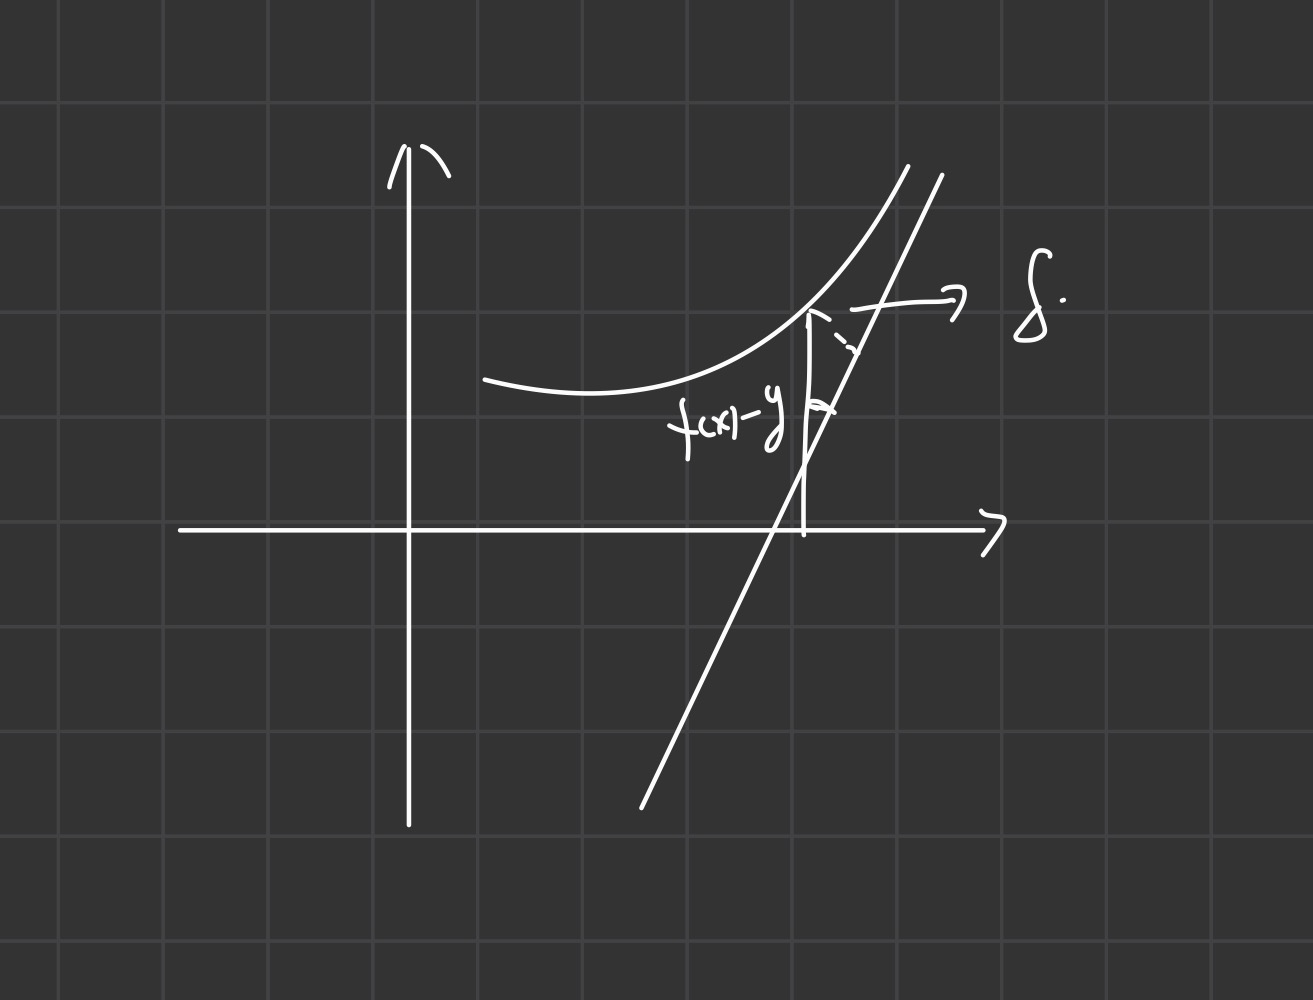
\includegraphics[width=5cm, height=4cm]{images/asymptotic_line.jpg}
\end{center}
它们之间的距离$\delta$和纵坐标的差$|y-Y|$的比值是一个常数,即$Y=ax+b$和$x$轴夹角的余弦值,因此在$x \to +\infty$,这差也随着$\delta$而趋于零,即
$$
\lim\limits_{x \to \infty} (y-ax-b) = 0,
$$
这式子就立马给定了
$$
\lim\limits_{x \to \infty} (y-ax) =b;
$$
再除以$x$,就得
$$
\lim\limits_{x \to \infty} \frac{y}{x} = a;
$$
反过来这两个极限就确定$Y=ax+b$的系数. 
\end{proof}

\subsection{弧长定义}

\begin{definition}
\rm 光滑曲线$\widehat{AB}$上的可能的内接折线周长$p$构成的集合的上确界$S$,叫做$\widehat{AB}$的长,即
$$
S = \sup\{p\}.
$$
如果这个数$S$有限,则曲线叫做\redt{可求长}.
\end{definition}

\begin{proposition}
\rm \redt{曲线参数方程表示} 若曲线$\widehat{AB}$可以用参数方程
$$
x = \varphi(t), \, y = \psi(t) 
$$
表示. 其中$\varphi(t),\psi(t)$都有连续导数. 在$\widehat{AB}$上一点$M$,则$\widehat{AM}$的弧长可以用参变量为$t$的可微分函数$s = s(t)$表示,它的导数为
$$
s'(t) = \lim\limits_{\Delta t \to 0}\frac{\Delta s}{\Delta t} = \sqrt{[\varphi'(t)]^2+[\psi'(t)]^2}.
$$
或者,简单地
$$
s_t' = \sqrt{x_t'^2 + y_t'^2}. 
$$
\end{proposition}

\begin{proposition}
\rm \redt{曲线的函数表示} 若曲线$\widehat{AB}$可以用方程$y=y(x)$表示,$f(t)$有连续导数. 在$\widehat{AB}$上一点$M$,则$\widehat{AM}$的弧长可以用参变量为$x$的可微分函数$s = s(x)$表示,它的导数为
$$
s'(x) = \sqrt{1+y'^2(x)}. 
$$
或者,简单地
$$
s_x' = \sqrt{1+y'^2}.
$$
\end{proposition}

\begin{proposition}
\rm \redt{曲线的极坐标表示} 若曲线$\widehat{AB}$可以用极坐标方程
$$
\rho = \rho(\theta)
$$
表示,那么对应的参数方程为
$$
\left \{
\begin{array}{ll}
x = \rho\cos\theta \\
y = \rho\sin\theta
\end{array} \right.
$$
在$\widehat{AB}$上一点$M$,则$\widehat{AM}$的弧长可以用参变量为$\theta$的可微分函数$s = s(\theta)$表示,它的导数为
$$
s_\theta' = \sqrt{(p'\cos\theta-p\sin\theta)^2 +(p'\sin\theta+p\cos\theta)^2} = \sqrt{\rho^2(\theta) + \rho'^2(\theta)}.
$$
或者,简单地
$$
s_\theta' = \sqrt{\rho^2 + \rho'^2}. 
$$
\end{proposition}

\subsection{弧长微分}

\begin{proposition}
\rm 若曲线$\widehat{AB}$可以用参数方程
$$
x = \varphi(t), \, y = \psi(t) 
$$
表示. 那么弧长微分为
$$
ds = \sqrt{x_t'^2 + y_t'^2}dt
$$
\end{proposition}

\begin{proposition}
\rm  若曲线$\widehat{AB}$可以用方程$y=y(x)$表示. 那么弧长微分为
$$
ds = \sqrt{1+y'^2} dx. 
$$
\end{proposition}

\begin{proposition}
\rm 若曲线$\widehat{AB}$可以用极坐标方程
$$
\rho = \rho(\theta)
$$
表示. 那么弧长微分为
$$
ds = \sqrt{\rho^2+\rho'^2}d\theta
$$
\end{proposition}

\subsection{质心和形心}

\begin{proposition}
\rm 设平面曲线$L$, 其密度函数为$f(x,y)$,则曲线的质心$(\overline{x},\overline{y})$为
$$
\overline{x} = \frac{\int_L xf(x,y)ds}{\int_L f(x,y)ds}, \overline{y} = \frac{\int_L yf(x,y)ds}{\int_L f(x,y)ds}.
$$
类似地,可以推广到空间曲线
$$
\overline{x} = \frac{\int_L xf(x,y,z)ds}{\int_L f(x,y,z)ds}, \overline{y} = \frac{\int_L yf(x,y,z)ds}{\int_L f(x,y,z)ds},
\overline{y} = \frac{\int_L zf(x,y,z)ds}{\int_L f(x,y,z)ds}.
$$
若密度函数是一个常数,即密度是均匀的,则$L$的形心为
$$
\overline{x} = \frac{\int_L xds}{\int_L f(x,y,z)ds}, \overline{y} = \frac{\int_L yds}{\int_L f(x,y,z)ds},
\overline{y} = \frac{\int_L zds}{\int_L f(x,y,z)ds}.
$$
\end{proposition}

\begin{proposition}
\rm 设封闭区域$D$,其密度函数为$f(x,y)$,则区域的质心为$(\overline{x},\overline{y})$为
$$
\overline{x} = \frac{\int\int_D xf(x,y)d\sigma}{\int\int_D f(x,y)d\sigma}, \overline{y} = \frac{\int\int_D yf(x,y)d\sigma}{\int\int_D f(x,y)d\sigma}.
$$
类似地,可以推广到空间区域$V$,则$V$的质心为
$$
\overline{x} = \frac{\int\int\int_V xf(x,y,z)d\sigma}{\int\int_D f(x,y)d\sigma}, 
\overline{y} = \frac{\int\int\int_V yf(x,y,z)d\sigma}{\int\int_D f(x,y)d\sigma},
\overline{z} = \frac{\int\int\int_V zf(x,y,z)d\sigma}{\int\int_D f(x,y,z)d\sigma}.
$$
\end{proposition}

\subsection{曲率}

\subsection{坐标轴下的体积}

\begin{definition}
\rm 圆锥体积的公式
$$
V = \frac{1}{3}sh,
$$
其中$s$是圆锥底面面积,$h$是圆锥的高. 
\end{definition}

\newpage
\section{曲线积分}

\subsection{第一类曲线积分}
\begin{definition}
\rm 设函数$f(x,y)$定义在光滑的可求长的平面曲线$L$上,将$L$分为有限段弧
$\sigma_1,\sigma_2,\cdots,\sigma_n$. 用$\sigma_i$表示第$i$段弧,也表示其弧长. 在每一$\sigma_i$上任取一点$(\xi_i,\eta_i)$,做积分和
$$
\sigma = \sum\limits_{i = 1}^n f(\xi_i,\eta_i)\sigma_i.
$$
用$\lambda$表示$\sigma_1,\sigma_2,\cdots,\sigma_n$中最长的弧长. 当$\lambda \to 0$时,积分和$\sigma$有一确定的有限极限$I$,即与曲线$L$的细分方法无法,由于弧$\sigma$上点$(\xi_i,\eta_i)$的选择无关,则称这一极限为函数$f(x,y)$沿曲线或者道路$L$上所取的\redt{第一类曲线积分}
(对弧长的积分),记为
$$
I = \int_L f(x,y)ds. 
$$
其中$s$表示曲线的弧长,$ds$象征弧元长度$\sigma_i$.
\end{definition}

\begin{proposition}
\rm 第一类曲线积分与路径的方法无关
$$
\int_{L_{AB}} f(x,y)ds = \int_{L_{BA}} f(x,y)ds
$$
\end{proposition}


\begin{proposition}
\rm \redt{化为普通一元定积分} 若平面曲线$L$用$\widehat{AB}$表示,且$\widehat{AB}$上任意一点$M$的位置也由$\widehat{AM}$的弧长来唯一确定,那么$L$可由参数方程
$$
x = \varphi(s), \, y = \psi(s) ~ (0 \leq s \leq S).
$$
则
$$
\int_L f(x,y)ds = \int_{0}^S f(\varphi(s),\psi(s))ds.
$$
\end{proposition}

\begin{proposition}
\rm \redt{参数方程下弧长可微分} 若平面曲线$L$可由参数方程
$$
x = \varphi(t), \, y = \psi(t) (\alpha \leq t \leq \beta)
$$
表示,其中$\varphi(t),\psi(t)$都有连续导数. 且弧长$s = \widehat{AM} = s(t)$的增加对应于参数$t$的增加,则
$$
s_t' = \sqrt{[\varphi'(t)]^2+[\psi'(t)]^2}.
$$
那么有
$$
\int_L f(x,y)ds = \int_\alpha^\beta f(\varphi(t),\psi(t))\sqrt{[\varphi'(t)]^2+[\psi'(t)]^2}dt. 
$$
\end{proposition}

\begin{proposition}
\rm \redt{特殊的参数方程} 若曲线$L$由连续可导函数
$$
y=y(x) ~ (a \leq x \leq b)
$$
给出,其中$y(x)$有连续导数. 那么
$$
\int_L f(x,y)ds = \int_a^b f(x,y(x))\sqrt{1+ [y'(x)]^2}dx. 
$$
\end{proposition}

\begin{proposition}
\rm \redt{极坐标下对弧长积分} 若曲线$L$由连续可导函数
$$
\rho = \rho(\theta) ~ (\alpha \leq \theta \leq \beta).
$$
则
$$
\int_L f(x,y)ds = \int_\alpha^\beta f(\rho\cos\theta,\rho\sin\theta)\sqrt{\rho^2+\rho'^2}d\theta
$$
\end{proposition}

\subsection{第二类曲线积分}

\begin{definition}
\rm 将第一类曲线积分的积分变量换成部分弧长$\sigma_1$的在$x$轴或者$y$上的投影$\Delta x_i$或者$\Delta y_i$,于是得到了\redt{第二类曲线积分}
$$
I_x = \int_L f(x,y)dx,\, I_y = \int_L f(x,y)dy.
$$
若沿曲线$L$定义两个函数$P(x,y)$和$Q(x,y)$,且积分
$$
\int_L P(x,y)dx , \int_L Q(x,y)dy 
$$
都存在,则它们的和就称为\redt{一般形状的曲线积分},记为
$$
\int_L P(x,y)dx + Q(x,y)dy.
$$
\end{definition}

\begin{proposition}
\rm 第二类曲线积分和曲线方向有关
$$
\int_{L_{AB}} f(x,y)dx = -\int_{L_{BA}} f(x,y)dx
$$
同样,
$$
\int_{L_{AB}} f(x,y)dy = -\int_{L_{BA}} f(x,y)dy
$$
\end{proposition}

\begin{proposition}
\rm \redt{给定参数方程下的第二类曲线积分的计算} 若平面曲线$L=\widehat{AB}$可由参数方程
$$
x = \varphi(t), \, y = \psi(t) (\alpha \leq t \leq \beta)
$$
表示,其中$\varphi(t),\psi(t)$都是连续的,且导数$\varphi't(t)$存在且连续,又当参数$t$自$\alpha$变到$\beta$时所确定的点在曲线$L$上以$A$到$B$的方向移动. 则有等式
$$
\int_{L_{AB}}f(x,y)dx = \int_\alpha^\beta f(\varphi(t),\psi(t))\varphi'(t)dt. 
$$
成立. 若导数$\psi't(t)$也存在且连续,给定两个连续函数$P(x,y)$及$Q(x,y)$,则有
$$
\int_{L_{AB}} Pdx + Qdy = \int_\alpha^\beta [P(\varphi(t),\psi(t))\varphi'(t) + Q(\varphi(t),\psi(t))\psi'(t)]dt.
$$
\end{proposition}

\subsection{两种不同类型曲线积分之间的联系}

\begin{proposition}
\rm 给定一光滑曲线$L=\widehat{AB}$,取$L$上任意一点$M$,以其弧长为参数$s=\widehat{AM}$,则可以用参数方程
$$
x=x(s),y=y(s) ~ (0 \leq s \leq S)
$$
表示$L$. 若以$\alpha$表示弧的增加方向的切线与$x$轴间的夹角. 即有
$$
\cos \alpha = x'(s), \, \sin \alpha = y'(s).
$$
因此我们有
$$
\int_{L_{AB}} f(x,y)dx = \int_0^S f(x(s),y(s))x'(s)ds = \int_{L_{AB}} f(x,y)\cos \alpha ds.
$$
同理考虑第二类曲线积分的一般形式则有
$$
\int_{L_{AB}}Pdx+Qdy = \int_{L_{AB}} (P\cos\alpha +Q\sin\alpha)ds.
$$
\end{proposition}

\newpage
\subsection{曲线积分与道路无关的条件}

\begin{annotation}
\rm 曲线积分$\int_L Pdx + Qdy$与\redt{道路无关}是指这个积分只与曲线$L$的起点和终点有关,与其两点的路径形状无关. 
\end{annotation}

\begin{theorem}\label{line-integral: path-independent}
\rm 设在一个单连通域$D$上有两个连续函数$P(x,y),Q(x,y)$. 给定$D$上任意一个光滑曲线,曲线积分$\int_L Pdx + Qdy$结果与\redt{道路无关}的充分必要条件是: $Pdx+Qdy$是某一个二元函数的全微分. 
\end{theorem}

\begin{proof}
\rm \emph{必要性}\ 若曲线积分$\int_L Pdx + Qdy$在$D$上与道路无关,给定两点$D$上两点$A(x_0,y_0),B(x_1,y_1)$,那么此时我们可以用记号
$$
\int_{(x_0,x_0)}^{(x_1,y_1)} Pdx+Qdy
$$
来表示原曲线积分. 现在我们固定点$A$,用$M$表示$D$中任意一点$(x,y)$,我们来考虑辅助函数
$$
F(x,y) = \int_{(x_0,y_0)}^{(x,y)} Pdx+Qdy.
$$
那么当$M=B$时,我们有
$$
F(x_1,x_2) = \int_{(x_0,x_0)}^{(x_1,y_1)} Pdx+Qdy.
$$
现在在点$B$的基础上给$x_1$一增量$\Delta x$是它变成点$C(x_1+\Delta x,y_1)$,在$\Delta x$充分小的时候,直线段$BC$也在$D$中. 于是对应函数增量为
$$
F(x_1+\Delta x ,y_1)-F(x_1,y_1) = \int_{\overline{BC}}Pdx+ Qdy = \int_{\overline{BC}} Pdx,
$$ 
其中因为$BC$垂直于$y$轴的,所以$Qdy$的积分为零. 因为$P(x,y)$连续,所以我们可以用一下中值定理有
$$
F(x_1+\Delta x ,y_1)-F(x_1,y_1) = \Delta x P(x_1+\theta \Delta x,y_1),  0 \leq \theta \leq 1.
$$
于是我们有
$$
\frac{F(x_1+\Delta x ,y_1)-F(x_1,y_1)}{\Delta x} = P(x_1+\theta \Delta x, y_1).
$$
还是由于$P(x,y)$的连续性,当$\Delta x \to 0$时,上述等式的右边趋于$P(x_1,y_1)$,而左边是$F(x,y)$关于$x$的偏导数定义. 因此我们有
$$
\frac{\partial F(x_1,y_1)}{\partial x} = P(x_1,y_1). 
$$
同理我们可得
$$
\frac{\partial F(x_1,y_1)}{\partial y} = Q(x_1,y_1). 
$$
故$F(x,y)$有两个连续偏导,因此最终
$$
dF = \frac{\partial F(x_1,y_1)}{\partial x}dx + \frac{\partial F(x_1,y_1)}{\partial y}dy = Pdx +Qdy.
$$
\emph{充分性}\ 若$P=\frac{\partial \Phi}{\partial x},\,Q=\frac{\partial \Phi}{\partial y}$. 给定两点$D$上两点$A(x_0,y_0),B(x_1,y_1)$,设任意一条光滑的曲线$\widehat{AB}$对应的参数方程表示为
$$
x = \varphi(t),\, y = \psi(t).
$$
对应$A,B$两点的参数表示为
$$
x_0 = \varphi(\alpha),y_0 =\psi(\alpha);\; x_1 =\varphi(\beta), y_1 = \psi(\beta).
$$
我们还需要假定当$t$从$\alpha$变动到$\beta$时,对应的点在曲线上从$A$变动到$B$. 现在沿曲线$\widehat{AB}$来计算积分,则有
$$
\int_{\widehat{AB}}Pdx+ Qdy = \int_\alpha^\beta \{P(\varphi(t),\psi(t))\varphi'(t) + Q(\varphi(t),\psi(t))\psi'(t)\}dt
$$
那么实际上根据复合多元函数的规则,设$u = \Phi(\varphi(t),\psi(t)) $有
$$
du = \frac{\partial u}{\partial x}\varphi'(t)dt + \frac{\partial u}{\partial y}\psi'(t)dt.
$$
因此我们有
$$
\int_\alpha^\beta \{P(\varphi(t),\psi(t))\varphi'(t) + Q(\varphi(t),\psi(t))\psi'(t)\}dt = \int_\alpha^\beta \frac{d}{dt} \Phi(\varphi(t),\psi(t)).
$$
最后
$$
\int_{\widehat{AB}}Pdx+ Qdy = \Phi(x_1,y_1)-\Phi(x_0,y_0). 
$$
\end{proof}

\begin{proposition}
\rm \redt{\ref{line-integral: path-independent} 判别方法} 设在一个单连通域$D$上有两个连续函数$P(x,y),Q(x,y)$,且它们具有\redt{一阶连续偏导}. 则$Pdx + Qdy$是一个二元函数的全微分的充分必要条件为
$$
\frac{\partial P}{\partial y} = \frac{\partial Q}{\partial x}
$$
在$D$上恒成立. 
\end{proposition}

\begin{proof}
\rm \emph{必要性}\ 若$P = \frac{\partial \Phi}{\partial x},
\,Q = \frac{\partial \Phi}{\partial y}$. 于是
$$
\frac{\partial P}{\partial y} = \frac{\partial^2\Phi}{\partial x\partial y},\,\frac{\partial Q}{\partial x} = \frac{\partial^2\Phi}{\partial y\partial x}.
$$
因为$P$及$Q$都有一阶连续偏导,由\ref{mixed-derivatives: exchange-order},所以有$\frac{\partial P}{\partial y} = \frac{\partial Q}{\partial x}$.

\emph{充分性}\ 若$\frac{\partial P}{\partial y} = \frac{\partial Q}{\partial x}$,我们来求原函数,它要满足
$$
\frac{\partial \Phi}{\partial x} = P,
\, \frac{\partial \Phi}{\partial y} = Q.
$$
因为$P$及$Q$是连续的,我们来对它们分别积分. 我们在$D$中选取两点$x,x_0$,固定一个$y$. 再对$P(x,y)$做关于$x$从$x_0$到$x$的积分,即有
$$
\Phi(x,y) - \Phi(x_0,y) = \int_{x_0}^{x} P(t,y)dt. 
$$
再选取$y_0$,对$Q(x_0,y)$做关于$y$从$y_0$到$y$的积分,就有
$$
\Phi(x_0,y)-\Phi(x_0,y_0) = \int_{y_0}^{y} Q(x_0,t)dt. 
$$
综上于是有
$$
\Phi(x,y) = \int_{x_0}^{x} P(t,y)dt + \int_{y_0}^{y} Q(x_0,t)dt + \Phi(x_0,y_0).
$$
其中$\Phi(x_0,y_0)$为确定的任意常数. 我们需要来验证一下$\Phi(x,y)$是否符合我们的要求,分别来对它取偏导数. 对$x$取偏导时,等式后面两项与$x$无关的,所以很容易得到$\frac{\partial \Phi}{\partial x} = P(x,y)$; 对$y$取偏导时,第二项可以容易得到$Q(x_0,y)$,第一项需要应用一下\redt{莱布尼茨法则}(fz509),有
$$
\int_{x_0}^{x}P(t,y)dt = \int_{x_0}^{x} \frac{\partial P(t,y)}{\partial y}dt.
$$ 
根据条件可以将$\frac{\partial P(t,y)}{\partial y}$替换成$\frac{\partial Q(t,y)}{\partial x}$,于是最终上面这个积分的结果就是
$Q(x,y)-Q(x_0,y)$,所以也有$\frac{\partial \Phi}{\partial y} = Q(x,y)$.

\end{proof}

\begin{proposition}
\rm \redt{道路无关下第二类曲线积分的计算} 若曲线积分$\int_L P(x,y)dx + Q(x,y)dy$与道路无关,则有
$$
\int_{(x_1,x_2)}^{(y_1,y_2)} Pdx + Qdy = \int_{x_1}^{x_2} P(x,y_1)dx + \int_{y_1}^{y_2} Q(x_2,y)dx. 
$$ 
及
$$
\int_{(x_1,x_2)}^{(y_1,y_2)} Pdx + Qdy = \int_{y_1}^{y_2} P(x_1,y)dy + \int_{x_1}^{2_2} Q(x,y_2)dx. 
$$
\bluet{变成了两个平行于坐标轴的直线的积分}.
\end{proposition}

\subsection{闭路积分}

\begin{lemma}
\rm 若积分$\int_L Pdx+Qdy$取在沿不论怎样的简单(即不自身相交)闭路上永远等于零,则它即使区在任何自身相交的闭路上也将为零.
\end{lemma}

\begin{theorem}
\rm 曲线积分$\int_{\widehat{AB}} Pdx+Qdy$与道路无关当且仅当闭路积分$\int_L Pdx+Qdy$沿任何闭路都等于零. 
\end{theorem}

\newpage
\section{二重积分}

\subsection{二重积分的定义}
\begin{definition}
\rm 设函数$z=f(x,y)$定义在有界闭区域$\mathcal{D}$上,将区域$\mathcal{D}$任意分成$n$个小闭区域
$$
\Delta\sigma_1,\Delta\sigma_2,\cdots,\Delta\sigma_n.
$$
用$\Delta\sigma_i$表示第$i$小区域,也表示它的面积. 在每个$\Delta\sigma_i$上任取一点$(\xi_i,\eta_i)$,将在这一点处的函数值$f(\xi_1,\eta_i)$乘上对应区域的面积$\Delta\sigma_i$,并将所有类似的乘积相加所得的和
$$
\sigma = \sum\limits_{i=1}^n f(\xi_i,\eta_i)\Delta\sigma_i
$$
称为函数$f(x,y)$在区域$\mathcal{D}$上的\redt{积分和}. 以$\lambda$表示$n$个小区域中的最大直径. 若当$\lambda \to 0$时积分和$\sigma$有一确定的有限极限
$$
I = \lim\limits_{\lambda \to 0}\sigma,
$$
既与区域$\mathcal{D}$分为$n$小区域的分法无关,又与在每一个小区域上点$(\xi_i,\eta_i)$选法也无关. 则称这一极限为函数$f(x,y)$在区域$\mathcal{D}$上的\redt{二重积分}并记做
$$
I = \int\int_{\mathcal{D}}f(x,y)d\mathcal{\sigma}
$$
\end{definition}

\begin{annotation}
\rm 一点集中任意两点距离的上确界称为该点集的直径. 
\end{annotation}

\begin{proposition}
\rm 可积函数必须是有界的.
\end{proposition}

\begin{annotation}
\rm \redt{几何意义} 当$f(x,y) \geq 0$时,二重积分$\int\int_D f(x,y)d\sigma$等于以区域$D$为底,曲面$z=f(x,y)$的为曲顶的曲顶柱体的体积. 
\end{annotation}

\subsection{二重积分的性质}

\begin{annotation}
\rm 常规性质与一重积分相符.
\end{annotation}

\begin{proposition}
\rm 设可积函数$f(x,y)$定义在有界闭区域$\mathcal{D}$上,若沿着一在$\mathcal{D}$中的光滑曲线改变$f(x,y)$的函数值. 则只要不破坏$f(x,y)$有界性,且改变后的$f(x,y)$依然可积,且它的积分等于$f(x,y)$的积分
\end{proposition}

\begin{annotation}
\rm 类别一重定积分中改变有限多个点的函数值不改变整体的积分值.
\end{annotation}

\begin{theorem}
\rm \redt{推广的中值定理} 若可积函数$f(x,y)$在区域$\mathcal{D}$上满足
$$
m \leq f(x,y) \leq M.
$$
则
$$
m\sigma \leq \int\int_{\mathcal{D}}f(x,y)d\sigma \leq M\sigma.
$$
特别地,若$f(x,y)$在$\mathcal{D}$上连续,则$\mathcal{D}$上存在一点$(\xi,\eta)$使得
$$
\int\int_{\mathcal{D}}f(x,y)d\sigma = f(\xi,\eta)\sigma.
$$
\end{theorem}

\subsection{二重积分的计算}

\begin{theorem}
\rm \redt{在矩形区域的情况下化为二重积分为逐次积分} 如对定义于矩形$\mathcal{D}[a,b;c,d]$上的一函数$f(x,y)$二重积分存在,且对每一个$[a,b]$上的常数值$x$,单积分
$$
I(x) = \int_c^d f(x,y)dy (a \leq x \leq b)
$$
也存在,则逐次积分
$$
\int_a^b dx \int_c^d f(x,y)dy
$$
同样存在,且等式
$$
\int\int_{\mathcal{D}}f(x,y)d\sigma = \int_a^b dx \int_c^d f(x,y)dy
$$
也成立. 若单积分
$$
I'(x)\int_a^b f(x,y)dx.
$$
也存在,那么
$$
\int_a^b dx \int_c^d f(x,y)dy = \int_c^d dy \int_a^b f(x,y)dx
$$
\end{theorem}

\begin{annotation}
\rm 特别地$f(x,y)$是连续的,则一定有上面的定理成立.
\end{annotation}

\begin{theorem}
\rm \redt{在曲边区域的情况下化二重积分为逐次积分} 如果$f(x,y)$定义于由上下两条曲边$\varphi_2(x),\varphi_1(x)$围成的区域$\mathcal{D}$时,且$f(x,y)$在$\mathcal{D}$上的二重积分存在,又对$[a,b]$中每一个固定值$x$单积分
$$
I(x) = \int_{\varphi_1(x)}^{\varphi_2(x)} f(x,y)dy
$$ 
也存在. 则逐次积分
$$
\int_a^b dx \int_{\varphi_1(x)}^{\varphi_2(x)} f(x,y)dy
$$
也同样存在,且等式
$$
\int\int_{\mathcal{D}}f(x,y)d\sigma = \int_a^b dx \int_{\varphi_1(x)}^{\varphi_2(x)} f(x,y)dy
$$
也存在. 
\end{theorem}

\begin{annotation}
\rm \bluet{这里有一个需要注意的地方,曲边$\varphi_2(x),\varphi_1(x)$和平行于纵坐标直线需要只有两个交点. 这个很重要!不然你就需要考虑换积分次序了}.
\end{annotation}

\begin{proposition}
\rm \redt{变量代换} 设$f(x,y)$是定义在区域$D$上的连续函数,变换
$$
\left \{
\begin{array}{ll}
x = x(u,v)\\
y = y(u,v)
\end{array}
\right.
$$
定义在$D'$上,把$D'$一一映射到$D$上,且$x(u,v),y(u,v)$有一阶连续偏导,其雅克比行列式
$$
\frac{D(x,y)}{D(u,v)} \neq 0.
$$
则有
$$
\int\int_D f(x,y)dxdy = \int\int_D' f(x(u,v),y(u,v))\left| \frac{D(x,y)}{D(u,v)} \right| dudv
$$
\end{proposition}

\begin{proposition}
\rm \redt{在极坐标下计算二重积分} 设区域$D$的参数方程为
$$
\left \{
\begin{array}{ll}
x = \rho \cos \theta \\
y = \rho \sin \theta 
\end{array} \right.
$$
其中$(\rho,\theta)$满足$D = \Set{(\rho,\theta)}{\varphi_1(\theta) \leq \rho \leq \varphi_2(\theta), \alpha \leq \theta \leq \beta}$. 则
$$
\int\int_D f(x,y)d\sigma = \int_\alpha^\beta d\theta \int_{\varphi_1(\theta)}^{\varphi_2(\theta)} f(\rho\cos \theta,\rho\sin\theta)\rho d\rho.
$$
其中
$$
\left|\frac{D(x,y)}{D(\rho,\theta)}\right| = \begin{vmatrix}
\cos\theta &-\rho\sin\theta \\
\sin\theta & \rho\cos\theta 
\end{vmatrix} = \rho.
$$
\end{proposition}

\begin{annotation}
\rm 适合用极坐标计算的二重积分的特征
\begin{enumerate}
	\item 被积函数: $f(\sqrt{x^2+y^2}),f(\frac{y}{x}),f(\frac{x}{y})$.
	\item 积分域: $x^2+y^2 \leq R, r^2 \leq x^2+y^2 \leq R, x^2+y^2 \leq 2ax, x^2+y^2 \leq 2bx$. 
\end{enumerate}
\end{annotation}

\subsection{格林公式}

\begin{definition}
\rm \redt{闭路方向} 在平面的右手定向的情况下,我们规定一闭路的方向如下: 当观察者沿闭路的一方向行走时,若闭路围成的区域考虑观察者的左手,我们就称这一方向是\redt{正的}; 反之就是负的. 
\end{definition}

\begin{theorem}
\rm \redt{格林公式} 设闭区域$D$由分段光滑的曲线$L$围成,若函数$P(x,y)$及$Q(x,y)$在$D$上具有一阶连续偏导数,则有
$$
\int\int_D \left( \frac{\partial Q}{\partial x} - \frac{\partial P}{\partial x} \right) = \int_L Pdx+Qdy.
$$
其中$L$是$D$的取正向的边界曲线. \bluet{它可以将二重积分转换成对闭路曲线的积分,同样反过来可以把对闭路曲线的积分转换称对区域的二重积分}. 
\end{theorem}

\begin{annotation}
\rm 当下我们可以配合格林公式来证明沿闭路曲线积分为零的充要条件
$$
\frac{\partial P}{\partial y} = \frac{\partial Q}{\partial x}.
$$
充分性是显然的,函数值为$0$的积分结果肯定还是$0$. 证必要性可以假设在区域$D$上某一点$M$使得
$$
\frac{\partial P}{\partial y} \neq \frac{\partial Q}{\partial x}.
$$
不妨设$\frac{\partial P}{\partial y} - \frac{\partial Q}{\partial x} > \eta$,由于$\frac{\partial P}{\partial y} ,\frac{\partial Q}{\partial x}$都是连续的,所以可以找到一个$M$的充分小的邻域使得$\frac{\partial P}{\partial y} - \frac{\partial Q}{\partial x} > \frac{\eta}{2}$,显然在这个邻域里面取一条闭路曲线沿着它积分的结果肯定是不可能为零的. 
\end{annotation}

\newpage
\section{曲面积分}

\subsection{双侧曲面}

\begin{definition}
\rm 在光滑曲面$S$上任取一点 ,过点$M_0$的法线有两个方向,如果选定法线的某个方向为指定的方向,当点在曲面上连续移动时,法线也连续变动、当动点从$M_0$出发沿着曲面上任意一条不越过曲面边界的封闭曲线又回到原位置$M_0$时,法线的指向保持不变,称这种曲面为\redt{双侧曲面},否则称其为\redt{单侧曲面}.
\end{definition}

\begin{annotation}
\rm 什么叫法线方向的确定详细理解看菲砖.
\end{annotation}

\subsection{曲面面积}

\begin{definition}
\rm 设给定一个闭光滑曲面$S$. 将曲面$S$分成$n$个部分曲面
$$
S_1, S_2,\cdots,S_n,
$$
$S_i$同时也代表第$i$个部分曲面的面积. 并在每个部分曲面$S_i$内任意地选取一点$M_i(i=1,2,\cdots,n)$,把$S_i$垂直地投影到曲面在点$M_i$处的切面上,得到在投影面积记为$T_i$. 这些面积$T_i$的和在个部分曲面$S_i$的直径趋于$0$时的极限$L$称为曲面$S$的面积. 若用$\lambda$表示所有部分曲面$S_i$中的直径最大值,即有
$$
\lim\limits_{\lambda \to 0}\sum\limits_{i=1}^n T_i = L.
$$
\end{definition}

\begin{proposition}
\rm 设曲面$S$由方程
$$
z=f(x,y)
$$
给出,其中$(x,y)$在$xOy$平面上的区域$D$内变动,函数$f(x,y)$在$D$上有一阶连续偏导. 则曲面$S$的面积为
$$
A = \int\int_D\sqrt{1+f_x^2(x,y),f_y^2(x,y)}dxdy.
$$
有
$$
dA = \frac{d\sigma}{\cos \gamma}.
$$
其中$\cos\gamma$表示$f(x,y)$法向量和$z$轴的夹角余弦值. 
\end{proposition}

\subsection{第一类曲面积分}

\begin{annotation}
\rm 对面积的积分.
\end{annotation}

\begin{definition}
\rm 设曲面$S$是光滑且闭的,函数$f(x,y,z)$在$S$上有界. 把$S$任意分成$n$个部分曲面$S_i(i=1,2,\cdots,n)$,$S_i$同时也表示第$i$块部分曲面的面积. 设$M_i(\xi_i,\eta_i,\zeta_i)$是$S_i$上任意取定的一点,做乘积$f(\xi_i,\eta_i,\zeta_i)S_i(i=1,2,\cdots,n)$,并做和$\sum\limits_{i=1}^n f(\xi_i,\eta_i,\zeta_i)S_i$,如果当各部分曲面的直径的最大值$\lambda \to 0$时,这和的极限总存在,且不依赖曲面$S$的分法和点$M_i$的选择,则这极限叫做函数$f(x,y,z)$沿曲面$S$的第一类曲面积分,记为
$$
I = \int\int_{S} f(x,y,z)dS = \lim\limits_{\lambda \to 0}\sum\limits_{i=1}^n f(\xi_i,\eta_i,\zeta_i)S_i.
$$
\end{definition}

\begin{proposition}
\rm \redt{化为二重积分的计算方法} 设曲面$S$由方程$z=f(x,y)$给出,其中$(x,y)$在$xOy$平面的区域$D$变动,函数$f(x,y)$在$D$上有连续偏导. 则有
$$
\int\int_S f(x,y,z)dS = \int\int_D f(x,y,f(x,y))\sqrt{1+f_x^2(x,y)+f_y^2(x,y)}dxdy. 
$$
其中$dS = \sqrt{1+f_x^2(x,y)+f_y^2(x,y)}dxdy$
\end{proposition}

\subsection{第二类曲面积分}

\begin{annotation}
\rm 对有向面积的积分.
\end{annotation}

\begin{definition}
\rm \redt{第二类曲面积分}定义与第一类曲面积分定义形式上相似,即
$$
I = \int\int_{S} f(x,y,z)d\sigma_{xy} =\int\int_{S} f(x,y,z)dxdy= \lim\limits_{\lambda \to 0}\sum\limits_{i=1}^n f(\xi_i,\eta_i,\zeta_i)\sigma_{xy_i}.
$$
其中$\sigma_i$表示$S_i$在平面$xOy$的投影,那么即有
$$
S_i = \frac{\sigma_i}{\cos \gamma},
$$
其中$\gamma$表示当且确定方向的法向量与$z$轴的夹角,所以其余弦值是有正有负的. 类似地,在其他两个平面$xOz$及$yOz$上也有
$$
I = \int\int_{S} f(x,y,z)d\sigma_{xz} =\int\int_{S} f(x,y,z)dxdz= \lim\limits_{\lambda \to 0}\sum\limits_{i=1}^n f(\xi_i,\eta_i,\zeta_i)\sigma_{xz_i}.
$$
及
$$
I = \int\int_{S} f(x,y,z)d\sigma_{yz} =\int\int_{S} f(x,y,z)dydz= \lim\limits_{\lambda \to 0}\sum\limits_{i=1}^n f(\xi_i,\eta_i,\zeta_i)\sigma_{yz_i}.
$$
那么一般形式为
$$
\int\int_{S} P(x,y,z)dydz + Q(x,y,z)dzdx + R(x,y,z)dxdy.  
$$
\end{definition}

\begin{proposition}
\rm  \redt{第二类曲面积分化二重积分} 若曲面由方程$z=f(x,y)$确定,其$(x,y)$在平面$xOy$上的区域$D_{xy}$变动,函数$f(x,y)$在$D$上有连续偏导. 取$S$为上侧,则每点法向量与$z$轴的夹角余弦值为正,则有
$$
\int\int_{S} f(x,y,z)dxdy = \int\int_{D_{xy}} f(x,y,f(x,y))dxdy.
$$
\end{proposition}

\newpage
\section{三重积分}

\subsection{三重积分定义}
\begin{definition}
\rm 设函数$f(x,y,z)$定义在有界闭的区域$\mathcal{V}$上,将$\mathcal{V}$分成有限个部分区域
$$
v_1,v_2,\cdots,v_n.
$$
用$\Delta v_i$表示第$i$个部分区域,也表示它的体积. 在每个$\Delta v_i$上任取一点$(\xi_i,\eta_i,\zeta_i)$,将这一点处的函数值$f(\xi_i,\eta_i,\zeta_i)$乘上对应区域的体积$v_i$,并做积分和
$$
\sigma = \sum\limits_{i = 1}^nf(\xi_i,\eta_i,\zeta_i)v_i.
$$
以$d$表示$n$个部分区域的最大直径. 若当$d \to 0$时积分和$\sigma$有一确定的有限极限$I$,则称$I$是$f(x,y,z)$在$\mathcal{V}$上的三重积分,记为
$$
I = \int\int\int_{\mathcal{V}} f(x,y,z)d\sigma.
$$
\end{definition}

\subsection{三重积分的性质}

\begin{definition}
\rm 常规性质和二重积分相符.
\end{definition}

\begin{proposition}
\rm 三重积分的存在及大小与函数在光滑曲面上的取值无关. 
\end{proposition}

\begin{proposition}
\rm \redt{中值定理的推广}
\end{proposition}

\subsection{三重积分的计算}

\begin{theorem}
\rm \redt{平行六面体的三重积分计算} 若对函数$f(x,y,z)$在$\mathcal{V}[a,b;c,d;e,f]$上的三重积分存在,且若对$[a,b]$中每一固定的$x$,二重积分
$$
I(x) = \int\int_{R}f(x,y,z)d\sigma_1
$$
存在,则逐次积分
$$
\int_a^b dx \int\int_{R}f(x,y,z)d\sigma_1
$$
也存在,且等式
$$
\int\int\int_{\mathcal{V}} f(x,y,z)d\sigma = \int_a^b dx \int\int_{R_{yz}}f(x,y,z)d\sigma_1.
$$
同样若单重极限
$$
\int_e^f f(x,y,z)dz
$$
存在,则
$$
\int\int\int_{\mathcal{V}} f(x,y,z)d\sigma = \int\int_{R_{xy}}\int_e^f f(x,y,z)dz.
$$
\end{theorem}

\begin{proposition}
\rm \redt{柱坐标下的三重积分} 将直角坐标转化为柱坐标,即
$$
\left\{
\begin{array}{ll}
x = \rho\cos\theta \\
y = \rho\sin\theta \\
z = z
\end{array}\right.
$$
其中$\rho$表示圆柱底圆半径长度,$\theta$表示半径与$x$轴的夹角,则对应的三重积分为
$$
\int\int\int_{\Omega}f(x,y,z)dv = \int\int\int_{\Omega} f(\rho\cos\theta,\rho\sin\theta,z)\rho d\rho d\theta dz.  
$$
\end{proposition}

\begin{proposition}
\rm \redt{球坐标下的三重积分} 将直角坐标转化为球坐标,即
$$
\left\{
\begin{array}{ll}
x = r\rho\sin\varphi\cos\theta \\
y = r\rho\sin\varphi\sin\theta \\
z = r\cos\varphi
\end{array}\right.
$$
其中$r$表示半径长度,$\varphi$为半径与$z$轴的夹角,$\theta$为半径在$x0y$上的投影和$x$轴的夹角,则三重积分为
$$
\int\int\int_{\Omega}f(x,y,z)dv = \int\int\int_{\Omega} f(r\rho\sin\varphi\cos\theta,r\rho\sin\varphi\sin\theta,r\cos\varphi)
r^2\sin\varphi dr d\varphi d\theta.
$$
其中
$$
\frac{D(x,y,z)}{D(r,\varphi,\theta)} =  \begin{pmatrix}\sin \varphi \cos \theta &r\cos \varphi \cos \theta &-r\sin \varphi \sin \theta \\ \:\:\sin \varphi \sin \theta &r\cos \varphi \sin \theta &r\sin \varphi \cos \theta \\ \:\:\cos \varphi &-r\sin \varphi &0\end{pmatrix} = r^2\sin\varphi.
$$
\end{proposition}

\subsection{斯托克斯公式}

\begin{theorem}
\rm 设$L$为空间分段光滑的有向闭曲线,$\sum$是以$L$为边界的分片光滑曲面$L$,$L$的方向与$\sum$的法方向符合右手法则,函数$P,Q,R$在$\sum$上具有一阶连续偏导数,则有
$$
\begin{array}{ll}
\int_L P(x,y,z)dx + Q(x,y,z)dy + R(x,y,z)dz &= 
\int\int_\sum
\begin{vmatrix}
\cos \alpha & \cos \beta & \cos \gamma \\
\frac{\partial}{\partial x} & \frac{\partial}{\partial y} & \frac{\partial}{\partial x} \\
P & Q & R
\end{vmatrix} dS \\
&= \int\int_\sum (\frac{\partial R}{\partial y}-\frac{\partial Q}{\partial z})dydz + (\frac{\partial P}{\partial z}-\frac{\partial R}{\partial x})dzdx + (\frac{\partial Q}{\partial x}-\frac{\partial P}{\partial y})dxdy
\end{array}
$$
\end{theorem}

\newpage
\section{常数项无穷级数}

\subsection{无穷级数的基本概念}

\begin{definition}
\rm 设给定某一无穷序列
\begin{equation}
a_1,a_2,\cdots,a_n,\cdots.
\end{equation}
由这些数所做的符号
\begin{equation}
a_1 + a_2 + \cdots + a_n + \cdots
\end{equation}
叫做\redt{(常数项)无穷级数},而$(1)$中各数叫做级数的项. 利用累加符号可将(2)记为
$$
\sum\limits_{n=1}^\infty a_n.
$$
(1)的前$n$项和
$$
s_n = a_1+a_2+\cdots+a_n
$$
称为(1)的\redt{部分和}.
\end{definition}

\begin{definition}
\rm 若级数$\sum\limits_{n=1}^\infty a_n$的部分和构成的数列$(s_n)$有有限极限$s$,即
$$
\lim\limits_{n \to \infty} s_n = S,
$$
那么就称无穷级数$\sum\limits_{n=1}^\infty a_n$\redt{收敛},这时$S$叫做这级数的和,即
$$
\sum\limits_{n=1}^\infty a_n = \lim\limits_{n \to \infty} s_n = S.
$$
反之若$(s_n)$没有有限极限,无穷级数$\sum\limits_{n=1}^\infty a_n$\redt{发散}.
\end{definition}

\begin{example}
\rm \redt{几何级数的收敛性} 讨论$\sum\limits_{n=0}^{+\infty}aq^n$的收敛性.

由几何级数的求和公式有
$$
s_n  =  \left \{
\begin{array}{ll}
\frac{a(q^{n}-1)}{q-1} & q\neq 1\\
na & q = 1
\end{array} \right.
$$

当$|q| < 1$,则有$\lim\limits_{n \to \infty} \frac{a(q^{n}-1)}{q-1} = \frac{a}{q-1}$,则级数收敛.

当$|q| > 1$,则有$\lim\limits_{n \to \infty} \frac{a(q^{n}-1)}{q-1} = \infty$,则级数发散.

当$q = 1$,显然级数是发散的; 当$q = -1$时,$n$为偶数时,$s_n =0$,$n$为奇数时,$s_n=a$,则级数发散. 

综上,当$|q| < 1$时,几何级数收敛; 当$|q| \geq 1$时,几何级数发散.   
\end{example}

\begin{example}
\rm \redt{调和级数的收敛性} 讨论$\sum\limits_{n=1}^{\infty} \frac{1}{n^p}$的收敛性.

当$p \leq 1$时,熟知最通常的调和级数$s_n = \sum\limits_{n=1}^{\infty} \frac{1}{n}$是发散的,当$p <1$时级数中的各项是大于$p=1$的级数各项,所以$p < 1$时也是发散的. 综上$p \leq 1$时,调和级数发散. 

当$p > 1$时,这里借助一个不等式
$$
\frac{1}{(n+1)^p} + \frac{1}{(n+2)^p} + \cdots + \frac{1}{(2n)^p} < n \cdot \frac{1}{n^p}.  
$$
记$\sigma = p-1$,因此分组
$$
\underbrace{1+\frac{1}{2^p}},\underbrace{\frac{1}{3^p}+\frac{1}{4^p}}_{\frac{1}{2^\sigma}},\underbrace{\frac{1}{5^p}+\frac{1}{6^p}+\frac{1}{7^p}+\frac{1}{8^p}}_{\frac{1}{4^\sigma}},\cdots
$$
于是
$$
s_n <  1 + \frac{1}{2^p} + \frac{\frac{1}{2^\sigma}}{1-\frac{1}{2^\sigma}}. 
$$
所以当$p > 1$时调和级数收敛. 
\end{example}
\subsection{收敛级数的基本性质}

\begin{definition}
\rm 如果舍弃级数$\sum\limits_{n=1}^\infty a_n$前面的$m$个项,得到级数
$$
a_{m+1} + a_{m+2} + \cdots + a_{m+k} + \cdots = \sum\limits_{n=m+1}^\infty a_n,
$$
称其为级数$\sum\limits_{n=1}^\infty a_n$的第$m$项后的\redt{余式}. 
\end{definition}

\begin{proposition}\label{series-convergence: remnant-convergence}
\rm \redt{余式收敛性} 如果级数$\sum\limits_{n=1}^\infty a_n$收敛,则它的任何一个余式$\sum\limits_{n=m+1}^\infty a_n$也收敛; 反之,从余式的收敛性可推出原来级数$\sum\limits_{n=1}^\infty a_n$的收敛性. \bluet{换句话说,丢弃级数前面的有限个项或者在级数前面加进若干新的项,并不影响级数的收敛性}.
\end{proposition}

\begin{proof}
\rm 固定$m$,用$s_k'$表示余式$\sum\limits_{n=m+1}^\infty a_n$的部分和. 于是
\begin{equation}
s_k' = s_{m+k} - s_m.
\end{equation}
若级数$\sum\limits_{n=1}^\infty a_n$收敛,那么有
$$
\lim\limits_{k \to \infty}s_k' = S-s_m = S',
$$
即级数$\sum\limits_{n=m+1}^\infty a_n$也收敛. 

反之若级数$\sum\limits_{n=m+1}^\infty a_n$收敛于$S'$,将(1)式的$k=n-m$得到
$$
s_n = s_m + s_{n-m}'.
$$
再取两边取极限,则有
$$
\lim\limits_{n \to \infty} s_n  = s_m + S',
$$
即级数$\sum\limits_{n=1}^\infty a_n$也是收敛的. 
\end{proof}

\begin{proposition}
\rm \redt{收敛则余式趋于零} 设级数$\sum\limits_{n=1}^\infty a_n$第$m$项后的余式的和为$r_n$,若级数$\sum\limits_{n=1}^\infty a_n$收敛,则$r_n$随着$m$的增大而趋于$0$.
\end{proposition}

\begin{proof}
若$\sum\limits_{n=1}^\infty a_n$收敛于$S$,于是
$$
r_m = S - s_m,
$$
因此$m$增大的时候$s_m$也在增大且趋于$S$,所以$r_m$随之减少至$0$.
\end{proof}

\begin{proposition}
\rm 如果级数$\sum\limits_{n=1}^\infty a_n$收敛$S$,那么级数$\sum\limits_{n=1}^\infty ca_n$也收敛,且其和为$cS$. 
\end{proposition}


\begin{proposition}
\rm \redt{可加性} 若两个级数$\sum\limits_{n=1}^\infty a_n$及$\sum\limits_{n=1}^\infty b_n$分布收敛于$S_a$和$S_b$,那么级数$\sum\limits_{n=1}^\infty (a_n \pm b_n)$也收敛,且其和为$S_a \pm S_b$.
\end{proposition}

\begin{proposition}
\rm \redt{可结合性} 若级数$\sum\limits_{n=1}^\infty a_n$收敛,那么对这级数的项任意加括号之后所成的级数仍收敛,其和不变.
\end{proposition}

\begin{proposition}
\rm \redt{级数收敛的必要条件} 若级数$\sum\limits_{n=1}^\infty a_n$收敛,那么其通项$a_n$趋于$0$. 
\end{proposition}

\begin{proof}
显然有
$$
a_n = s_n - s_{n-1}.
$$
\end{proof}

\subsection{正项级数的收敛性}

\begin{definition}
\rm 若级数的每一项都是非负的,称其为\redt{正项级数}. 
\end{definition}

\begin{theorem}
\rm \redt{正项级数收敛的基本定理} 如果正向级数的部分和上有界,则其收敛; 反之则发散. \bluet{类似于数列极限中的单调有界数列必有极限}.
\end{theorem}


\begin{theorem}
\rm \redt{最基础的比较审敛法}  若给定两个正向级数$\sum\limits_{n=1}^\infty a_n$和$\sum\limits_{n=1}^\infty b_n$. 若从某项其$n > N$,恒有$a_n \leq b_n$成立,那么若级数$\sum\limits_{n=1}^\infty b_n$收敛,则$\sum\limits_{n=1}^\infty a_n$也收敛; 若级数$\sum\limits_{n=1}^\infty a_n$发散,则$\sum\limits_{n=1}^\infty b_n$也发散.
\end{theorem}


\begin{theorem}\label{positive-series: compare-convergence}
\rm 如果极限
$$
\frac{a_n}{b_n} = K
$$
存在,则级数$\sum\limits_{n=1}^\infty a_n$和$\sum\limits_{n=1}^\infty b_n$同时收敛或者同时发散.
\end{theorem}

\begin{theorem}
\rm 如果从某项起$n > N$,恒有
$$
\frac{a_{n+1}}{a_n} \leq \frac{b_{n+1}}{b_n}
$$
成立,那么若级数$\sum\limits_{n=1}^\infty b_n$收敛,则$\sum\limits_{n=1}^\infty a_n$也收敛; 若级数$\sum\limits_{n=1}^\infty a_n$发散,则$\sum\limits_{n=1}^\infty b_n$发散. 
\end{theorem}

\begin{proof}
在不失一般性的情况下,可以认为命题给出的条件在所有$n=1,2,3,\cdots$都是成立的,即
$$
\frac{a_2}{a_1} \leq \frac{b_2}{b_1},\frac{a_3}{a_2} \leq \frac{b_3}{b_2}, \cdots, \frac{a_{n}}{a_{n-1}} \leq \frac{b_{n}}{b_{n-1}}.
$$
逐项将这些不等式相乘,我们可以得到
$$
\frac{a_{n}}{a_1} \leq \frac{b_{n}}{b_1},
$$
移项即得
$$
a_n \leq \frac{a_1}{b_1}\cdot b_n. 
$$
而级数$\sum\limits_{n=1}^\infty \frac{a_1}{b_1}\cdot b_n$和$\sum\limits_{n=1}^\infty b_n$收敛性相同,类似\ref{positive-series: compare-convergence}.
\end{proof}

\begin{proposition}
\rm \redt{柯西判别法} 若当$n$充分大的时候有
$$
\sqrt[n]{a_n} \leq q \Leftrightarrow a_n \leq q^n
$$
成立,其中$0 < q <1$,则级数$\sum\limits_{n=1}^\infty a_n$收敛; 如果从某处开始有
$$
\sqrt[n]{a_n} \geq 1,
$$
则级数发散. 前提条件可以用数列极限语言表示为
$$
\lim\limits_{n \to \infty} \sqrt[n]{a_n} = q,
$$
当$0 < q <1$时级数收敛,而当$q >1$时级数发散. \bluet{当$q=1$时无法判定}. 
\end{proposition}

\begin{proposition}
\rm \redt{达朗贝尔判别法} 若当$n$充分大的时候有
$$
\frac{a_{n+1}}{a_n} \leq q
$$
成立,其中$0 < q <1$,则级数$\sum\limits_{n=1}^\infty a_n$收敛; 如果从某处开始有
$$
\frac{a_{n+1}}{a_n} \geq 1,
$$
则级数发散. 前提条件可以用极限语言表示为
$$
\lim\limits_{n \to \infty} \frac{a_{n+1}}{a_n} = q.
$$
\end{proposition}

\begin{annotation}
\rm \bluet{柯西判别法和达朗贝尔都是以几何级数为标准而导出的比较审敛法}.
\end{annotation}

\begin{theorem}
\rm \redt{拉阿伯判别法} 若当$n$充分大的时候有
$$
n\left( \frac{a_n}{a_{n+1}} - 1\right) \geq r
$$
成立,其中$r > 1$,则级数$\sum\limits_{n=1}^\infty a_n$收敛; 若从某项起
$$
n\left( \frac{a_n}{a_{n+1}} - 1\right) \leq 1
$$
则级数发散. 
\end{theorem}

\begin{proof}
设在$n$充分大的时候,有
$$
\frac{a_n}{a_{n+1}} \geq  1 + \frac{r}{n}.
$$
取$1< s < r$,我们有
$$
\lim\limits_{n \to \infty} \frac{(1+\frac{1}{n})^s-1}{\frac{1}{n}} = s.
$$
于是在$n$充分大的时候,有
$$
(1+\frac{1}{n})^s \leq 1+\frac{r}{n}. 
$$
因此
$$
\frac{a_n}{a_{n+1}} \geq (1+\frac{1}{n})^s,
$$
故
$$
\frac{a_{n+1}}{a_n} \leq \frac{\frac{1}{(1+n)^s}}{\frac{1}{(n)^s}}.
$$
\end{proof}

\begin{annotation}
\rm \bluet{拉阿伯判断法是以调和级数为标准而导出的比较审敛法}.
\end{annotation}

\begin{proposition}
\rm \redt{积分判别法} 若
$$
\sum\limits_{n=1}^\infty a_n \equiv \sum\limits_{n=1}^\infty f(n).
$$
其中$f(x)$是连续的,正的单调递减函数. 级数$\sum\limits_{n=1}^\infty a_n$的收敛,取决于函数
$$
F(x) = \int f(x)dx
$$
当$x \to +\infty$时是否有有限极限. 
\end{proposition}

\begin{proof}
其中$F(x)$是$f(x)$的一个原函数,由于$f(x) > 0$,所以$F(x)$也是一个单调增函数,我们考虑这样一个级数
\begin{equation}
\sum\limits_{n=1}^{\infty} \left[F(n+1)-F(n)\right].
\end{equation}
由中值定理,有
$$
F(n+1)-F(n) = f(n+\theta),\, 0 < \theta < 1.
$$
于是
$$
a_{n+1} = f(n+1) < F(n+1)-F(n) < f(n)=a_n. 
$$
因此若级数(1)收敛,那么$\sum\limits_{n=1}^{\infty}f(n+1)$也是收敛的,从而$\sum\limits_{n=1}^{\infty}f(n)$也是收敛的. 
\end{proof}


\newpage
\subsection{任意项级数的收敛性}

\begin{theorem}
\rm \redt{数列柯西收敛原理的推广} 级数$\sum\limits_{n=1}^{\infty}a_n$收敛的充要条件为: 对任意的数$\varepsilon > 0$,存在自然数$n$,使得当$n > N$时,对任意的$m=1,2,3,\cdots$都有
$$
|a_{n+1}+a_{n+2}+\cdots+a_{n+m}| \leq \varepsilon.
$$
特别地,当$m=1$时,就得到了级数收敛的必要条件. 
\end{theorem}

\begin{theorem}
\rm \redt{绝对收敛} 设给定级数$\sum\limits_{n=1}^{\infty}a_n$. 若由这个级数的项的绝对值所组成的级数$\sum\limits_{n=1}^{\infty}|a_n|$收敛,则给定级数也收敛.
\end{theorem}

\begin{theorem}
\rm 若级数$\sum\limits_{n=1}^{\infty}a_n$和它的绝对值级数$\sum\limits_{n=1}^{\infty}|a_n|$同时收敛,则称级数$\sum\limits_{n=1}^{\infty}a_n$\redt{绝对收敛}. 若级数$\sum\limits_{n=1}^{\infty}a_n$收敛,而其绝对值级数$\sum\limits_{n=1}^{\infty}|a_n|$不收敛,则称级数$\sum\limits_{n=1}^{\infty}a_n$\redt{非绝对收敛}(条件收敛).
\end{theorem}

\begin{annotation}
\rm 注意绝对值级数发散,但是其原级数是可能收敛的. \bluet{但是使用柯西判别法和达朗贝尔办法在这里依然有效,即在这种情况判别绝对值级数发散,那么原级数一定也是发散的}. 
\end{annotation}

\begin{proposition}
\rm \redt{绝对收敛级数的可交换性} 若级数$\sum\limits_{n=1}^{\infty}a_n$绝对收敛,则把它的项重新排列后得到的级数$\sum\limits_{k=1}^{\infty}a_k'$也收敛并且具有与原级数相同的和. 
\end{proposition}

\begin{proof}
先证正项级数重排不影响原级数的和,说明重排之后绝对收敛的性质不变. 再证在绝对收敛的情况下,级数的和可以表示成级数中正项的和减去负项绝对值的和,说明原级数的和不变.  
\end{proof}

\begin{theorem}
\rm \redt{黎曼定理} 若级数$\sum\limits_{n=1}^{\infty}a_n$条件收敛,则无论预选取怎样的数$A$,都可以重排这级数中的项,使得得到的新级数的和为$A$. \bluet{Amazing}!
\end{theorem}

\begin{annotation}
\rm \bluet{条件收敛这是由于正项和负项的相互抵消才能实现}. 
\end{annotation}

\subsection{幂级数}

\begin{definition}
\rm 形如
$$
\sum\limits_{n=0}^{\infty}a_nx^n =  a_0 + a_1x+ a_2x^2 + \cdots + a_nx^n + \cdots
$$
的级数,被称为\redt{幂级数}.
\end{definition}

\begin{theorem}
\rm 若对于异于$0$的值$x=\bar{x}$使得级数$\sum\limits_{n=0}^{\infty}a_nx^n$收敛,则对于任意的$|x| < |\bar{x}|$的,都可以使得级数$\sum\limits_{n=0}^{\infty}a_nx^n$绝对收敛.
\end{theorem}

\begin{proof}
若级数$\sum\limits_{n=0}^{\infty}a_n\bar{x}^n$收敛,那么其通项有界,即
$$
|a_n\bar{x}^n| \leq M, n = 0,1,2,\cdots.
$$
现在任取$x$使得$|x| < |\bar{x}|$,考虑级数$\sum\limits_{n=0}^{\infty}|a_nx^n|$的收敛性. 我们有
$$
|a_nx^n| = |a_n\bar{x}^n|\cdot \left|\frac{x}{\bar{x}}\right|^n \leq M\cdot\left|\frac{x}{\bar{x}}\right|^n,
$$
显然级数$\sum\limits_{n=0}^{\infty} M\cdot\left|\frac{x}{\bar{x}}\right|^n$是一个收敛的几何级数,因此$\sum\limits_{n=0}^{\infty}|a_nx^n|$收敛. 
\end{proof}


\begin{definition}
\rm 若存在一些使得级数$\sum\limits_{n=0}^{\infty}a_nx^n$收敛而异于$0$的$x = \bar{x}$,若所有这样的点构成的集合$\{\bar{x}\}$上有界,而$R$是它的上确界,则称$R$是级数$\sum\limits_{n=0}^{\infty}a_nx^n$的\redt{收敛半径}. 当$|x| < R$时,级数$\sum\limits_{n=0}^{\infty}a_nx^n$决定收敛; 当$|x| > R$时,级数$\sum\limits_{n=0}^{\infty}a_nx^n$发散. 
\end{definition}

\begin{theorem}
\rm \redt{用系数表示收敛半径} 给定幂级数$\sum\limits_{n=0}^{\infty}a_nx^n$. 若
$$
\lim\limits_{n \to \infty} \left|\frac{a_{n+1}}{a_n}\right| = \rho,
$$
那么这幂级数的收敛半径为
$$
R = \left\{ \begin{array}{ll}
\frac{1}{\rho}, & \rho \neq 0 \\
+\infty, & \rho = 0 \\
0, & \rho = +\infty
\end{array}\right.
$$
\end{theorem}

\begin{proof}
\rm 当$\rho=0$时,对任意$x \neq 0$,都有
$$
\lim\limits_{n \to \infty}\frac{|a_{n+1}x^{n+1}|}{|a_{n}x^n|} = \left|\frac{a_{n+1}}{a_n}\right|\cdot |x| = 0.
$$
由达朗贝尔判别可以知$\sum\limits_{n=0}^{\infty}a_nx^n$收敛. 因此$R = +\infty$ 

当$\rho = +\infty$时,同理对任意$x \neq 0$,都有
$$
\lim\limits_{n \to \infty}\frac{|a_{n+1}x^{n+1}|}{|a_{n}x^n|} = \left|\frac{a_{n+1}}{a_n}\right|\cdot |x| = \infty.
$$
可知$\sum\limits_{n=0}^{\infty}a_nx^n$发散. 因此$R = 0$.

当$0 < \rho < +\infty$时,对任意$x \neq 0$,都有
$$
\lim\limits_{n \to \infty}\frac{|a_{n+1}x^{n+1}|}{|a_{n}x^n|} = \left|\frac{a_{n+1}}{a_n}\right|\cdot|x|  = \rho x.
$$
因此我们让$\rho x < 1$即可,即$x < \frac{1}{\rho}$. 
\end{proof}

\begin{theorem}
\rm \redt{幂级数的有理运算} 设幂级数$\sum\limits_{n=0}^{\infty}a_nx^n$的收敛半径为$R_1$,$\sum\limits_{n=0}^{\infty}a_nx^n$的收敛半径为$R_2$,则$\sum\limits_{n=0}^{\infty}a_nx^n$和$\sum\limits_{n=0}^{\infty}a_nx^n$都在$|x| < min(R_1,R_2)$上收敛. 对应的有理运算
$$
\begin{array}{ll}
\sum\limits_{n=0}^{\infty}a_nx^n \pm \sum\limits_{n=0}^{\infty}a_nx^n = \sum\limits_{n=0}^{\infty}(a_n,b_n)x^n \\ 
\left(\sum\limits_{n=0}^{\infty}a_nx^n \right) \cdot \left( \sum\limits_{n=0}^{\infty}b_nx^n \right) = a_0b_0  + (a_0b_1+a_1b_0)x + \cdots + (a_0b_n + \cdots a_nb_0)x^n +\cdots \\
\frac{\sum\limits_{n=0}^{\infty}a_nx^n}{\sum\limits_{n=0}^{\infty}b_nx^n} = \sum\limits_{n=0}^{\infty}c_nx^n, \sum\limits_{n=0}^{\infty}a_nx^n  =  \sum\limits_{n=0}^{\infty}b_nx^n \cdot \sum\limits_{n=0}^{\infty}c_nx^n
\end{array}
$$
也在$|x| < min(R_1,R_2)$上收敛. 
\end{theorem}

\begin{proposition}
\rm 设幂级数$\sum\limits_{n=0}^{\infty}a_nx^n$的收敛半径为$R$,函数$S(x) = \sum\limits_{n=0}^{\infty}a_nx^n$. 则函数$S(x)$在$(-R,R)$上连续.
\end{proposition}

\begin{proposition}
\rm 设幂级数$\sum\limits_{n=0}^{\infty}a_nx^n$的收敛半径为$R$,函数$S(x) = \sum\limits_{n=0}^{\infty}a_nx^n$. 则函数$S(x)$在$(-R,R)$上可导,且可逐项可导,即
$$
S'(x) = \sum\limits_{n=1}^{\infty}na_nx^{n-1},
$$
其对应的幂级数与原幂级数有相同的收敛半径. \bluet{但其收敛域可能变大}.
\end{proposition}

\begin{proposition}
\rm 设幂级数$\sum\limits_{n=0}^{\infty}a_nx^n$的收敛半径为$R$,函数$S(x) = \sum\limits_{n=0}^{\infty}a_nx^n$. 则函数$S(x)$在$(-R,R)$上可积,且可逐项可积,即
$$
\int_0^x S(t)dt  = \sum\limits_{n=0}^{\infty} \frac{a_n}{n+1}x^{n+1}.
$$
其对应的幂级数与原幂级数有相同的收敛半径. \bluet{但其收敛域可能变大}.
\end{proposition}

\begin{example}
\rm \redt{利用分析求和函数} 求幂级数$\sum\limits_{n=1}^{\infty} \frac{x^n}{n(n+1)}$的和函数. 

由于
$$
\lim\limits_{n \to \infty} \frac{\frac{1}{(n+1)(n+2)}}{\frac{1}{n(n+1)}} = 1,
$$
所以$S(x)$的收敛半径为$1$. 这里有
$$
(xS(x))' = \sum\limits_{n=1}^{\infty} \frac{x^n}{n}.
$$
再求导一次有
$$
(xS(x))'' = \sum\limits_{n=1}^{\infty} x^{n-1} = \frac{1}{1-x}. 
$$
再反过来积分
$$
(xS(x))'  = \int_0^{x} \frac{1}{1-x}dx = -\ln (1-x) + C,
$$
由前面可知$(xS(x))'|_{x=0} = 0$,这里$C  = 0$. 再积分
$$
xS(x)  = \int_0^{x} -\ln(1-x)dx = (1-x)\ln(1-x)+x.
$$
那么即有
$$
S(x) = \left\{\begin{array}{ll}
\frac{(1-x)\ln (1-x)}{x} + 1, x \in (-1,1), x \neq 0 \\
0, x = 0
\end{array} \right.
$$
注意明显原级数在$\pm = 1$是收敛的,终有
$$
S(x) = \left\{\begin{array}{ll}
\frac{(1-x)\ln (1-x)}{x} + 1, x \in [-1,1), x \neq 0 \\
0, x = 0 \\
1, x = 1 
\end{array} \right.
$$
\end{example}

\subsection{交错级数}

\begin{definition}
\rm 形如
$$
c_1 - c_2 + c_3 - c_4 + \cdots + (-1)^{n-1}c_n + \cdots,
$$
其中$c_n > 0,n=1,2,\cdots$,这样的级数称为\redt{交错级数}.
\end{definition}

\begin{theorem}
\rm \redt{莱布尼茨定理} 若交错级数的项的绝对值单调递减,即
$$
c_{n+1} \leq c_n
$$
并趋于$0$,则级数收敛.
\end{theorem}

\begin{proof}
考察偶数项个的部分和$C_{2m}$,即
$$
C_{2m} = (c_1-c_2) + (c_3 - c_4) + \cdots + (c_{2m-1}-c_{2m}).
$$
其中每一项都是正的,所以$C_{2m}$是随着$m$的增大而增大. 另一方面上述的部分和还可以写成
$$
C_{2m} = c_1 - (c2-c_3) - (c_4-c_5) - \cdots - (c_{2m-2}-c_{2m-1}) - c_{2m},
$$
因此$C_{2m} \leq c_1$,即$C_{2m}$上有界的. 结合前述结论,可知当$m \to \infty$时$C_{2m}$有有限极限. 而奇数项的部分和可以写成
$$
C_{2m-1} = C_{2m} + c_{2m}, 
$$
等式两边取极限,可得$\lim\limits_{m \to \infty} C_{2m-1}=C_{2m}$.   因此所有部分都有有限极限. 
\end{proof}

\subsection{两个数列依次相乘组成的级数}


\begin{theorem}
\rm \redt{阿贝尔判定法} 若级数$\sum\limits_{n=1}^{+\infty}a_n$收敛,而数列$b_n$单调有界,则级数$\sum\limits_{n=1}^{+\infty}a_nb_n$收敛. 
\end{theorem}

\begin{theorem}
\rm \redt{狄利克雷判定法} 若级数$\sum\limits_{n=1}^{+\infty} a_n$部分和总是有界,而数列$b_n$单调有界,则级数$\sum\limits_{n=1}^{+\infty} a_nb_n$收敛. 
\end{theorem}

\newpage
\subsection{初等函数的展开}

\begin{theorem}
\rm 设函数$f(x)$在点$x_0$的某一邻域$U(x_0)$内具有任意阶的导数,则$f(x)$在该邻域内能展开成泰勒级数的充分必要条件是在该邻域内$f(x)$的泰勒公式中的余项$R_n(x)$当$n \to \infty$时的极限为零,即
$$
\lim\limits_{n \to \infty} R_n(x) = 0, x \in U(x_0).
$$
\end{theorem}

\begin{proof}
由\ref{series-convergence: remnant-convergence}可知. 
\end{proof}

\begin{theorem}
\rm \redt{泰勒级数展开的判定} 设函数$f(x)$在点$x_0$的某一邻域$[0,H]$内具有任意阶的导数,并且在给定区间上变化时,所有这些导数的绝对值有上界,即
$$
|f^{(n)}(x)| \leq L,
$$
其中$L$不依赖$n$,则$f(x)$在该邻域上能被展开成泰勒级数. 
\end{theorem}

\begin{proof}
假定在$x=0$处展开,取拉格朗日余项$R_n(x)$,我们有
$$
|R_n(x)| = \frac{|f^{(n+1)}(\theta x)|}{(n+1)!}|x|^{n+1} \leq L \cdot \frac{|H|^{n+1}}{(n+1)!}.
$$
当$n \to \infty$时,$\frac{|H|^{n+1}}{(n+1)!}$是趋于零的,从收敛级数$\sum\limits_{n=0}^{\infty} \frac{|H|^{n+1}}{(n+1)!}$的必要性是可知的. 
\end{proof}


\begin{proposition}
\rm 下述函数在$x=0$处的泰勒展开对任意$x$都收敛:
\begin{enumerate}
	\item $e^x = 1 + \frac{x}{1!} + \frac{x^2}{2!} + \cdots + \frac{x^n}{n!} + \cdots$;
	\item $\sin x = {x} - \frac{x^3}{3!} + \frac{x^5}{5!} - \cdots + (-1)^{k-1}\frac{x^{2k-1}}{(2k-1)!} + \cdots,k =1,2,\cdots$;
	\item $\cos x = 1 - \frac{x^2}{2!} +  \frac{x^4}{4!} - \cdots + (-1)^{k-1}\frac{2^{2k-2}}{(2k-2)!} + \cdots , k=1,2,\cdots$;
	\item $\text{sh} x = x + \frac{x^3}{3!} + \frac{x^5}{5!}+ \cdots + \frac{x^{2k-1}}{(2k-1)!}, k = 1,2,\cdots$;
	\item $\text{ch} x = 1 + \frac{x^2}{2!} + \frac{x^4}{4!}+ \cdots + \frac{x^{2k}}{(2k)!}, k =0,1,\cdots$;
\end{enumerate}
\end{proposition}

\begin{proposition}
\rm 下述函数在$x=0$处的泰勒展开在$(-1,1)$上收敛
\begin{enumerate}
	\item $\frac{1}{1-x} = 1+x+x^2+\cdots+x^n + \cdots$;
	\item $\frac{1}{1+x} = 1-x+x^2+\cdots+(-1)^nx^n + \cdots$.
	\item $(1+x)^\alpha = 1 + \alpha x+ \frac{\alpha(\alpha-1)}{2!}x^2 +  \cdots + \frac{\alpha(\alpha-1)\cdots(\alpha-n+1)}{n!}x^n+\cdots$,两个端点处是否收敛取决于$\alpha$的取值. 
\end{enumerate}
\end{proposition}

\begin{proposition}
\rm 
$$
\arctan x = x - \frac{x^3}{3} + \frac{x^5}{5} - \cdots + (-1)^{k-1}\frac{x^{2k-1}}{2k-1} + \cdots,k=1,2,\cdots.
$$
仅在区间$[-1,1]$上收敛. 
\end{proposition}

\begin{proposition}
\rm 
$$
\ln (1+x) = x-\frac{x^2}{2} + \frac{x^3}{3}- \cdots + (-1)^{k-1}\frac{x^k}{k},k=1,2,\cdots,
$$
仅在区间$(-1,1]$上收敛. 
\end{proposition}

\begin{annotation}
\rm \redt{间接展开法} 根据泰勒展开的唯一性,从某些已知函数的展开式出发,利用幂级数的性质(四则运算,逐项求导,逐项积分)以及变量代换等方法,求得所给函数的展开式.
\end{annotation}

\begin{example}
\rm 求$\arctan x$的$x$的泰勒展开级数.

\rm 由于
$$
\frac{1}{1+x} = \sum\limits_{n=1}^{\infty} (-1)^{n-1}x^{n-1}, x \in (-1,1), 
$$
于是
$$
\frac{1}{1+x^2} = \sum\limits_{n=1}^{\infty} (-1)^{n-1}x^{2n-2}, x \in (-1,1). 
$$
对上式两边积分,则有
$$
\arctan x = \sum\limits_{n=1}^{\infty} \int_0^{x} (-1)^{n-1}x^{2n-2}  =   \sum\limits_{n=1}^{\infty}(-1)^{n-1}\frac{x^{2n-1}}{2n-1} = x - \frac{x^3}{3} + \frac{x^5}{3} + \cdots,
$$
显然$\sum\limits_{n=1}^{\infty}(-1)^{n-1}\frac{x^{2n-1}}{2n-1}$在$x = \pm 1$也收敛,即该级数在$x \in [-1,1]$上收敛. 
\end{example}


\newpage
\section{Preliminary}

\subsection{三角函数相关}
\begin{definition}
\rm 弧度定义是{\color{red}描述角度和对应的弧长的一个双射关系},避免在其他运算过程中使用度数的不方便. 弧度定义{\color{red}弧长公式}和{\color{red}扇形面积公式}分别为
$$
l = rx ~\text{和}~ s = \frac{\pi r^2}{2}
$$
\end{definition}

\begin{proposition}
\rm 三角函数
$$
\begin{array}{ll}
\sin x & \text{正弦} \\
\cos x & \text{余弦} \\
\tan x & \text{正切} \\
\sec x = \frac{1}{\cos x} & \text{正割} \\
\csc x = \frac{1}{\sin x} & \text{余割} \\
\cot x = \frac{1}{\tan x} & \text{余切} \\
\end{array}
$$
c~co~余~补角
\end{proposition}

\begin{proposition}
\rm 基本关系式
\begin{enumerate}
	\item $\tan x = \frac{\sin x}{\cos x}$;
	\item $\sin^2 x + \cos^2 x =1$;
	\item $1 + \tan^2 x = \sec^2 x$;
\end{enumerate}
\end{proposition}

\begin{proposition}
\rm 三角函数周期性的相关性质
$$
\begin{array}{ll}
\sin (x+\frac{\pi}{2}) &= \cos x \\
\sin (x+\pi) &= -\sin x \\
\sin (x+\frac{3\pi}{2}) &= -\cos x \\
\sin (x+2\pi) &= \sin x \\
\cos (x+\frac{\pi}{2}) &= -\sin x \\
\cos (x+\pi) &= -\cos x \\
\cos (x+\frac{3\pi}{2}) &= \sin x \\
\cos (x+2\pi) &= \cos x \\
\end{array}
$$
\end{proposition}

\begin{proposition}
\rm 和差角公式
$$
\begin{array}{ll}
\sin(\alpha + \beta) = \sin \alpha \cos \beta + sin \beta \cos \alpha \\
\sin(\alpha - \beta) = \sin \alpha \cos \beta - \sin \beta \cos \alpha \\
\cos(\alpha + \beta) = \cos \alpha \cos \beta - \sin \alpha \sin \beta \\
\cos(\alpha - \beta) = \cos \alpha \cos \beta + \sin \alpha \sin \beta \\
\tan(\alpha + \beta) = \frac{\tan \alpha + \tan \beta}{1-\tan\alpha\tan\beta} \\ 
\tan(\alpha + \beta) = \frac{\tan \alpha + \tan \beta}{1-\tan\alpha\tan\beta} \\
\tan(\alpha - \beta) = \frac{\tan \alpha - \tan \beta}{1+\tan\alpha\tan\beta}
\end{array}
$$
\end{proposition}

\begin{proposition}
\rm 和差化积公式
$$
\begin{array}{ll}
\sin \alpha + \sin \beta = 2\sin\frac{\alpha + \beta}{2}\cos\frac{\alpha - \beta}{2} \\
\sin \alpha - \sin \beta = 2\cos\frac{\alpha + \beta}{2}\sin\frac{\alpha - \beta}{2} \\
\cos \alpha + \cos \beta = 2\cos\frac{\alpha + \beta}{2}\cos\frac{\alpha - \beta}{2} \\
\cos \alpha - \cos \beta = - 2\sin\frac{\alpha + \beta}{2}\sin\frac{\alpha - \beta}{2} \\
\tan \alpha + \tan \beta = \frac{\sin (\alpha + \beta)}{\cos \alpha \sin \beta} 
\end{array}
$$
\end{proposition}

\begin{proposition}
\rm 积化和差公式
$$
\begin{array}{ll}
\cos\alpha \cos\beta = \frac{cos(\alpha+\beta)+cos(\alpha-\beta)}{2} \\
\sin\alpha \sin\beta = \frac{\cos(\alpha-\beta)-\cos(\alpha+\beta)}{2} \\ 
\sin\alpha \cos\beta = \frac{\sin(\alpha+\beta)+\sin(\alpha-\beta)}{2} \\
\cos\alpha \sin\beta = \frac{\sin(\alpha+\beta)-\sin(\alpha-\beta)}{2} \\ 
\end{array}
$$
\end{proposition}

\begin{proposition}
\rm 二倍角公式
$$
\begin{array}{ll}
\sin 2\alpha = 2\sin \alpha \cos \alpha = \frac{2\tan \alpha}{1 + \tan^2 \alpha}\\
\cos 2\alpha = \cos^2 \alpha - \sin^2 \alpha =  2\cos^2\alpha - 1 = 1 - 2\sin^2 \alpha  = \frac{1-\tan^2 \alpha}{1 + \tan^2\alpha}\\
\tan 2\alpha = \frac{2\tan\alpha}{1-\tan^\alpha}
\end{array}
$$
\end{proposition}

\begin{proposition}
\rm 半角公式
$$
\begin{array}{ll}
\sin\frac{\alpha}{2} = \pm \sqrt{\frac{1-\cos \alpha}{2}} \\
\cos\frac{\alpha}{2} = \pm \sqrt{\frac{1+\cos \alpha}{2}} \\
\tan\frac{\alpha}{2} = \sqrt{\frac{1-\cos \alpha}{1+\cos \alpha}} = \frac{1-\cos \alpha}{\sin \alpha} = \frac{\sin \alpha}{1+\cos \alpha}\\
\end{array}
$$
\end{proposition}

\end{document}

